\begin{graphicspathcontext}{{./chapters/ciad/imgs/},{./chapters/appendix/imgs/auto/},\old}

\begin{textpictureframe}{Prof\string.\,Dr\string. St\'ephane GALLAND}{sgalland}
	\vspace{-.25cm}
	\begin{columns}
		\begin{column}{.2\linewidth}
			
\includegraphics[width=\linewidth]{osezlia_couleur}
		\end{column}
		\begin{column}{.8\linewidth}
			\Emph{Ambassador for AI in BFC} \\
			\Emph{Creator \& Director of the CIAD laboratory} \\
			\Emph{Full Professor of Computer Science}
		\end{column}
	\end{columns}
	\vspace{.25cm}
	{\scriptsize Universit\'e de Technologie de Belfort-Montb\'eliard, France} \\[.25cm]
	
	\Emph{Major Topics: Multiagent systems, Multiagent-based simulation, Agent-Oriented Software Engineering} \\[.25cm]

	\scriptsize \begin{tabularx}{\linewidth}{@{}lX@{}}
		Web page: & \url{http://www.ciad-lab.fr/stephane_galland} \\
		Email: & \href{mailto:stephane.galland@utbm.fr}{stephane.galland@utbm.fr} \\
	\end{tabularx} \\[.5cm]

	\scriptsize See also his open-source contributions:\begin{itemize}
		\item Agent Programming Language: \url{http://www.sarl.io}
		\item Agent Modeling: \url{http://www.aspecs.org}
		\item \url{http://www.arakhne.org}
		\item \url{https://github.com/gallandarakhneorg/}
	\end{itemize}

	\putat(87,-103){\includegraphics[width=1.5cm]{sgalland_qrcode}}
\end{textpictureframe}

\end{graphicspathcontext}

\endinput

\begin{graphicspathcontext}{{./talks/utseus/imgs/},{./talks/utseus/imgs/auto/},{./chapters/appendix/imgs/},{./chapters/appendix/imgs/auto/},\old}

\begin{frame}{Evaluation Steps}
	\begin{block}{Lab Work Evaluation}
		At the end of all the tutorial/labwork sessions with \Emph{Prof. Galland}, you will have to send by email (or Wechat) the source code that you had written during the lab work sessions \\
		Date: \Emph{April 24th} \\
		Contribution to the final score: 33\%
	\end{block}
	\begin{block}{Final Exam on Table}
		During the offical week for on-table exams, you will have to pass a final exam on table \\
		Duration: 1 hour 30 minutes \\
		Note: No document or electronic device allowed \\
		Contribution to the final score: 66\%
	\end{block}
\end{frame}

\figureslide{Wexin Group}{wechatqrcode}

\libraryslide[2nd edition]{book_wooldridge}{An Introduction to Multiagent Systems}{Michael~WOOLDRIDGE}{Wiley, May 2009}{0-47-0519460}

\libraryslide[2nd edition]{book_zeigler}{Theory of Modeling and Simulation}{Bernard~ZEIGLER, Herbert~Praehofer, and Tag~Gon~Kim}{Academic Press, 2000}{0-12-7784551}

\end{graphicspathcontext}

\endinput


\part{From Cyber-Physical System to Multiagent Systems}
\begin{bibliographysection}

	\section{Complex Systems}
	\begin{graphicspathcontext}{{./chapters/cps/imgs/},{./chapters/cps/imgs/auto/},\old}

\sidecite{Holland2006ComplexSystems}
\begin{frame}[t]{What is a Complex System?}
	\smaller
	\begin{columns}
		\begin{column}{.5\linewidth}
			\begin{block}{Key characteristics}
				\begin{itemize}
				\item Large number of \emph{interacting components}
				\item \emph{Non-linear} dynamics --- small causes, large effects
				\item \emph{Emergence}: global behaviour not deducible from parts
				\item \emph{Self-organisation} without central control
				\item \emph{Adaptability} to perturbations
				\item Sensitivity to \emph{initial conditions}
				\end{itemize}
			\end{block}
			\smaller
			\begin{exampleblock}{Examples from nature \& society}
				\begin{itemize}
				\item Ant colonies, bird flocks
				\item Brain, immune system
				\item Financial markets, internet traffic
				\item Climate system
				\end{itemize}
			\end{exampleblock}
		\end{column}
		\begin{column}{0.5\linewidth}
			\begin{block}{Formal intuition}
			Let $\Sigma = \{s_1, \dots, s_n\}$ be a set of simple components. \\
			The \emph{emergent} global property $\mathcal{P}$ satisfies:
			\[
			\mathcal{P}(\Sigma) \neq \bigoplus_{i=1}^{n} \mathcal{P}(s_i)
			\]
			The whole is \emph{more than} the sum of its parts
			\end{block}
		\end{column}
	\end{columns}
\end{frame}

\sidecite{Anderson1972MoreIsDifferent}
\begin{frame}{Levels of Description in Complex Systems}
	\begin{columns}
		\begin{column}{.5\linewidth}
			\begin{block}{Micro Level}
				\begin{itemize}
				\item Individual components
				\item Local interactions
				\item Simple rules
				\item Observable states: $s_i \in S$
				\end{itemize}
			\end{block}
			\begin{block}{Macro Level}
				\begin{itemize}
				\item Collective patterns
				\item Global properties
				\item Emergent structures
				\item Phase transitions
				\end{itemize}
			\end{block}
		\end{column}
		\begin{column}{.5\linewidth}
			\begin{alertblock}{The central challenge}
				How do we \Emph{model}, \Emph{predict} and \Emph{engineer} systems
				where macro-level behaviour \Emph{emerges} from micro-level rules?
			\end{alertblock}
			\begin{exampleblock}{Key disciplines}
				\begin{itemize}
				\item Statistical physics
				\item Information theory
				\item \Emph{Artificial Intelligence}
				\item \Emph{Agent-based modelling}
				\end{itemize}
			\end{exampleblock}
		\end{column}
	\end{columns}
\end{frame}

\end{graphicspathcontext}

\endinput


	\section{Artificial Intelligence and Complex Systems}
	\subsection{Definitions of AI}
	\begin{graphicspathcontext}{{./chapters/ai/imgs/},{./chapters/ai/imgs/auto/},\old}

\begin{frame}[c]{What is AI?}
	\begin{definition}[focusing on behavioral mimicry by Minsky 50's]
		AI is the science of programming computers to \emph{perform tasks} that require \emph{intelligence when performed by human beings}
	\end{definition}
	\vspace{1cm}
	\begin{definition}[from OECD-OCDE]
		An AI is a machine-based system that, for \emph{explicit or implicit goals}, deduces from the \emph{inputs} it receives how to generate results such as \emph{forecasts, content, recommendations or decisions} that can influence physical or virtual environments. \emph{Different AI systems} vary in their levels of autonomy and adaptability once deployed
	\end{definition}
\end{frame}

\figureslide{Usages of AI in 2025}{ai_usages_2025}

\sidecite{ElFallahSeghrouchni18}
\begin{frame}[c]{Holistic vision of intelligence (human or artificial)}
	\begin{columns}
		\begin{column}{.5\linewidth}
			\begin{definitionblock}{Intelligence \cite{piaget1947psychologie}}
				Intelligence is what you use when you don't know what to do: when neither innateness nor learning has prepared you for the particular situation
			\end{definitionblock}
		\end{column}
		\begin{column}{.5\linewidth}
			\viconbox*[.49\linewidth]{Cognitive Intelligence}{intelligences-cognitive}
			\hfill
			\viconbox*[.49\linewidth]{Collective Intelligence}{intelligences-collective} \\[.5cm]
			\viconbox*[.49\linewidth]{Social\\Intelligence}{intelligences-social}
			\hfill
			\viconbox*[.49\linewidth]{Emotional Intelligence}{intelligences-emotional}
		\end{column}
	\end{columns}
\end{frame}

\sidecite{ElFallahSeghrouchni18}
\figureslide{{Different Approaches} for AI}{ai_approaches}

%\animatedfigureslide{{AI Approaches} more in detail}{ai_approaches_in_details}
\sidecite{ElFallahSeghrouchni18}
\figureslide{{AI Approaches} more in detail}{ai_approaches_in_details_base}
\sidecite{ElFallahSeghrouchni18}
\figureslide{{AI Approaches} more in detail}{ai_approaches_in_details_1}
\sidecite{ElFallahSeghrouchni18}
\figureslide{{AI Approaches} more in detail}{ai_approaches_in_details_full}

\end{graphicspathcontext}

\endinput


	\subsection{AI Domain and Approaches}
	\begin{graphicspathcontext}{{./chapters/ai/imgs/},{./chapters/ai/imgs/auto/},\old}

%\animatedfigureslide{Recent AI Domains}{ai_domains}
\figureslide{Recent AI Domains}{ai_domains_base}
\figureslide{Recent AI Domains}{ai_domains_full}

\end{graphicspathcontext}

\endinput


	\begin{graphicspathcontext}{{./chapters/ai/imgs/},{./chapters/ai/imgs/auto/},\old}

\sidenote{Images generated with Claude Sonnet 4.6}
\begin{frame}{{Recent Types} of Modeling for AI Architectures}
	\begin{columns}
		\begin{column}{.3\linewidth}
			\fancybox[width=\linewidth]{Data-based AI}{
				\Emph{Exploit big dataset} \\
				Neural network, Decision tree}{data-based-ai}{1}
			\\[.25cm]
			\alertbox{
				Huge dataset size \\
				Data quality
			}
		\end{column}
		\begin{column}{.3\linewidth}
			\fancybox[width=\linewidth]{Knowledge-based AI}{
				\Emph{Based on rules or semantic models} \\
				Causal reasoning/logic}{knowledge-based-ai}{2}
			\\[.25cm]
			\alertbox{
				Hard to acquire explicit and implicit knowledge
			}
		\end{column}
		\begin{column}{.3\linewidth}
			\fancybox[width=\linewidth]{Model-based AI}{
				\Emph{Models are build by experts} \\
				Low-data AI, Reatime Capability}{model-based-ai}{3}
			\\[.25cm]
			\alertbox{
				Need expert in AI design
			}
		\end{column}
	\end{columns}		
\end{frame}

\end{graphicspathcontext}

\endinput


	\subsection{AI for Complex Systems}
	\begin{graphicspathcontext}{{./chapters/cps/imgs/},{./chapters/cps/imgs/auto/},\old}

\sidecite{LeCun2015DeepLearning}
\begin{frame}[t]{AI as a Tool for Complex Systems}
	\smaller
	\begin{columns}
		\begin{column}{.5\linewidth}
			\begin{block}{Why AI matters for complexity}
				\begin{itemize}
				\item Learning from high-dimensional data streams
				\item Pattern recognition in non-stationary environments
				\item \emph{Autonomous} decision-making under uncertainty
				\item Optimisation in exponential search spaces
				\end{itemize}
			\end{block}
			\begin{block}{Relevant AI paradigms}
				\begin{description}
				\item[Machine Learning] {\smaller supervised, RL, unsupervised}
				\item[Symbolic AI] {\smaller planning, knowledge representation}
				\item[Evolutionary computation] {\smaller evolution, adaptation}
				\item[Swarm intelligence] {\smaller MAS}
				\end{description}
			\end{block}
		\end{column}
		\begin{column}{.5\linewidth}
			\begin{stabularx}[title={AI $\cap$ Complex Systems}]{X|X}
			\tabularhead{CS Property}{AI Technique} \\
			Emergence & \Emph{MAS}, Machine learning \\
			Adaptability & \Emph{MAS}, Reinforcement learning \\
			Self-organization & \Emph{MAS}, Evolutionary algorithms \\
			Non-linearity & \Emph{MAS} \& Deep learning \\
			Decentralism  & \Emph{MAS} \\
			\end{stabularx}
		\end{column}
	\end{columns}
\end{frame}

\sidecite{Weiss.99}
\begin{frame}{{Distributed AI:} shift to decentralisation}
	\begin{itemize}
	\item Classical AI: \emph{centralised} reasoning on a single locus of control
	\item Modern complex domains require \emph{distributed}, \emph{concurrent}, \emph{reactive} decision-making
	\end{itemize}
	\begin{columns}
		\begin{column}{0.46\textwidth}
			\begin{block}{Centralised AI}
				\begin{itemize}
				\item Single global world model
				\item Scalability bottleneck
				\item Single point of failure
				\item Suitable for \emph{small, static} problems
				\end{itemize}
			\end{block}
		\end{column}
		\begin{column}{0.46\textwidth}
			\begin{alertblock}{Distributed AI / Multiagent system}
				\begin{itemize}
				\item Local world models per agent
				\item Scalability
				\item Fault tolerance
				\item Suited for \emph{open, dynamic} environments
				\end{itemize}
			\end{alertblock}
		\end{column}
	\end{columns}
	\vspace{.25cm}
	\hiconbox{\Emph{Multiagent Systems} (MAS) emerge as the natural paradigm}{info-icon}
\end{frame}

\end{graphicspathcontext}

\endinput

	\subsection{Multiagent Systems}
	\begin{graphicspathcontext}{{./chapters/ai/imgs/},{./chapters/ai/imgs/auto/},\old}

\sidenote{Image generated with Mistral AI}
\begin{frame}[t]{{Multiagent Systems:} Key Concepts}
	\begin{columns}
		\begin{column}{.8\linewidth}
			\begin{block}{What is an Agent? \cite{Wooldridge09}}
				An \Emph{autonomous human, hardware or software entity} that:
				\begin{compactdescription}
				\item[Perceives] its environment (sensors, messages, data streams)
				\item[Reasons] using internal knowledge and goals
				\item[Acts] to pursue objectives (actuators, service calls, decisions)
				\item[Communicates] and \Emph{cooperates} with other agents
				\end{compactdescription}
			\end{block}
			\begin{block}{What is a Multiagent System? \cite{Wooldridge09}}
				\begin{compactdescription}
				\item[Decentralised] no single point of control or failure
				\item[Scalable] add/remove agents without redesigning the whole system
				\item[Heterogeneous] agents may have different roles, skills, and knowledge
				\item[Emergent Behaviour] complex outcomes from simple local rules
				\end{compactdescription}
			\end{block}
		\end{column}
		\begin{column}{.2\linewidth}
			\includegraphics[width=\linewidth]{mas_application} \\[1cm]
			\begin{center}
				\includegraphics[width=.8\linewidth]{sarllogo} \\
				{\smaller SARL Framework}\\
				\url{www.sarl.io}
			\end{center}
		\end{column}
	\end{columns}
\end{frame}

\begin{frame}[t]{{Agentic AI:} A Simplified and Specialized Multiagent System}
	\alertbox{Agentic AI $=$ LLM reasoning \textbf{+} Multiagent system's coordination principles}
	\begin{columns}
		\begin{column}{.5\linewidth}
			\begin{block}{LLM-Centric Orchestration}
				\begin{compactdescription}
				\item[LangChain / LangGraph] chains of LLM calls with
				tool use, memory, and cyclic agent graphs
				\item[OpenAI Agents SDK] lightweight SDK for building
				hand-off and tool-calling agent pipelines
				\item[AutoGen (Microsoft)] conversational multi-agent
				framework; agents negotiate and self-correct
				\item[CrewAI] role-based agent crews with explicit
				task delegation and collaboration
				\end{compactdescription}
			\end{block}
    		\end{column}
		\begin{column}{.5\linewidth}
			\begin{stabularx}[title={Choosing the Right Tool}]{X|X}
			\tabularhead{Need}{Possible Frameworks} \\
			Rapid prototyping & LangChain, LangGraph, CrewAI \\
			\hline
			Robust systems & \textit{SARL}, \textit{JADE} \\
			\hline
			Simulation \& analytics & \textit{Gamma}, \textit{Repast}, \textit{SARL} \\
			\hline
			IoT/distributed edge & \textit{SPADE}  \\
			\end{stabularx}
			{\smaller\smaller \textit{Italic}: general multiagent framework}
    		\end{column}
	\end{columns}
\end{frame}

\end{graphicspathcontext}

\endinput



	\section{Cyber-Physical Systems}
	\subsection{Definition}
	\begin{graphicspathcontext}{{./chapters/cps/imgs/},{./chapters/cps/imgs/auto/},\old}

\sidecite{Lee2008CPS}
\begin{frame}{Defining Cyber-Physical Systems}
	\begin{columns}
		\begin{column}{.6\linewidth}
			\begin{definitionblock}{Cyber-Physical Systems (CPS)}
				CPS are \emph{integrations of computation, networking and physical processes}. Embedded computers and networks monitor and control physical processes, with \emph{feedback loops} where physical processes affect computations and vice versa
			\end{definitionblock}
			\begin{block}{Three pillars of CPS}
				\begin{description}
				\item[Physical] real-world dynamics
				\item[Cyber] computation, control, data processing
				\item[Networked] communication, synchronisation
				\end{description}
			\end{block}
		\end{column}
		\begin{column}{.4\linewidth}
			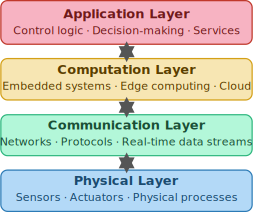
\includegraphics{cps_layers}
		\end{column}
	\end{columns}
\end{frame}

\begin{frame}[t]{CPS Application Domains}
	\begin{columns}
		\begin{column}{.5\linewidth}
			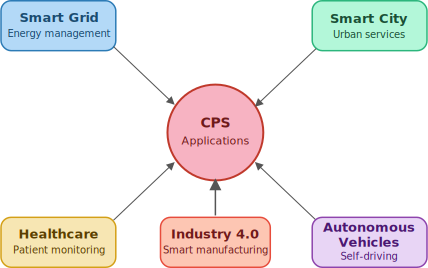
\includegraphics{cps_domains}
		\end{column}
		\begin{column}{.5\linewidth}
			\begin{compactdescription}
			\item[Smart Grid] demand-response, fault isolation
			\item[Smart City] traffic, waste, energy management
			\item[Healthcare] wearable monitors, surgical robots
			\item[Industry 4.0] flexible manufacturing, cobots
			\item[Autonomous Vehicles] perception-control loop
			\end{compactdescription}
			\begin{exampleblock}{Common Challenge}
				All domains require real-time decision-making in open,
				heterogeneous, and uncertain environments.
			\end{exampleblock}
		\end{column}
	\end{columns}
\end{frame}

\end{graphicspathcontext}

\endinput

	\subsection{Cyber-Physical System as Complex System}
	\begin{graphicspathcontext}{{./chapters/cps/imgs/},{./chapters/cps/imgs/auto/},\old}

\sidecite{Rajkumar2010CPS}
\begin{frame}{{Cyber-Physical Systems} as Complex Systems}
	\smaller
	\alertbox{Why Cyber-Physical Systems are intrinsically complex}
	\begin{columns}
		\begin{column}{.5\linewidth}
			\begin{compactitemize}
			\item Heterogeneous components (hardware + software)
			\item Continuous \emph{and} discrete dynamics (hybrid systems)
			\item Partial observability of the physical world
			\item Time constraints --- \emph{hard real-time} requirements
			\item Open environments --- components join/leave dynamically
			\end{compactitemize}
		\end{column}
		\begin{column}{.5\linewidth}
			\begin{compactitemize}
			\item Feedback loops induce \emph{non-linear} behaviour
			\item Failures cascade across layers
			\item Security and privacy at the cyber--physical interface
			\item Scale: from nano-sensors to city-wide infrastructure
			\end{compactitemize}
		\end{column}
	\end{columns}
	\vspace{.25cm}
	\begin{alertblock}{Consequence}
		Classical monolithic software architectures are \Emph{inadequate}. \\
		We need \Emph{decentralised, adaptive, autonomous} software entities that match the complexity of the physical world \\
		$\Rightarrow$ \Emph{Multiagent Systems for Cyber-Physical Systems}
	\end{alertblock}
\end{frame}

\end{graphicspathcontext}

\endinput

	\subsection{The Interplay: CPS, AI and MAS}
	\begin{graphicspathcontext}{{./chapters/cps/imgs/},{./chapters/cps/imgs/auto/},\old}

\sidecite{Baheti2011CPSImpact}
\begin{frame}{The Conceptual Landscape}
	\begin{columns}
		\begin{column}{.5\linewidth}
			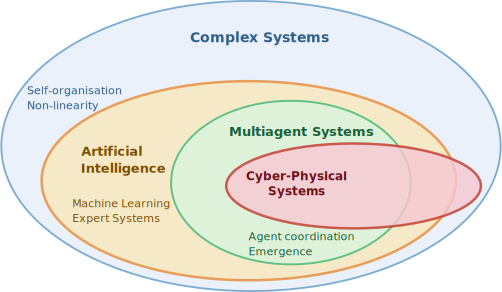
\includegraphics{cps_venn}
		\end{column}
		\begin{column}{.5\linewidth}
			\begin{description}
			\item[Complex Systems] provide the theoretical ground: emergence, self-organisation, non-linearity
			\item[Artifical Intelligence] provides the cognitive machinery: reasoning, learning, optimisation
			\item[Multiagent System] provides the architectural paradigm: decentralisation, coordination, autonomy
			\item[Cyber-Physical System] is the \emph{application domain} sitting at the intersection: it requires all three
			\end{description}
		\end{column}
	\end{columns}
\end{frame}

\sidecite{CossentinoGaudHilaireGallandKoukam2010_1}
\begin{frame}{Why MAS is the Right Model for CPS}
	\smaller
	\begin{columns}
		\begin{column}{.5\linewidth}
			\Emph{Mapping CPS requirements to MAS features:}
			\begin{stabularx}{X|X}
			\tabularhead{CPS Requirement}{MAS Answer} \\
			Distributed sensing      & Agent perception loop \\
			\hline
			Real-time reaction       & Reactive architecture \\
			\hline
			Goal-directed control    & BDI intentionality \\
			\hline
			Fault tolerance          & Agent redundancy \\
			\hline
			Openness                 & Dynamic agent population \\
			\hline
			Coordination             & Protocols \& contracts \\
			\hline
			Learning \& adaptation   & Reinforcement learning agents \\
			\end{stabularx}
		\end{column}
		\begin{column}{.5\linewidth}
			\begin{block}{Holonic MAS (HMAS)}
				Agents can be \emph{aggregated} into higher-level \Emph{holons}:
				\[
				h = (\{h_1, h_2, \dots, h_k\}, \{h_{k+1}, h_{k+2}, \dots, h_n\}, \dots)
				\]
				This naturally mirrors the \emph{hierarchical} layers of CPS
				(sensor $\rightarrow$ edge $\rightarrow$ cloud).
			\end{block}
			\begin{exampleblock}{SARL}
				The \emph{SARL} agent-oriented language provides:
				\begin{itemize}
				\item Capacities \& Skills
				\item Spaces \& Contexts
				\item Built-in BDI support
				\item Holonic agent model
				\end{itemize}
			\end{exampleblock}
		\end{column}
	\end{columns}
\end{frame}

\end{graphicspathcontext}

\endinput


	\section[MABS Examples]{Examples of Multiagent Systems}
	\subsection{Traffic on French Highway}
	\begin{graphicspathcontext}{{./chapters/simulation/examples/imgs/},{./chapters/simulation/examples/imgs/auto/},\old}

\begin{frame}{Highway Simulation}
	\begin{block}{What is simulated?}
		\begin{enumerate}
		\item Vehicles on a French highway.
		\item Danger event $\rightarrow$ ``an animal is crossing the highway and causes a crash''. 
		\item Alert events by GSM.
		\item Arrival of the security and rescue services.
		\end{enumerate}
	\end{block}
	\vfill
	\includegraphics[width=.6\linewidth]{uml_Aremis}\hfill\includegraphics[width=.25\linewidth]{voxelia2}
\end{frame}

\sidecite{GallandGaudDemangeKoukam2009_11}
\begin{frame}{Model of the Environment}
	\smaller
	\begin{block}{Road Network}
		\begin{itemize}
		\item Road polylines: $S = \left\{ \langle path, objects \rangle \big| path = \langle (x_0,y_0) \cdots \rangle \right\}$
		\item Graph: $G = \left\{ S, S \mapsto S, S \mapsto S \right\} = \left\{ \text{segments}, \text{entering}, \text{exiting} \right\}$
		\end{itemize}
	\end{block}
	\begin{block}{Operations}
		\begin{itemize}
		\item Compute the set of objects perceived by a driver (vehicles, roads...):
			\[P = \left\{ o \Bigg|
				\begin{matrix}
				distance(d,o)\le \Delta \wedge \\
				o \in O \wedge \\
				\forall (s_1,s_2), path = s_1.\langle p, O \rangle.s_2
				\end{matrix}
				\right\}\]
			where $path$ is the roads followed by a driver $d$
		\item Move the vehicles, and avoid physical collisions
		\end{itemize}
	\end{block}
\end{frame}

\begin{frame}[t]{{Driving} Model}
	\begin{columns}
		\begin{column}{.35\linewidth}
			\centering
			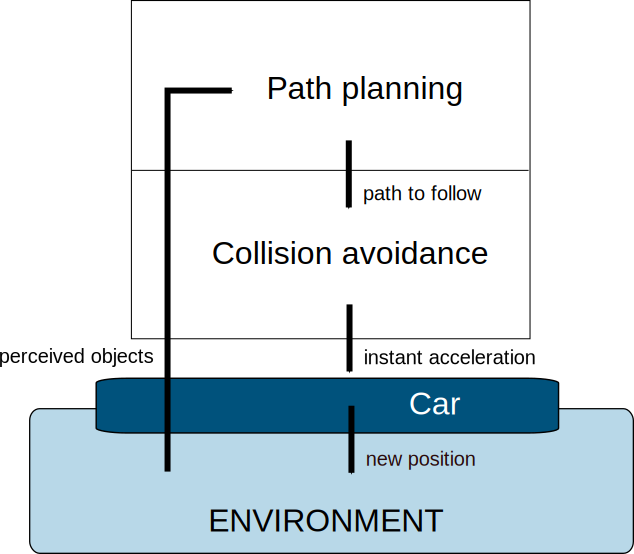
\includegraphics{carpooling_agent_layers}
			{\smaller\smaller\cite{GallandGaudDemangeKoukam2009_11}}
		\end{column}
		\begin{column}{.65\linewidth}
			\smaller
			\begin{block}{Path Planning}
			Based on the A* algorithm \cite{Dechter:1985:GBS:3828.3830,RoutePlanningAlgorithms2009} or D*-lite \cite{Koenig.Dstarlite.2005}
			\end{block}
			\begin{block}{Collision Avoidance}
				\begin{compactdescription}
				\item[Principle] compute the acceleration of the vehicle to avoid collisions with the other vehicles
				\item[Intelligent Driver Model] \cite{PhysRevE.62.1805}
				{\smaller
					\[acc = \begin{cases}
					- \dfrac{\left( v \Delta v \right)^2}{4b\Delta p^2} & \text{if the ahead object is far} \\
					- a \dfrac{\left( s + v w \right)^2}{\Delta p^2} & \text{if the ahead object is near} \\
					\end{cases}\]
				}
				\item[Free driving]
					{\smaller\[acc = a \left( 1 - \left(\frac{v}{v_c}\right)^4 \right)\]}
				\end{compactdescription}
			\end{block}
		\end{column}
	\end{columns}
\end{frame}

\begin{frame}[t,fragile]{Video of the French Highway Simulation}
	\vspace{-.25cm}
	\begin{center}
		\embeddedvideo[width=.8\linewidth]{./videos/simulation/aremis.avi}{aremis}
	\end{center}
	\begin{center}
		\tiny These videos were realized on the SIMULATE\textup{\regmark} tool \copyright Voxelia S.A.S
	\end{center}
\end{frame}

\end{graphicspathcontext}

\endinput


	\subsection{Pedestrian Simulation}
	\begin{graphicspathcontext}{{./chapters/simulation/examples/imgs/},{./chapters/simulation/examples/imgs/auto/},\old}

\begin{frame}{Pedestrian Simulation}
	\begin{block}{What is simulated?}
		\begin{enumerate}
		\item Movements of pedestrians at a microscopic level.
		\item Force-based model for avoiding collisions.
		\end{enumerate}
	\end{block}
	\vfill
	\cite{buisson.abmtrans13}\hfill\includegraphics[width=.25\linewidth]{voxelia2}
\end{frame}

\begin{frame}{Force to Apply to Each Agent}
	\begin{itemize}
	\item The force to apply to each agent is:\hfill\hbox to .2\linewidth{\vbox to 0pt {\includegraphicswtex[width=.2\linewidth]{pedestrian_agent_params}}}
		\[ \vec{F_a} = \vec{F} + w_a.\delta_{\|\vec{F}\|} \dfrac{\vec{p_t} - p_a}{\|\vec{p_t} - p_a\|} \]
		\[ \vec{F} = \sum_{i \in M} U(t_c^i) \cdot \hat{S_i} \]
	\item \smaller $\vec{F}$: collision-avoidance force.
	\item $\hat{S_i}$: a sliding force.
	\item $t_c^i$: time to collision to object $i$.
	\item $U(t)$: scaling function of the time to collision.
	\item $M$: set objects around (including the other agents).
	\item $w_a$: weight of the attractive force.
	\item $\delta_{x} g$: is $g$ if $x\leq0$, $0$ otherwise.
	\end{itemize}
\end{frame}

\begin{frame}{Sliding Force}
	\begin{itemize}
	\item The sliding force $\vec{S_i}$ is:
		\[ \vec{s_j} = (p_j - p_a) \times \hat{y} \]
		\[ \hat{S_j} = \sgn (\vec{s_j} \cdot (\vec{p_t} - p_a)) \frac{\vec{s_j}}{\|\vec{s_j}\|} \]
	\item \smaller $\hat{y}$: vertical unit vector.
	\end{itemize}
	\vfill
	\begin{center}
		\includegraphicswtex[width=.65\linewidth]{pedestrian_sliding_force}
	\end{center}
\end{frame}

\begin{frame}{Scaling the Sliding Force}
	\begin{itemize}
	\item \alert{How to scale $\hat{S_j}$ to obtain the repulsive force?}
	\item Many force-based models use a monotonic decreasing function of the distance to an obstacle.
	\item But it does not support the velocity of the agent.
	\vfill
	\item \alert{Solution: Use time-based force scaling function.}
		\[ U(t) = \begin{cases}
				\frac{\sigma}{{t}^\phi} - \frac{\sigma}{{t_{max}}^\phi} & \text{if }0\leq t\leq t_{max} \\
				0 & \text{if }t > t_{max}
			\end{cases} \]
	\item \smaller $t$: estimated time to collision.
	\item $t_{max}$: the maximum anticipation time.
	\item  $\sigma$ and $\phi$ are constants, such that $U(t_{max}) = 0$.
	\end{itemize}
\end{frame}

\begin{frame}[t,fragile]{{Video 1:} Collision Avoidance Behavior}
	\vspace{-.25cm}
	\begin{center}
		\embeddedvideo[width=.52\linewidth]{./videos/simulation/pedestrians_circle.avi}{pedestrians_circle}
			\\
	\tiny This video was realized on the SIMULATE\textup{\regmark} tool \copyright Voxelia S.A.S
	\end{center}
\end{frame}

\begin{frame}[t,fragile]{{Video 2:} Simulation of Belfort Railway Station}
	\vspace{-.2cm}
	\begin{center}
		\embeddedvideo[width=.9\linewidth]{./videos/simulation/pedestrians_gare_belfort.avi}{pedestrians_gare_belfort}
		\\
		\tiny This video was realized on the SIMULATE\textup{\regmark} tool \copyright Voxelia S.A.S
	\end{center}
\end{frame}

\begin{frame}[t,fragile]{{Video 3:} Simulation of Belfort Downtown}
	\vspace{-.2cm}
	\begin{center}
		\embeddedvideo[width=.8\linewidth]{./videos/simulation/pedestrians_place_arme_belfort.avi}{pedestrians_place_arme_belfort}
		\\
		\tiny This video was realized on the SIMULATE\textup{\regmark} tool \copyright Voxelia S.A.S
	\end{center}
\end{frame}

\begin{frame}[t,fragile]{{Video 4:} Drone Behavior}
	\vspace{-.2cm}
	\begin{center}
		\embeddedvideo[width=.9\linewidth]{./videos/simulation/pedestrians_drones.mp4}{pedestrians_drones_sarl}
		\\
		\tiny This video was realized with SARL and Airsim
	\end{center}
\end{frame}

\end{graphicspathcontext}

\endinput


	\subsection{Digital Twin of an Autonomous Vehicle}
	\begin{graphicspathcontext}{{./chapters/simulation/examples/imgs/},{./chapters/simulation/examples/imgs/auto/},\old}

\begin{frame}{Autonomous Vehicle}
	\begin{columns}[c]
		\begin{column}{.6\linewidth}
			\begin{block}{Autonomous Vehicle}
			\begin{itemize}
			\item perceiving its environment: video, laser and GPS sensors
			\item driving by itself, or taking control in urgency cases
			\end{itemize}
			\end{block}
			\begin{block}{Goals}
			\begin{enumerate}
			\item Simulate the \Emph{driver behavior}
			\item Simulate the environment and the \Emph{sensors} in a virtual lab
			\item \Emph{Deploy the driver software} in the real vehicles without change
			\end{enumerate}
			\end{block}
		\end{column}
		\begin{column}{.39\linewidth}
			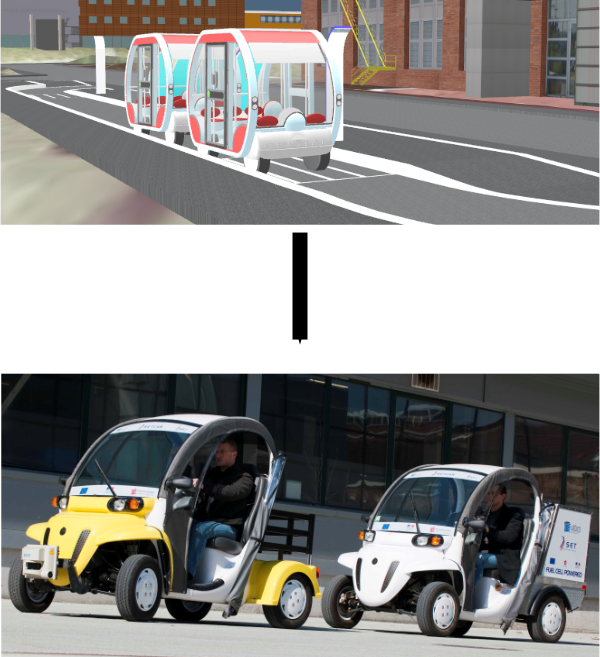
\includegraphics[width=\linewidth]{vivus_setcar}
		\end{column}
	\end{columns}
\end{frame}

\begin{frame}{Video of the Simuled and Real Systems}
	\vspace{-.5cm}
	\begin{center}
		\embeddedvideo[width=.65\linewidth]{./videos/simulation/autonomousvehicle_setcar.mp4}{autonomousvehicle_setcar}
		\\
		\cite{gechter12}
	\end{center}
\end{frame}

\end{graphicspathcontext}

\endinput



	\thanksslide
\end{bibliographysection}

\part{Introduction to Multiagent Systems}
\begin{bibliographysection}

	\section{Agent}
	\begin{graphicspathcontext}{{./chapters/mas/imgs/},{./chapters/mas/imgs/auto/},\old}

\begin{frame}{Agent: a first definition}
	\begin{definitionblock}{Agent \cite{Wooldridge09}}
		An agent is an entity with (at least) the following attributes/characteristics:
		\begin{enumerate}
		\item Autonomy
		\item Interaction - Social Skills - Sociability
		\item Reactive behavior
		\item Proactive behavior
		\end{enumerate}
	\end{definitionblock}
	\vspace{.5cm}	
	\hiconbox*{No commonly/universally accepted definition}{info-icon}
\end{frame}

\begin{frame}[t]{Agent: Autonomy}
	\begin{columns}
		\begin{column}{.2\linewidth}
			\begin{bottomarrowsequence}
				\arrow[bg=CIADgreen]{Autonomy}
				\arrow{Interaction}
				\arrow{Reactive}
				\arrow{Proactive}
			\end{bottomarrowsequence}
		\end{column}
		\begin{column}{.8\linewidth}
			\begin{definitionblock}{Principle of autonomy}
				Agents encapsulate their \Emph{internal state} (that is not accessible to other agents), and make decisions about what to do based on this state, without the direct intervention of humans or others agent
			\end{definitionblock}
			\vspace{.5cm}
			\begin{itemize}
				\item Able to \alert{act without any direct intervention} of human users or other agents
				\item Total \alert{control} over its own \alert{internal state}
				\item Total \alert{control} over its own \alert{actions} (no master/slave relationship)
				\item Can modify its behavior according to its experience (\alert{adaptation} or \alert{learning})
			\end{itemize}
		\end{column}
	\end{columns}
\end{frame}

\begin{frame}[t]{Agent: Interaction}
	\vspace{-.5cm}
	\begin{columns}
		\begin{column}[t]{.2\linewidth}
			\begin{bottomarrowsequence}
				\arrow{Autonomy}
				\arrow[bg=CIADgreen]{Interaction}
				\arrow{Reactive}
				\arrow{Proactive}
			\end{bottomarrowsequence}
		\end{column}
		\begin{column}[t]{.8\linewidth}
			\only<1>{
				\begin{definitionblock}{Principle of interaction}
					Agent interacts with other agents, and have the ability to engage in social activities (cooperation, coordination, negotation...) in order to achieve its goals
				\end{definitionblock}
				\begin{itemize}
				\item \Emph{The whole is greater than the sum of its parts}
				\item Require a mechanism to exchange information
				\item Many tasks can only be done by:
					\begin{description}
					\item[Cooperation] Agents work together toward a shared goal, often by sharing resources or information to achieve mutual benefit
					\item[Coordination] Agents organize their actions and interactions to avoid conflicts, ensure efficiency, and align with system objectives
					\item[Negotiation] Agents engage in communication and bargaining to resolve conflicts, allocate tasks, or reach agreements on actions or resource use
					\end{description}
				\end{itemize}
			}
			\only<2->{
				\begin{columns}
					\begin{column}[t]{.5\linewidth}
						\fancybox[width=5.2cm]{Direct Interaction}{
							\Emph{Peer-to-peer communication} \\
							Direct, bilateral, and explicit addressing
						}{direct-agent-interaction}{}
					\end{column}
					\begin{column}[t]{.5\linewidth}
						\fancybox[width=5.7cm]{Indirect Interaction}{
							\Emph{Stigmergy: interact without direct contact through the environment} \\
							Deposit persistent traces,
							Perceive and react to traces
						}{indirect-agent-interaction}{}
					\end{column}
				\end{columns}
				\begin{center}
					\only<2>{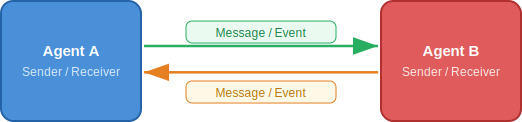
\includegraphics[width=.6\linewidth]{direct_interaction}}
					\only<3>{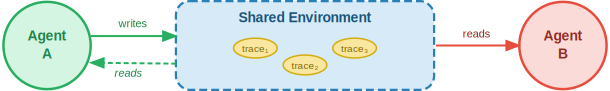
\includegraphics[width=.7\linewidth]{indirect_interaction}}
				\end{center}
			}
		\end{column}
	\end{columns}
\end{frame}

\begin{frame}[t]{Agent: Reactive Behavior}
	\vspace{-.5cm}
	\begin{columns}
		\begin{column}[t]{.2\linewidth}
			\begin{bottomarrowsequence}
				\arrow{Autonomy}
				\arrow{Interaction}
				\arrow[bg=CIADgreen]{Reactive}
				\arrow{Proactive}
			\end{bottomarrowsequence}
		\end{column}
		\begin{column}[t]{.8\linewidth}
			\begin{definitionblock}{Principle of reactive behavior}
				Agent \Emph{perceives} its environment and \Emph{immediately produces an action in response}, without planning or memory
			\end{definitionblock}
			\begin{description}
			\item[Perception $\rightarrow$ Action] behavior is a direct mapping from sensed stimuli to output actions
			\item[No internal model] agent holds no representation of the world
			\item[No deliberation] no reasoning, planning, or goal inference occurs
			\item[Quick response] reaction is immediate and computationally lightweight
			\item[Emergence] complex collective behaviors can arise from many simple reactive agents
			\end{description}
		\end{column}
	\end{columns}
\end{frame}

\begin{frame}[t]{Agent: Proactive Behavior}
	\vspace{-.5cm}
	\begin{columns}
		\begin{column}[t]{.2\linewidth}
			\begin{bottomarrowsequence}
				\arrow{Autonomy}
				\arrow{Interaction}
				\arrow{Reactive}
				\arrow[bg=CIADgreen]{Proactive}
			\end{bottomarrowsequence}
		\end{column}
		\begin{column}[t]{.8\linewidth}
			\begin{definitionblock}{Principle of proactive behavior}
				Agent \Emph{pursues its own goals} by anticipating future states and planning actions, independently of immediate stimuli
			\end{definitionblock}
			\begin{description}
			\item[Goal-driven] behavior is directed by internal objectives, not just external stimuli
			\item[Internal model] agent maintains a representation of the world to reason about it
			\item[Deliberation] agent evaluates options and selects actions toward its goals
			\item[Anticipation] agent predicts future states to plan ahead
			\item[Initiative] the agent acts on its own, without waiting for external triggers
			\end{description}
		\end{column}
	\end{columns}
\end{frame}

\sidenote{\cite{Ferber.1999,Weyns05,Michel.07}, Claude Sonnet 4.6}
\figureslide{{Agent and Agent Environment} in Multiagent Systems}{agentenvironment}

\begin{frame}[t]{{Some Questions} about the Agent Environment}
	\vspace{-.1cm}
	\begin{center}
		\begin{bottomarrowsequence}
			\arrow[bg=CIADlightgray,fg=CIADdarkgray]{What is included in the agent environment?}
			\arrow[bg=CIADdarkgray,fg=white]{Are all agent situated in the agent environment?}
			\arrow[bg=black,fg=white]{What is the the body of the agent and where is it localized?}
		\end{bottomarrowsequence}
	\end{center}
\end{frame}

\sidecite{Saunier2015}
\figureslide{Agent Body}{body_mind}

\begin{frame}{Agent: another definition}
	\footnotesize{
		\begin{definitionblock}{Agent \cite{Ferber.1999}}
			Agent is a virtual (software) or physical entity which:
			\begin{itemize}
			\item is capable of acting in an environment
			\item can communicate directly with other agents
			\item is driven by a set of tendencies (in the form of individual objectives or of a satisfaction/survival function which it tries to optimize)
			\item possesses resources of its own
			\item is capable to perceive its environment, but up to a limited extent
			\item has only a partial representation of this environment and perhaps none at all
			\item possesses skills and can offer services
			\item may be able to reproduce itself
			\item whose behavior tends towards satisfying its objectives, taking account of the resources and skills available to it and depending on its perception, its representation and the communication it receives
			\end{itemize}
		\end{definitionblock}
	}
\end{frame}

\begin{frame}{{Other Properties} for Agents}
	\smaller
	\begin{stabularx}{c|X|c}
	\tabularhead{Property}{Explanation}{Reference} \\
	Mobility & Move through different nodes of a network/grid & \tiny\cite{OKeefe98} \\
	\hline
	Adaptability & Modify the actions/behavior according to external conditions and perceptions & \tiny\cite{Weiss.99} \\
	\hline
	Versatility & Ability to perform different tasks or to meet different objectives & \tiny\cite{roadmapagentresearchdevel} \\
	\hline
	Trustiness & Level of confidence that inspires the agent to delegate tasks, perform action, collaborate with other agents & \tiny\cite{Sabater05} \\
	\hline
	Robustness & Continue to operate in fault situations, even with lower performances & \tiny\cite{Shehory98} \\
	\hline
	Persistence & Keep continuously running by retrieving or saving their internal state even after a crash or unexpected situations & \tiny\cite{Weiss.99} \\
	\hline
	Altruism & Disposition of an agent to assist other agents in their tasks & \tiny\cite{Castelfranchi98} \\
	\end{stabularx}
\end{frame}

%\begin{frame}{Agent vs. Object}
%	\begin{block}{Agent vs Object~\cite{Wooldridge.01.survey}}
%		\begin{itemize}
%		\item Agents are autonomous, they decide on the execution of services: ``\alert{\textit{Objects do it for free; agents do it because they want to}}''.
%		\item The agents allow flexible (reactive, pro-active, social) and autonomous behavior.
%		\item MAS are inherently ``multi-thread''. Each agent has its own thread of execution.
%		\end{itemize}
%	\end{block}
%\end{frame}



%\begin{frame}{Agent vs. Expert System}
%	\begin{block}{Key Differences}
%		An Expert System (ES) maintains various \alert{facts} about the world that are used to draw \alert{conclusions}.
%	\end{block}

%	\begin{block}{Key Differences}
%		\begin{itemize}
%		\item Traditional ES are not situated in an environment. There is no direct coupling with the environment and requires a user that acts as an intermediary ue.
%		\item ES are usually not capable of exhibiting flexible behavior (reactive and proactive).
%		\item ES are usually not provided with social skills (communication and interaction with other agents).
%		\end{itemize}
%	\end{block}
%\end{frame}

\end{graphicspathcontext}

\endinput



	\section{Multiagent System}
	\begin{graphicspathcontext}{{./chapters/mas/imgs/},{./chapters/mas/imgs/auto/},\old}

\begin{frame}{{Two perspectives} on Agent-based Systems}
	\begin{columns}
		\begin{column}{.5\linewidth}
			\centering
			\fancybox[width=7cm,bg=CIADdarkgray]{Mono-Agent Approach}{
				\Emph{System composed of a single agent} \\
				Example: personal assistant
			}{monoagent-system}{1}
		\end{column}
		\begin{column}{.5\linewidth}
			\centering
			\fancybox[width=7cm]{Multi-Agent Approach}{
				\Emph{System composed of multiple agents} \\
				Global or collective task is built from agent actions \\
				Result \emph{emerges} from the local interactions and behaviors
			}{multiagent-system}{+}
		\end{column}
	\end{columns}
\end{frame}

\begin{frame}{{Multiagent System:} a first definition}
	\begin{definitionblock}{Multiagent System \cite{Wooldridge09}}
	Multi-agent system is a system composed of multiple interacting intelligent agents, where each agent has incomplete information or capabilities to solve a problem and thus must interact with others to achieve its goals or the system's goals
	\end{definitionblock}
\end{frame}

\sidenote{Images by Claude Sonnet 4.6}
\begin{frame}{Interaction in Multiagent Systems}
	\begin{description}
		\item[Direct Interaction] \raisebox{-.4\height}{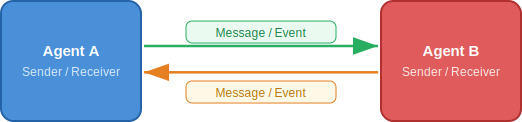
\includegraphics[width=.6\linewidth]{direct_interaction}}
		\vspace{.5cm}
		\item[Indirect Interaction] \raisebox{-.4\height}{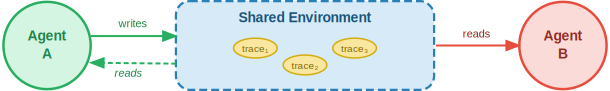
\includegraphics[width=.7\linewidth]{indirect_interaction}}
	\end{description}
	\begin{columns}
		\begin{column}[t]{.5\linewidth}
			\begin{definitionblock}{Stigmergy in biology \cite{Grasse59}}
				Form of self-organization in which the trace left in the environment by an action stimulates the performance of a subsequent action, either by the same entity or by other entities
			\end{definitionblock}
		\end{column}
		\begin{column}[t]{.5\linewidth}
			\begin{definitionblock}{Stigmergy in MAS \cite{Dorigo92}}
				Agents interact by modifying a shared environment and these modifications influence the subsequent actions of the same or other agents
			\end{definitionblock}
		\end{column}
	\end{columns}
\end{frame}

\begin{frame}{{Multiagent System:} another definition}
	\begin{definitionblock}{Multiagent System \cite{Ferber.1999}}
		System comprising the following elements: 
		\begin{itemize}
		\item An environment E, usually a space (may be with volume, 3D)
		\item An array of objects, $O$. These objects are situated
		\item A set of agents, $A$, which are specific objects
		\item A set of relations, $R$, which links the objects (and thus agents)
		\item A set of operations, $Op$, making it possible for agents to receive, produce, process and manipulate the objects in $O$
		\item Operators with the task of representing the application of these operations and the reaction of the world to this attempt of modification
		\end{itemize}
	\end{definitionblock}
\end{frame}

\begin{frame}[t]{Modeling from Local to Global}
	\vspace{-.25cm}
	\hiconbox{
		\Emph{Individual level:} design each agent model
		\begin{description}
		\item[Agent architecture] internal decision process based on reactive or proactive mechanisms
		\item[Autonomy level] delegate tasks to agent capacities, resources or the operating system
		\end{description}
	}{monoagent-system}
	\hiconbox{
		\Emph{Society level:} choose the global mechanisms
		\begin{description}
		\item[Hierarchy] is and how agent composed by other agent?
		\item[Decentralization] how control is distributed other agents, who has authority? (social pattern, norms)
		\item[Agreement technologies] how to coordinate, cooperate, negotiate?
		\item[Emergence] how to implement and influence emergence?
		\item[Distribution] how agents are physically distribued?
		\end{description}
	}{multiagent-system}
\end{frame}

\end{graphicspathcontext}

\endinput



	\section{Basic Examples}
	\subsection{Vaacum Robot}
	\begin{graphicspathcontext}{{./chapters/mas/examples/imgs/auto/},\old}

\sidenote{\cite{Russell.20}, Image Clause Sonet 4.6}
\begin{frame}{Definition of the Vacuum World}
	\begin{columns}
		\begin{column}[t]{.5\linewidth}
			\begin{block}{Environment}
				\begin{itemize}
				\item A grid of \emph{rooms}, each of which is either \emph{Clean} or \emph{Dirty}
				\item One (or more) \emph{vacuum robot(s)} occupying a room at a time
				\end{itemize}
			\end{block}
			\begin{block}{Agent}
				\begin{description}
				\item[Perceives] \texttt{Dirty}, \texttt{Clean}, \texttt{CanGoLeft}, \texttt{CanGoRight}, \texttt{CanGoUp}, \texttt{CanGoDown}
				\item[Acts] \texttt{Suck}, \texttt{MoveLeft}, \texttt{MoveRight}, \texttt{MoveUp}, \texttt{MoveDown}
				\end{description}
			\end{block}
		\end{column}
		\begin{column}[t]{.5\linewidth}
			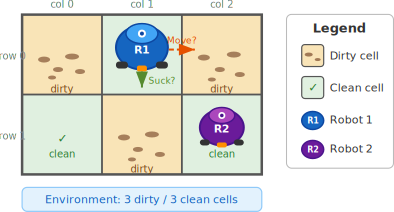
\includegraphics{vacuum_world} \\[.5cm]
			\begin{block}{Possible Performance Measure}
			Maximise the \emph{number of clean cells} over time, minimising energy consumption
			\end{block}
		\end{column}
	\end{columns}
\end{frame}

\begin{frame}[fragile]{Vacuum Agent Loop}
	\begin{columns}
		\begin{column}{.5\linewidth}
				\begin{sarllisting}
def run() {
	var done = false
	while (!done) {
	  var p = get_percept()
	  var a = choose_action(p)
	  do_action(a)
	  done = check_if_done()
	}
	die()
}\end{sarllisting}
		\end{column}
		\begin{column}{.5\linewidth}
			\begin{block}{\texttt{get\_percept()}}
				Convert sensor data to the logical facts for perceptions
			\end{block}
			\begin{block}{Reactive behavior: \texttt{choose\_action()}}
				If the current cell is dirty, suck \\
				Otherwise, move \\[1ex]
				\centering
				\begin{tabular}{|c|c|}
				\hline
				\textbf{Perception \texttt{p}} & \textbf{Action \texttt{a}} \\
				\hline
				\texttt{[Dirty]} & \texttt{Suck} \\
				\hline
				\texttt{[Clean, CanGoLeft]} & \texttt{MoveLeft} \\
				\hline
				\texttt{[Clean, CanGoRight]} & \texttt{MoveRight} \\
				\hline
				\texttt{[Clean, CanGoUp]} & \texttt{MoveUp} \\
				\hline
				\texttt{[Clean, CanGoDown]} & \texttt{MoveDown} \\
				\hline
				\end{tabular}
			\end{block}
		\end{column}
	\end{columns}
\end{frame}

\begin{frame}[fragile]{Vacuum Agent Loop \insertcontinuationtext}
	\begin{columns}
		\begin{column}{.5\linewidth}
				\begin{sarllisting}
def run() {
	var done = false
	while (!done) {
	  var p = get_percept()
	  var a = choose_action(p)
	  do_action(a)
	  done = check_if_done()
	}
	die()
}\end{sarllisting}
		\end{column}
		\begin{column}{.5\linewidth}
			\begin{block}{\texttt{do\_action()}}
				Convert selected action fact to a concrete effect with the robot effectors
			\end{block}
			\begin{block}{\texttt{check\_if\_done()}}
				Determine if the robot has to stop its running
			\end{block}
			\begin{block}{Does this agent perform well?}
				\smaller Need a performance measure:
				\begin{compactitemize}
				\item Maximize amount of dirt picked up?
				\item Maximize ratio of dirt to energy expended?
				\item Maximize ratio of dirt to combination of energy and time?
				\end{compactitemize}
				Selecting a performance measure is not always easy
			\end{block}
		\end{column}
	\end{columns}
\end{frame}

\end{graphicspathcontext}

\endinput


	\subsection{Forager Bots}
	\begin{graphicspathcontext}{{./chapters/mas/examples/imgs/auto/},\old}

\sidenote{\cite{Ferber.1999}, Image Clause Sonet 4.6}
\begin{frame}[t]{Forager Bots}
	\begin{block}{Scenario \cite{Ferber.1999}}
		\smaller A colony of \emph{autonomous robots} (bots) operates in a shared environment.
		Their collective goal is to \emph{gather food items} scattered across the environment and bring them back to a central \emph{nest (base camp)}
	\end{block}
	\begin{columns}
		\begin{column}{.5\linewidth}
			\begin{block}{Key Elements}
				\begin{description}
					\item[Agents] forager bots
					\item[Environment] a 2-D grid or continuous space
					\item[Resources] food items spread randomly
					\item[Base] nest where food is deposited
				\end{description}
			\end{block}
		\end{column}
		\begin{column}{.5\linewidth}
			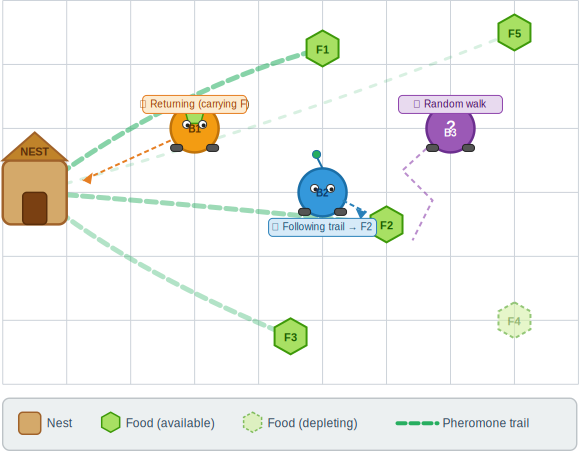
\includegraphics{forager_bots}
		\end{column}
	\end{columns}
\end{frame}

\begin{frame}[fragile]{Forager Agent Loop}
	\begin{columns}
		\begin{column}{.5\linewidth}
				\begin{sarllisting}
def run() {
	var done = false
	while (!done) {
	  var p = get_percept()
	  var a = choose_action(p)
	  do_action(a)
	  done = check_if_done()
	}
	die()
}\end{sarllisting}
		\end{column}
		\begin{column}{.5\linewidth}
			\smaller
			\begin{block}{\texttt{get\_percept()}}
				\begin{compactdescription}
				\item[Sense nearby cells] food present? pheromone level? other bots?
				\item[Read internal state] \emph{carrying food?} current position
				\end{compactdescription}
			\end{block}
			\begin{block}{\texttt{do\_action()}}
				\begin{compactdescription}
				\item[Move] to an adjacent cell (towards food or towards nest)
				\item[Pick up] a food item (if on a food cell and not loaded)
				\item[Drop] food at the nest (if carrying and at nest)
				\item[Deposit pheromone] on the current cell
				\item[Update internal state] toggle \texttt{carrying\_food} flag; update position
				\end{compactdescription}
			\end{block}
		\end{column}
	\end{columns}
\end{frame}

\begin{frame}{Forager Decision Process}
	\begin{columns}
		\begin{column}{.5\linewidth}
			\begin{block}{Mode 1 --- Foraging}
				\Emph{Constraint:} Bot is \emph{not} carrying food \\
				\Emph{Goal:} find a food item \\
				\Emph{Strategy:}
				\begin{itemize}
				\item If food is visible $\Rightarrow$ move to food \& pick it up
				\item Else if pheromone trail nearby $\Rightarrow$ follow trail
				\item Else $\Rightarrow$ random walk (exploration)
				\end{itemize}
			\end{block}
		\end{column}
		\begin{column}{.5\linewidth}
			\begin{block}{Mode 2 --- Returning}
				\Emph{Constraint:} Bot \emph{is} carrying food \\
				\Emph{Goal:} bring food to the nest \\
				\Emph{Strategy:}
				\begin{itemize}
				\item Navigate back towards the nest (gradient / memory)
				\item Deposit pheromone on the path (positive feedback)
				\item Drop food when reaching the nest
				\end{itemize}
			\end{block}
		\end{column}
	\end{columns}
\end{frame}

\sidenote{Image by Claude Sonnet 4.6}
\figureslide{Forager Flow Chart}{forager_bots_flowchart}

\begin{frame}{Emergent Behaviour}
	\begin{block}{Stigmergy}
	Bots communicate \Emph{indirectly} through the environment via pheromone
	trails.  No bot has global knowledge; yet the colony collectively discovers
	and exploits food sources efficiently.
	\end{block}
	\bigskip
	\Emph{Emergent properties observed:}
	\begin{description}
	\item Shortest paths to food are reinforced (pheromone accumulates faster)
	\item Exhausted food sources are naturally abandoned (trail evaporates)
	\item The system is \Emph{robust}: losing one bot does not break the colony
	\item[Scalability] adding more bots increases throughput without redesigning any individual agent.
	\end{description}
\end{frame}

\end{graphicspathcontext}

\endinput



	\section{Interests of Multiagent Systems}
	\begin{graphicspathcontext}{{./chapters/mas/imgs/},{./chapters/mas/imgs/auto/},\old}

\begin{frame}[t]{Interests for Using Multiagent Systems}
	\vspace{-.51cm}
	\begin{columns}
		\begin{column}[t]{.2\linewidth}
			\begin{bottomarrowsequence}
				\only<1>{\arrow[bg=CIADgreen]{Natural}}
				\only<2->{\arrow{Natural}}
				\only<2>{\arrow[bg=CIADgreen]{Distribution}}
				\only<1,3->{\arrow{Distribution}}
				\only<3>{\arrow[bg=CIADgreen]{Heterogeneity}}
				\only<1-2,4->{\arrow{Heterogeneity}}
				\only<4>{\arrow[bg=CIADgreen]{Openness}}
				\only<1-3,5->{\arrow{Openness}}
				\only<5>{\arrow[bg=CIADgreen]{Complexity}}
				\only<1-4,6->{\arrow{Complexity}}
				\only<6>{\arrow[bg=CIADgreen]{Legacy}}
				\only<1-5>{\arrow{Legacy}}
			\end{bottomarrowsequence}
		\end{column}
		\begin{column}[t]{.8\linewidth}
			\only<1>{
				\simplebox{``For many problems, the agent metaphor provides an \emph{intuitive and natural way of thinking} about, designing and implementing complex software systems'' \cite{Wooldridge09}}
				\begin{columns}
					\begin{column}{.5\linewidth}
						\begin{block}{Why?}
							\smaller
							\begin{itemize}
							\item Many real-world problems already involve
							\emph{independent, interacting entities}
							\item Agents \emph{mirror} real-world actors
							\item Decomposing a problem into agents
							\emph{matches the domain structure}
							directly, reducing the abstraction gap
							\item Stakeholders can reason using familiar concepts
							\end{itemize}
						\end{block}
					\end{column}
					\begin{column}{.5\linewidth}
						\viconbox{
							\smaller
							\begin{description}
								\item[Easier modelling] one-to-one mapping
								\item[Maintainability] changes translate naturally
								\item[Communicability] stakeholders
								understand
								\item[Scalability] new real-world
								actors $\Rightarrow$ new agents
							\end{description}
						}{pros-icon}
					\end{column}
				\end{columns}
			}
			\only<2>{
				\simplebox{``Some problems are most naturally seen as a collection of independent, autonomous components that must \emph{coordinate} to achieve a goal, where there is \emph{no single locus of control} and data may be \emph{inherently distributed}'' \cite{Wooldridge09}}
				\begin{columns}
					\begin{column}{.5\linewidth}
						\begin{block}{Why?}
							\smaller
							\begin{compactitemize}
								\item Many real systems have \emph{no natural central authority}
								\item Data is often \emph{physically or legally impossible to centralize}
								\item Single controller $=$ failure or performance bottleneck
								\item Reducing latency with \emph{local and autonomous} actions
								\item Coordination emerges local interactions
							\end{compactitemize}
						\end{block}
					\end{column}
					\begin{column}{.5\linewidth}
						\viconbox{
							\smaller
							\begin{compactdescription}
								\item[Fault tolerance] other agents continue operating
								\item[Scalability] new agent $\Rightarrow$ no redesigning
								\item[Privacy preservation] only local data
								\item[Parallelism] agents act simultaneously
								\item[Responsiveness] local decisions reduce response overhead
							\end{compactdescription}
						}{pros-icon}
					\end{column}
				\end{columns}
			}
			\only<3>{
				\simplebox{``Multiagent systems are a natural paradigm for building systems that integrate \emph{heterogeneous} components, possibly developed independently, using different languages, architectures, or data representations, [...]'' \cite{Wooldridge09}}
				\begin{columns}
					\begin{column}{.5\linewidth}
						\begin{block}{Why?}
							\smaller
							\begin{compactitemize}
								\item Systems with \emph{independently developed} components
								\item Agents have \emph{different architectures}
								\item Agents pursue \emph{different objectives}
								\item Data in \emph{different formats, ontologies, or protocols}
								\item \emph{No single model} fits all sub-problems
								\item Agents implemented with \emph{different technologies}
							\end{compactitemize}
						\end{block}
					\end{column}
					\begin{column}{.5\linewidth}
						\viconbox{
							\smaller
							\begin{compactdescription}
								\item[Specialisation] optimised agent for specific task
								\item[Emergent capabilities] combining agents with complementary behaviours
								\item[Standardised interaction] common communication protocols allow heterogeneous agents to coordinate transparently
							\end{compactdescription}
						}{pros-icon}
					\end{column}
				\end{columns}
			}
			\only<4>{
				\simplebox{``In an \emph{open} multiagent system, agents can freely enter and leave the system at runtime. The system does not assume a \emph{fixed, pre-known} set of participants, unlike \emph{closed} systems where all components are determined at design time'' \cite{Wooldridge09}}
				\begin{columns}
					\begin{column}{.5\linewidth}
						\begin{block}{Why?}
							\smaller
							\begin{compactitemize}
								\item Many systems are \emph{inherently dynamic}
								\item \emph{Impossible to enumerate} all future participants
								\item Closed systems \emph{break} when adding or removing component
								\item Open systems reflect the \emph{social and organisational} nature of real-world interactions
								\item Openness enables \emph{incremental deployment}
							\end{compactitemize}
						\end{block}
					\end{column}
					\begin{column}{.5\linewidth}
						\viconbox{
							\smaller
							\begin{compactdescription}
								\item[Dynamic scalability] no system restart
								\item[Self-organisation] system adapts its structure
								\item[Evolvability] system can incorporate new capabilities
								\item[Resilience] departing or failing agents do not halt the system
							\end{compactdescription}
						}{pros-icon}
					\end{column}
				\end{columns}
			}
			\only<5>{
				\simplebox{``Agent-oriented approaches provide an \emph{adequate paradigm} for the modelling of complex systems, since a complex system can be naturally described as a \emph{society of interacting autonomous agents}, exhibiting emergent behaviour, self-organisation, and decentralised control at multiple levels of abstraction.'' \cite{CossentinoGaudHilaireGallandKoukam2010_1}}
				\begin{columns}
					\begin{column}{.5\linewidth}
						\begin{block}{Why?}
							\smaller
							\begin{compactitemize}
								\item Complex systems consist of many
								\emph{interacting autonomous entities}
								whose global behaviour \emph{emerges}
								from local interactions
								\item \emph{No central controller}
								\item \emph{Autonomy,
								reactivity, proactivity, social ability} of complex entities \cite{Wooldridge95}
								\item \emph{Multilevel structure} of complex systems \cite{Holland.95}
							\end{compactitemize}
						\end{block}
					\end{column}
					\begin{column}{.5\linewidth}
						\viconbox{
							\smaller\smaller
							\begin{compactdescription}
								\item[Emergence] system behaviour from nonlinear interactions
								\item[Self-organisation] agents dynamically restructure their interactions
								\item[Scalability] Huge number of entities
								\item[Hierarchy] systems decomposed into complex systems
								\item[Decentralised control] complex systems are intrinsically parallel
							\end{compactdescription}
						}{pros-icon}
					\end{column}
				\end{columns}
			}
			\only<6>{
				\simplebox{\smaller ``Perhaps the most persuasive argument for agent-based computing is the \emph{legacy system} argument. Many organisations have a \emph{large investment} in software that cannot simply be discarded. The agent metaphor provides a natural way of \textbf{wrapping} these legacy components so that they can interact with newer systems'' \cite{Wooldridge09}}
				\begin{columns}
					\begin{column}{.5\linewidth}
						\begin{block}{Why?}
							\smaller
							\begin{compactitemize}
								\item Organisations accumulate \emph{decades
								of software investment} with \emph{critical business logic}
								\item Connecting legacy systems to modern architectures creates \emph{tight coupling}
								\item \emph{Interoperability} between heterogeneous legacy systems and modern services is a fundamental enterprise challenge
							\end{compactitemize}
						\end{block}
					\end{column}
					\begin{column}{.5\linewidth}
						\viconbox{
							\smaller
							\begin{compactdescription}
								\item[Agent wrapping] legacy system encapsulated behind agent
								\item[Incremental migration] from legacy system to agents progressively
								\item[Reusability] legacy system becomes reusable service to agents
							\end{compactdescription}
						}{pros-icon}
					\end{column}
				\end{columns}
			}
  		\end{column}
	\end{columns}
\end{frame}

\end{graphicspathcontext}

\endinput



	\thanksslide
\end{bibliographysection}

\part{Agent-Oriented Programming}
\begin{bibliographysection}

	\section{Bases of Agent-Oriented Programming}
	\begin{graphicspathcontext}{{./chapters/mas/imgs/},{./chapters/mas/imgs/auto/},\old}

\begin{frame}{Why Go Beyond Objects?}
	\begin{columns}
		\begin{column}[t]{.5\linewidth}
			\begin{block}{Object-Oriented Programming}
				\begin{itemize}
				\item Passive entities called by others
				\item No autonomous decision-making
				\item No perception of the world
				\item No explicit notion of goals
				\item Concurrency is ad-hoc
				\end{itemize}
			\end{block}
			\vspace{.5cm}
			\centering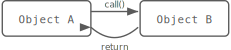
\includegraphics[width=.8\linewidth]{oop}
		\end{column}
		\begin{column}[t]{.5\linewidth}
			\begin{block}{Agent-Oriented Programming}
				\begin{description}
				\item[Autonomous] acts on its own initiative
				\item[Proactive] pursues goals
				\item[Reactive] responds to the environment
				\item[Social] interacts with other agents
				\item Concurrency is \emph{native}
				\end{description}
			\end{block}
			\vspace{.5cm}
			\centering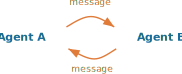
\includegraphics[width=.7\linewidth]{aop}
		\end{column}
	\end{columns}
\end{frame}

\figureslide{Levels of Abstraction in Software}{aop_abstraction_levels}

\figureslide{{Sense-Decide-Act} Loop}{aop_agent_loop}

\begin{frame}[t]{Several Agent Programming Languages and Frameworks}
	\vspace{-.3cm}
	\scriptsize
	\begin{stabularx}{X|c|c|c|X}
		\tabularhead{Language}{Type}{Architecture}{Lang.}{Application} \\
		AgentSpeak / Jason \hrefbutton{https://jason-lang.github.io} & Declarative & BDI & AgentSpeak & Cognitive robotics, MAS research \\
		\hline
		Akka \hrefbutton{https://akka.io} & Imperative & Actor & Java, C\# & Reactive distributed systems, cloud \& microservices \\
		\hline
		GAMA \hrefbutton{https://gama-platform.org} & Hybrid & Any & GAML, Java & Spatial agent-based simulation, crisis management \\
		\hline
		JACK \hrefbutton{https://aosgrp.com/products/jack/} & Declarative & BDI & JACK, Java & Industry, defense \& critical systems \\
		\hline
		Jadex \hrefbutton{https://www.activecomponents.org} & Hybrid & BDI & Java & service-oriented MAS \\
		\hline
		JADE \hrefbutton{https://jade.tilab.com} & Imperative & FIPA & Java & Enterprise and IoT middleware \\
		\hline
		Mesa \hrefbutton{https://mesa.readthedocs.io} & Imperative & Any & Python & Rapid prototyping \\
		\hline
		NetLogo \hrefbutton{https://ccl.northwestern.edu/netlogo/} & Imperative & Any & Logo & Agent-based simulation, social \& natural sciences \\
		\hline
		Repast \hrefbutton{https://repast.github.io} & Imperative & Any & Java, C\# & Large-scale social simulation, urban modelling \\
		\hline
		SARL \hrefbutton{https://www.sarl.io} & Hybrid & Any, Holon & SARL, Java & General-purpose MAS, simulation, IoT \\
		\hline
		SPADE \hrefbutton{https://spade-mas.readthedocs.io} & Imperative & FIPA & & Chatbot \& IoT integration \\
	\end{stabularx}
\end{frame}

\end{graphicspathcontext}

\endinput



	\section{SARL Programming Language}
	\subsection{What is SARL?}
	\begin{graphicspathcontext}{{./chapters/sarl/imgs/},{./chapters/sarl/imgs/auto/},\old}

\begin{frame}{Why a New Agent Language?}
	\begin{block}{Observation}
		Modern software systems are increasingly \Emph{distributed}, \Emph{concurrent}, \Emph{adaptive}, and \Emph{open}
	\end{block}
	\vspace{.5em}
	\Emph{Limitations of existing approaches:}
	\begin{description}
	\item[Object-Oriented Programming] no built-in autonomy or reactivity model
	\item[Existing AOP Languages] either too specific or poorly integrated with
	  mainstream JVM ecosystems (or with other main stream languages)
	\end{description}
	\vspace{.5em}
	\begin{alertblock}{Goal of SARL}
		Provide a \Emph{general-purpose}, agent programming language that combines \emph{expressiveness}, \emph{modularity}, and \emph{platform independence}
	\end{alertblock}
\end{frame}

\begin{frame}{What is SARL?}
	\begin{columns}[T]
		\begin{column}{.8\linewidth}
			\begin{itemize}
			\item A \Emph{statically-typed, JVM-compiled} language
			\item Built on top of the \Emph{Xtext/Xbase} framework
			\item Full \Emph{interoperability} with Java and other JVM languages
			\item Equipped with an \Emph{Eclipse-based IDE}
			\item Runs on the \Emph{Janus SRE} (SARL Runtime Environment)
			\item First release: 2014 --- actively maintained (v\sarlversion, \sarlreleaseyear)
			\item Open-source --- Apache License 2.0
			\end{itemize}
		\end{column}
		\begin{column}{.2\linewidth}
			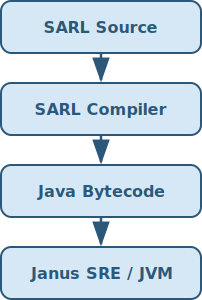
\includegraphics{sarl_pipeline}
		\end{column}
	\end{columns}
\end{frame}

\begin{frame}{{Design Principles} of SARL}
	\begin{enumerate}
	\item \Emph{Separation of Concerns} \\
	{\footnotesize What an agent \emph{can do} (Capacity) is separate from \emph{how} it does it (Skill)}
	\vspace{.3em}
	\item \Emph{Event-Driven Interaction by Default} \\
	{\footnotesize Agents communicate by default through typed, asynchronous events}
	\vspace{.3em}
	\item \Emph{Holonic / Hierarchical Organisation} \\
	{\footnotesize Agents are organized in Contexts; an agent can be a member of multiple contexts simultaneously}
	\vspace{.3em}
	\item \Emph{Openness \& Extensibility} \\
	{\footnotesize New capacities, skills and spaces can be plugged in at runtime}
	\vspace{.3em}
	\item \Emph{Platform Independence} \\
	{\footnotesize SARL code is independent of the underlying SRE; the runtime behaviour is injected via built-in capacities.}
	\end{enumerate}
\end{frame}

\figureslide{SARL Architecture}{sarl_architecture}

\begin{frame}{Holonic Architecture}
	\begin{columns}
		\begin{column}{.7\linewidth}
			SARL supports \Emph{holonic multi-agent systems}:
			\begin{itemize}
			\item Every agent \emph{defines} its own inner context
			\item Sub-agents can be spawned \emph{inside} this inner context
			\item The parent agent acts as a \Emph{super-agent} (holon)
			\item Each agent is both:
				\begin{itemize}
				\item A \emph{member} of its parent's context
				\item The \emph{super-agent} of its inner context
				\end{itemize}
			\item Enables natural hierarchical decomposition of complex systems
			\end{itemize}
		\end{column}
		\begin{column}{.3\linewidth}
			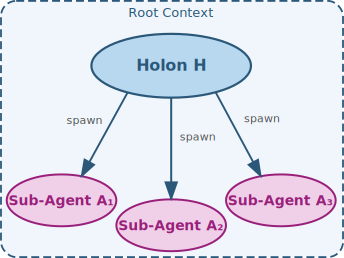
\includegraphics{sarl_holonic}
		\end{column}
	\end{columns}
\end{frame}

\begin{frame}[t]{Summary}
	\begin{block}{SARL in one sentence}
	SARL is a \Emph{general-purpose, JVM-compiled agent programming language} that provides first-class constructs for \emph{agents}, \emph{behaviors}, \emph{capacities}, \emph{skills}, \emph{events}, \emph{spaces}, and \emph{contexts} — enabling expressive, modular, and platform-independent development of multi-agent systems
	\end{block}
	\vspace{.25cm}
	\begin{columns}
		\begin{column}[t]{.5\linewidth}
			\Emph{Key strengths}
			\begin{compactitemize}
			\item Holonic architecture natively supported
			\item Clean separation of capacity and skill
			\item Reactive model via guarded behavior units
			\item Full Java interoperability
			\item Rich IDE and toolchain
			\end{compactitemize}
		\end{column}
		\begin{column}[t]{.5\linewidth}
			\Emph{Resources}
			\begin{compactitemize}
			\item Website: \texttt{http://www.sarl.io}
			\item Source:  \texttt{github.com/sarl/sarl}
			\item License: Apache 2.0
			\end{compactitemize}
		\end{column}
	\end{columns}
\end{frame}

\end{graphicspathcontext}

\endinput


	\subsection{Syntactic Basics of SARL}
	\begin{graphicspathcontext}{{./chapters/sarl/imgs/},{./chapters/sarl/imgs/auto/},\old}

\begin{frame}[t,fragile]{Java vs. SARL}
	\vspace{-.75cm}
	\begin{columns}
		\begin{column}[t]{.5\linewidth}
			\begin{javalisting}[basicstyle=\tiny]
public class ExampleOfClass
    extends SuperClass
    implements SuperInterface {
  // Field
  private int a;
  // Single-initialization field
  private final String b
                = "example";
  // Constructor
  public ExampleOfClass(int p) {
    this.a = p;
  }
  // Function with return value
  public int getA() {
    return this.a;
  }
  // Simulation of default
  // parameter value
  public void increment(int a) {
    this.a += a;
  }
  public void increment() {
    increment(1);
  }
  // Variadic parameter
  public void add(int... v) {
    for(value : v) {
      this.a += value;
    }
  }
}
\end{javalisting}
		\end{column}
		\begin{column}[t]{.5\linewidth}
			\begin{sarllisting}[basicstyle=\tiny]
class ExampleOfClass
    extends SuperClass
    implements SuperInterface {
  // Field
  var a : int
  // Single-initialization field
  // automatic detection of the
  // field type
  val b = "example"
  // Constructor
  new(p : int) {
    this.a = p
  }
  // Function with return value
  def getA : int {
    this.a
  }
  // Real default parameter value
  def increment(a : int = 1) {
    this.a += a
  }
  // Variadic parameter
  def add(v : int*) {
    for(value : v) {
      this.a += value
    }
  }
}
\end{sarllisting}
		\end{column}
	\end{columns}
\end{frame}

\begin{frame}[fragile]{Advanced Syntactic Features}
	\vspace{-.3cm}
	\begin{columns}
		\begin{column}{.15\linewidth}
			\begin{bottomarrowsequence}[width=\linewidth]
				\only<1>{\arrow[bg=CIADgreen]{\ahc{Implicit}{Get/Set}}}
				\only<2->{\arrow{\ahc{Implicit}{Get/Set}}}
				\only<2>{\arrow[bg=CIADgreen]{\ahc{Extension}{Method}}}
				\only<1,3->{\arrow{\ahc{Extension}{Method}}}
				\only<3-4>{\arrow[bg=CIADgreen]{\ahc{Lambda}{Expression}}}
				\only<1-2,5->{\arrow{\ahc{Lambda}{Expression}}}
				\only<5>{\arrow[bg=CIADgreen]{\ahc{Instance}{Variables}}}
				\only<1-4,6->{\arrow{\ahc{Instance}{Variables}}}
				\only<6->{\arrow[bg=CIADgreen]{Operators}}
				\only<1-5>{\arrow{Operators}}
			\end{bottomarrowsequence}
		\end{column}
		\begin{column}{.85\linewidth}
			\only<1>{
				\smaller
				\begin{block}{Why does it matter?}
					\Emph{Encapsulation} encourages the use of
					\texttt{getX()} / \texttt{setX()} methods instead of direct field access.
					However, calling them explicitly is \Emph{verbose} and reduces code readability \\
					\begin{example}
						\code{object.setX(object.getX + 1)}
					\end{example}
				\end{block}
				\begin{alertblock}{How does SARL resolve \texttt{variable.field}?}
					\begin{enumerate}
					\item \Emph{Read access} \textemdash{} \code{variable.field} \quad$\Rightarrow$\quad SARL first looks for \code{getField()} in the variable's type, then falls back to the accessible field \code{field}
					\item \Emph{Write access} \textemdash{} \code{variable.field = value} \quad$\Rightarrow$\quad SARL first looks for \code{setField(value)} in the variable's type, then falls back to the accessible field \code{field}.
					\end{enumerate}
					\begin{example}
						\code{object.x = object.x + 1}
					\end{example}
				\end{alertblock}
			}
			\only<2>{
				\smaller
				\begin{block}{Why does it matter?}
					Simulate the extension of existing types with new methods, \Emph{without modifying} their source code
					\begin{example}
						\code{def distance(a : String, b : String) : int \{/*Leivenstein algo*/\}} \\
						\code{distance("abc", "abz") == 1} \\
					\end{example}
				\end{block}
				\begin{alertblock}{How does SARL apply extension method?}
					\begin{itemize}
					\item \Emph{first argument} of a function can be placed \Emph{before} the function name
					\begin{example}
						\code{"abc".distance("abz") == 1} \\
					\end{example}
					\item[Note] function \Emph{distance} is unchanged. Only the \emph{call syntax} differs
					\end{itemize}
				\end{alertblock}
			}
			\only<3-4>{
				\smaller
				\begin{definitionblock}{Lambda Expression}
					Lambda expression is a \Emph{piece of code} wrapped in an object so it can be \Emph{passed around} like any other value
				\end{definitionblock}
			}
			\only<3>{
				\smaller
				\begin{compactdescription}
					\item[Syntax] \code{[ param : type, ... | code ]}
					\item[Rules] \begin{compactitemize}
						\item Parameter types may be omitted
						\item If \emph{single parameter}, it can be referred to as \code{it}
						\end{compactitemize}
						\begin{example}
							Single parameter, return the length of the parameter, use implicit name \code{it}: \\
							\code{var f = [ it.length ]}
						\end{example}
					\item[Type] Lambda expression is an object: it has a \emph{type}
						\begin{example}
							Lambda taking an \code{int} and a \code{String}, returning an \code{int}: \\
							\code{(int, String) => int}
						\end{example}
				\end{compactdescription}
      			}
			\only<4>{
				\smaller
				\begin{compactdescription}
				\item[Problem] Passing a lambda \Emph{inside} the parentheses of a call is cluttered and hard to read
				\item[Solution] If the \Emph{last parameter} of a function is a lambda expression, it can be written \Emph{outside and after} the closing parenthesis
				\end{compactdescription}
				\begin{example}
					{\code{f(a, b, [ code ])}} \quad $\Longrightarrow$ \quad {\code{f(a, b) [ code ]}}
				\end{example}
				\vspace{.25cm}
				\hiconbox{Both forms are \Emph{strictly equivalent}. The second is preferred for readability}{info-icon}
			}
			\only<5>{
				\smaller
				\begin{block}{Why does it matter?}
					Most object-oriented languages provide \Emph{special variables} that give access to key objects depending on the \Emph{current execution context}
				\end{block}
				\begin{stabularx}{l|X|X}
					\tabularhead{Variable}{Semantic}{Usage} \\
					\code{this} & Current instance of the enclosing type (class, agent, behavior...)  & Use it to access own fields and methods \\
					\hline
					\code{super} & Inherited instance, i.e., the current object seen as its parent type & Use it to call an overridden method \\
					\hline
					\code{occurrence} & Current event instance received by the agent & Available only inside an event handler \code{on EventType \{ ... \}} \\
					\hline
					\code{it} & Context-dependent object & In a lambda with a single parameter,  \code{it} is that parameter. In the expression on a event handler's guard, \code{it} is \code{occurrence}. Outside these contexts, \code{it} is unknown \\
				\end{stabularx}
      			}
      			\only<6>{
      				\smaller
      				\begin{block}{Type Operators}
		      			\begin{description}
					\item[Naming a type] Use \code{typeof(T)} to refer to a type as a value. \\
						\emph{Recommended:}\code{typeof(String)}, also valid but less explicit: \code{String}
					\item[Casting] Change the \emph{static type} of a variable at runtime: \code{variable as Type}
					\item[Type testing] Check the \Emph{actual type} of an object at runtime: \code{variable instanceof Type}
					\item[Smart cast] Inside an \code{if} block guarded by \code{instanceof}, the variable is \emph{automatically cast} -- no explicit \code{as} needed
					\end{description}
					\begin{example}
						\code{class B extends A \{ ... \}} \\
						\code{var v : A = ...} \\
						\code{if (v instanceof B) \{} \\
						\mbox{}\hspace{.25cm}\code{var v2 : B = v // No need to cast v to B} \\
						\code{\}}
					\end{example}
				\end{block}
      			}
      			\only<7>{
      				\smaller
      				\begin{block}{Equality and Comparison Operators}
					\begin{stabularx}{c|X|X}
					\tabularhead{SARL Operator}{Meaning}{Java equivalent} \\
					\code{a == b}  & Content equality & \code{a.equals(b)} \\
					\hline
					\code{a != b}  & Content inequality & \code{!a.equals(b)} \\
					\hline
					\code{a === b} & Reference equality & \code{a == b} \\
					\hline
					\code{a !== b} & Reference inequality & \code{a != b} \\
					\hline
					\code{a <=> b} & Comparison sign: $\text{sgn}(b-a) \in \{\mathbb{N}^-, 0, \mathbb{N}^+\}$ & \code{Comparable} interface \\
					\end{stabularx}
				\end{block}
				\begin{alertblock}{Key distinction: content vs.\ reference equality}
					Unlike Java, \code{==} in SARL tests \Emph{content equality} (calls \code{.equals()}), \Emph{not} reference equality. Use \code{===} for reference equality
				\end{alertblock}
      			}
      			\only<8>{
      				\smaller
      				\begin{block}{Range and Arithmetic Operators}
					\begin{stabularx}{c|X|X}
					\tabularhead{SARL Operator}{Meaning}{Java equivalent} \\
					\code{a .. b}   & Closed interval $[a,\, b]$, step $1$  & n/a \\
					\hline
					\code{a ..< b}  & Half-open interval $[a,\, b)$, step $1$ & n/a \\
					\hline
					\code{a >.. b}  & Half-open interval $(a,\, b]$, step $1$ & n/a \\
					\hline
					\code{a ** b}   & Power: $a^b$  & \code{Math.pow(a, b)} \\
					\end{stabularx}
				\end{block}
      			}
      			\only<9>{
      				\smaller
      				\begin{block}{Null-safe and Functional Operators}
					\begin{stabularx}{c|X|X}
					\tabularhead{SARL Operator}{Meaning}{Java equivalent} \\
					\code{a ?: b} & If \code{a} is not \code{null}, return \code{a}; otherwise return \code{b} & \code{a == null ? b : a} \\
					\hline
					\code{a?.b} & If \code{a} is not \code{null}, call \code{a.b}; otherwise return a default value & \code{a == null ? default : a.b} \\
					\hline
					\code{if (a) b else c} & Inline conditional expression (returns a value) & \code{a ? b : c} \\
					\hline
					\code{a -> b} & Create a \Emph{pair} $(a, b)$ & n/a \\
					\hline
					\code{a => b} & Call lambda \code{b} with \code{a} as its argument & n/a \\
					\end{stabularx}
				\end{block}
      			}
      			\only<10>{
      				\smaller
      				\begin{block}{Operator Overloading}
					Allow user-defined types to \Emph{support operators} (e.g.\ \code{+}, \code{**}) just like built-in types do
				\end{block}
				\begin{compactdescription}
				\item[Principle] Every SARL operator maps to a \Emph{reserved function name}. Defining that function in your class \textbf{overloads the operator}
				\item[Rule] \code{a OP b} $\Longrightarrow$ \code{a.operator_OPNAME(b)}
				\end{compactdescription}
				\hiconbox{If no such function is defined, a \emph{compilation error} is raised. You may also define operators on types you \emph{do not own} using \Emph{extension methods}}{info-icon}
				\begin{stabularx}{c|X}
				\tabularhead{Operator}{Function name} \\
				\code{a + b} & \code{operator\_plus(a, b)} \\
				\hline
				\code{a * b} & \code{operator\_multiply(a, b)} \\
				\hline
				\code{a ** b} & \code{operator\_power(a, b)} \\
				\hline
				\code{col += v} & \code{operator\_add(col, v)} \\
				\hline
				...
				\end{stabularx}
			}
		\end{column}
	\end{columns}
\end{frame}

\end{graphicspathcontext}

\endinput


	\subsection{Agent-Oriented Concepts}
	\subsubsection{Overview of Concepts}
	\begin{graphicspathcontext}{{./chapters/sarl/imgs/},{./chapters/sarl/imgs/auto/},\old}

\begin{frame}[c]{Overview of SARL Concepts}
	\begin{block}{Multiagent System in SARL}
	A \emph{collection of agents} interacting together in a collection of \emph{shared distributed spaces}.
	\end{block}

	\begin{scriptsize}
	\begin{columns}
		\begin{column}{0.25\linewidth}
			\begin{block}{4 main concepts}
			\begin{itemize}
			\item Agent
			\item Capacity
			\item Skill
			\item Space
			\end{itemize}
			\end{block}
		\end{column}
		\begin{column}{0.7\linewidth}
			\begin{block}{3 main dimensions}
			\begin{description}
			\item[Individual:] the Agent abstraction (Agent, Capacity, Skill)
			\item[Collective:] the Interaction abstraction (Space, Event, etc.)
			\item[Hierarchical:] the Holon abstraction (Context)
			\end{description}
			\end{block}
		\end{column}
	\end{columns}
	\begin{center}
		\textbf{SARL: {Agent-Oriented} Programming Language - Retrospective and Prospective Analysis.} Rodriguez, S., Galland, S., Gaud, N. (2026) Chapters in the book on Agents and Multi-Agent Systems Development: Platforms, Toolkits, Technologies. Chapter 2, pp. 27--54. Springer Nature, Cham, Switzerland. \cite{Rodriguez2026}	\\[.5em]
		\textbf{SARL: a general-purpose agent-oriented programming language.} Rodriguez, S., Gaud, N., Galland, S. (2014) Presented at the The 2014 IEEE/WIC/ACM International Conference on Intelligent Agent Technology, IEEE Computer Society Press, Warsaw, Poland. \cite{rodriguez_sarl:_2014} \\[1em]
		\Emph{\url{http://www.sarl.io}}
	\end{center}
	\end{scriptsize}
\end{frame}

\end{graphicspathcontext}

\endinput


	\subsubsection{Agent}
	\begin{graphicspathcontext}{{./chapters/sarl/imgs/},{./chapters/sarl/imgs/auto/},\old}

\begin{frame}{What is an Agent?}
	\begin{definitionblock}{Agent (in SARL)}
		An agent is an autonomous entity having a set of skills to realise the capacities it exhibits
	\end{definitionblock}
	\bigskip
	Three key ideas hidden in this definition:
	\begin{enumerate}
	\item \Emph{Autonomy} -- the agent decides by itself what to do and when
	\item \Emph{Capacities} -- the abstract things an agent \emph{can do}
	\item \Emph{Skills} -- the concrete implementations of those capacities
	\end{enumerate}
	\bigskip
	\begin{alertblock}{In SARL}
		An agent is a \Emph{first-class language construct}, declared with the keyword: \code{agent}
	\end{alertblock}
\end{frame}

\begin{frame}[fragile]{Declaring an Agent in SARL}
	\begin{columns}
		\begin{column}[t]{.5\linewidth}
			\Emph{Minimal agent:} \\
			\begin{sarllisting}
agent MyAgent {
	// empty: does nothing yet
}
			\end{sarllisting}
			\medskip
			\Emph{Agent with state (mental state):} \\
			\begin{sarllisting}
agent MyAgent {
	var counter : int = 0
	val name : String = "Bob"
}
			\end{sarllisting}
			\vspace{-1cm}\smaller
			\begin{itemize}
			\item \code{var} -- mutable field
			\item \code{val} -- immutable field
			\end{itemize}
		\end{column}
		\begin{column}[t]{.5\linewidth}
			\Emph{Agent with actions:} \\
			\begin{sarllisting}
import io.sarl.api.core.Logging

agent MyAgent {
	uses Logging

	def greet {
		info("Hello world!")
	}
}
			\end{sarllisting}
			\vspace{-.05cm}\smaller
			\begin{itemize}
			\item \code{def} -- defines an action
			\item \code{uses} -- imports a capacity
			\end{itemize}
		\end{column}
	\end{columns}
\end{frame}

\figureslide{{Open Architecture} of an Agent}{sarl_agent_architecture}

\begin{frame}[fragile]{Agent Life Cycle}
	Every agent follows three phases:
	\bigskip
	\begin{columns}
		\begin{column}[t]{.30\linewidth}
			\centering\textbf{\textcolor{blue!70!black}{1. Initialization}} \\[4pt]
			\begin{sarllisting}[basicstyle=\tiny]
	on Initialize {
		info("Born!")
	}
			\end{sarllisting}
		\end{column}
		\begin{column}[t]{.35\linewidth}
			\centering\textbf{\textcolor{green!50!black}{2. Lifetime}} \\[4pt]
			\begin{sarllisting}[basicstyle=\tiny]
	// Reactive
	on MyEvent {
		info("Reacting!")
	}

	// Pro-active
	on Initialize {
		every(1.seconds) [
			info("Tick")
		]
	}
			\end{sarllisting}
		\end{column}
		\begin{column}[t]{.28\linewidth}
			\centering \textbf{\textcolor{red!70!black}{3. Destruction}} \\[4pt]
			\begin{sarllisting}[basicstyle=\tiny]
uses Lifecycle

... killMe ...

on Destroy {
	info("Bye!")
}
			\end{sarllisting}
		\end{column}
	\end{columns}
	\begin{block}{Key point}
		\texttt{Initialize} and \texttt{Destroy} are \textbf{regular events}: they can be guarded, and multiple handlers can coexist (run in parallel)
	\end{block}
\end{frame}

\begin{frame}[fragile]{Agent Inheritance}
	\begin{columns}
		\begin{column}[t]{.5\linewidth}
			Agents support \Emph{single inheritance} (like Java classes):
			\begin{sarllisting}[basicstyle=\footnotesize]
agent BaseAgent {
	protected var id : int
	def logId {
		// ...
	}
}

agent SpecializedAgent
      extends BaseAgent {
	uses Logging
	on Initialize {
		id = 42
		info("I am agent #" + id)
	}
}
			\end{sarllisting}
		\end{column}
		\begin{column}[t]{.5\linewidth}
			\begin{itemize}
			\item \code{extends} -- inherits state, actions and event handlers
			\item \code{abstract agent} -- cannot be instantiated directly
			\item \code{final agent} -- cannot be further extended
			\item Specialized agent inherits from its parent: mental state, actions, behavior unit, constructors
			\item All event handlers from the parent are \emph{also executed} (in parallel with those of the child)
			\end{itemize}
		\end{column}
	\end{columns}
\end{frame}

\begin{frame}{Where Does an Agent Live?}
	\begin{columns}
		\begin{column}{.5\linewidth}
			\smaller
			\begin{itemize}
			\item When spawned, an agent joins a \code{Context}
			\item A \code{Context} gathers a set of \code{Spaces}
			\item A \code{Space} is the medium for agent interaction (default: \emph{Event Space})
			\item Every context has a \emph{Default Space} shared by all members
			\item An agent always belongs to at least one context (\emph{Default Context})
			\item An agent can join \emph{multiple external contexts}
			\item Every agent owns its own \emph{Inner Context} \\
				$\Rightarrow$ enables \emph{holonic} (nested) systems
			\end{itemize}
		\end{column}
		\begin{column}{0.5\linewidth}
			\begin{block}{Holonic Principle}
				An agent can contain other agents (sub-agents) inside its inner context, forming a \Emph{hierarchy}
			\end{block}
			\begin{example}[Universe Agent]
				At the very top of every SARL application sits the \emph{Universe Agent}, whose inner context hosts all top-level agents
			\end{example}
		\end{column}
	\end{columns}
\end{frame}

\end{graphicspathcontext}

\endinput


	\subsubsection{Capacity \& Skill}
	\begin{graphicspathcontext}{{./chapters/sarl/imgs/},{./chapters/sarl/imgs/auto/},\old}

\begin{frame}{Three Core Concepts at a Glance}
	\begin{center}
		\includegraphics[width=.72\linewidth]{sarl_capacity_skill_agent}
	\end{center}
	\vspace{.5cm}
	\begin{itemize}
	\item A \code{Capacity} defines \emph{what} an agent can do (interface)
	\item A \code{Skill} defines \emph{how} it is done (implementation)
	\item An \code{Agent} \emph{uses} capacities, fulfilled by skills at runtime
	\end{itemize}
\end{frame}

\begin{frame}[fragile]{Capacity Definition}
	\begin{block}{What is a Capacity?}
		A \code{Capacity} is the \emph{specification} of a collection of \emph{actions} (function signatures). \\
		It says \emph{what} an agent can do, \emph{not} how
	\end{block}
	\vspace{.25cm}
	\begin{itemize}
	\item Declared with the \code{capacity} keyword
	\item Contains only \emph{action signatures} -- no fields, no code bodies
	\item Compiled to a \emph{Java interface} by the SARL compiler
	\item Can extend zero or more other capacities (\code{extends})
	\end{itemize}
	\vspace{.25cm}
	\begin{sarllisting}
capacity Logging {
	// Log an information message
	def info(text : String)
	// Log a debugging message
	def debug(text : String)
}
	\end{sarllisting}
\end{frame}

\begin{frame}[fragile]{Capacity Inheritance}
	\begin{block}{Extending a Capacity}
		A capacity can \textbf{extend} one or more existing capacities, just like Java interfaces
	\end{block}
	\begin{sarllisting}
capacity ErrorLogging extends Logging {
	// Add error-level logging
	def error(text : String)
}
	\end{sarllisting}
	\begin{alertblock}{Key rule}
		A capacity can extend \Emph{zero-to-many} other capacities (multiple inheritance is allowed)
	\end{alertblock}
\end{frame}

\begin{frame}[fragile]{Skill Definition}
	\begin{block}{What is a Skill?}
		A \code{Skill} is a \emph{concrete implementation} of one or more capacities. \\
		It says \emph{how} the actions are actually performed
	\end{block}
	\vspace{.15cm}
	\begin{itemize}
	\item Declared with the \code{skill} keyword
	\item Must declare which capacity it \code{implements}
	\item Compiled to a \emph{Java class} by the SARL compiler
	\item Has a lifecycle: \code{install()} when attached, \code{uninstall()} when detached
	\end{itemize}
	\begin{sarllisting}
skill StandardLogging implements Logging {
	def info(text : String) {
		println("[INFO] " + text)
	}
	def debug(text : String) {
		println("[DEBUG] " + text)
	}
}
	\end{sarllisting}
\end{frame}

\begin{frame}[fragile]{Skill Inheritance}
	\begin{block}{Extending a Skill}
		A skill can \emph{extend} exactly \emph{one} other skill, following the same rules as Java class inheritance
	\end{block}
	\vspace{.25cm}
	\begin{sarllisting}
skill ExtendedLogging extends StandardLogging {
	def info(text : String) {
		super.info("INFO: " + text)
	}
}
	\end{sarllisting}
	\vspace{-.25cm}
	\begin{alertblock}{Key rule}
		A skill can extend \emph{at most one} other skill (single inheritance)
	\end{alertblock}
\end{frame}

\begin{frame}[t,fragile]{Giving a Skill to an Agent}
	\begin{block}{How an agent acquires a skill}
		Before using a capacity, an agent must \emph{bind} a skill to it. \\
		This is done at runtime with \code{setSkill(...)}
	\end{block}
	\begin{sarllisting}[basicstyle=\scriptsize]
agent MyAgent {
	uses Logging

	on Initialize {
		// 1. Create the skill instance
		var s = new StandardLogging
		// 2. Bind it to the capacity
		setSkill(s)
		// 3. Now we can call the capacity's actions directly
		info("Hello from MyAgent!")
	}
}
	\end{sarllisting}
	\vspace{-1cm}
	\begin{example}[Result]
		Call to \code{info(...)} is transparently dispatched to \code{StandardLogging.info(...)}
	\end{example}
\end{frame}

\begin{frame}[fragile]{Calling a Capacity via \texttt{uses}}
	\begin{columns}
		\begin{column}[t]{.5\linewidth}
			\begin{block}{Without \texttt{uses}}
				Must retrieve the skill manually:
			\end{block}
			\begin{sarllisting}
on SomeEvent {
	var s = getSkill(Logging)
	s.info("Hello")
}
			\end{sarllisting}
		\end{column}
		\begin{column}[t]{.5\linewidth}
			\begin{block}{With \texttt{uses} (recommended)}
				Capacity functions are directly available:
			\end{block}
			\begin{sarllisting}
uses Logging

on SomeEvent {
	// direct call
	info("Hello")
}
			\end{sarllisting}
		\end{column}
	\end{columns}
	\vspace{-.5cm}
	\begin{itemize}
	\item \code{uses} works as an \emph{extension method} import
	\item SARL compiler transparently routes the call to the bound skill
	\item Agent \emph{never depends on the concrete skill class} -- only on the capacity interface
	\end{itemize}
\end{frame}

\begin{frame}{Built-in Capacities}
	\begin{center}
		\Emph{SARL Agent has inherently a set of \alert{Built-in} Capacities}
	\end{center}
	\smaller
	\begin{stabularx}{l|X}
		\tabularhead{Capacity Name}{Services} \\
		\code{Behaviors} & Manage sub-behaviors \\
		\hline
		\code{Lifecycle} & Agent spawning and killing \\
		\hline
		\code{Schedules} & Scheduling of tasks \\
		\hline
		\code{ExternalContextAccess} & Access to external context \\
		\hline
		\code{InnerContextAccess} & Access to inner context \\
		\hline
		\code{DefaultContextInteractions} & Access to the default context \\
		\hline
		... & \\
	\end{stabularx}
	\hiconbox{You don't need to link the skill for those built-in capacities because the SARL runtime environment automatically equips the agent with the associated skill}{info-icon}
\end{frame}

\end{graphicspathcontext}

\endinput


	\subsubsection{Behavior}
	\begin{graphicspathcontext}{{./chapters/sarl/imgs/},{./chapters/sarl/imgs/auto/},\old}

\begin{frame}{What Is a Behavior?}
	\begin{block}{Definition}
		A \emph{behavior} maps a collection of \emph{perceptions} (represented by \emph{events}) to a sequence of \textbf{actions}
	\end{block}
	\bigskip
	\begin{itemize}
	\item A behavior is a \emph{modular piece of agent logic}
	\item It can be \emph{dynamically added or removed} from an agent at runtime
	\item It always \emph{belongs to one agent} (its \emph{owner})
	\item It shares the \emph{skills} of its owner agent
	\end{itemize}
	\bigskip
	\begin{alertblock}{Key idea}
		Instead of writing \emph{all} agent logic in one place, split it into cohesive, reusable \emph{behaviors}
	\end{alertblock}
\end{frame}

\begin{frame}[fragile]{Declaring a Behavior}
	A behavior is introduced with the \code{behavior} keyword \\[.25cm]
	\begin{columns}
		\begin{column}[t]{.5\linewidth}
			\Emph{Minimal (empty) behavior:}
			\begin{sarllisting}
behavior MyBehavior {
}
			\end{sarllisting}
			\medskip
			\Emph{With attributes (mental state):}
			\begin{sarllisting}
behavior MyBehavior {
	var counter : int = 0
	val label : String = "ok"
}
			\end{sarllisting}
		\end{column}
		\begin{column}[t]{.5\linewidth}
			\Emph{With actions (methods):}
			\begin{sarllisting}
behavior MyBehavior {
	uses Logging
	def greet {
		info("Hello!")
	}
}
			\end{sarllisting}
		\end{column}
	\end{columns}
\end{frame}

\begin{frame}[fragile]{Reactive vs.\ Pro-active Units}
	\begin{columns}
		\begin{column}[t]{.5\linewidth}
			\Emph{Reactive} — triggered by an event
			\begin{sarllisting}
behavior MyBehavior {
	uses Logging
	// optional guard in [ ]
	on SomethingChanged
	   [occurrence.value > 0] {
		info("Value changed!")
	}
}
			\end{sarllisting}
			\vspace{-.5cm}
			\begin{itemize}
			\item \code{on EventName [guard] \{ ... \}}
			\item \code{occurrence} is the received event
			\item Guard is \emph{optional}
			\item Multiple handlers run \emph{in parallel}
			\end{itemize}
		\end{column}
		\begin{column}[t]{.5\linewidth}
			\Emph{Pro-active} — self-initiated, scheduled
			\begin{sarllisting}
behavior MyBehavior {
	uses Schedules, Logging
	on Initialize {
		every(1.seconds) [
			info("I act alone!")
		]
	}
}
			\end{sarllisting}
			\vspace{-.25cm}
			\begin{itemize}
			\item The behavior \emph{schedules itself}
			\item Uses the \code{Schedules} built-in capacity
			\item No external event needed
			\end{itemize}
		\end{column}
	\end{columns}
\end{frame}

\begin{frame}[fragile]{Lifecycle of a Behavior}
	A behavior has its own \emph{lifecycle}, mirroring the agent's:
	\begin{stabularx}{lXX}
	\tabularhead{Event}{When?}{Typical use} \\
	\code{Initialize} & Behavior registered to agent & Initialise local state \\
	\hline
	Any event & While active & React / schedule tasks \\
	\hline
	\code{Destroy} & Behavior unregistered & Release resources \\
	\end{stabularx}
	\medskip
	\begin{sarllisting}
behavior MyBehavior {
	uses Logging
	on Initialize { info("Behavior started") }
	on Destroy    { info("Behavior stopped") }
}
	\end{sarllisting}
\end{frame}

\begin{frame}[fragile]{Relation Between Agent and Behavior}
	\begin{columns}
		\begin{column}{.7\linewidth}
			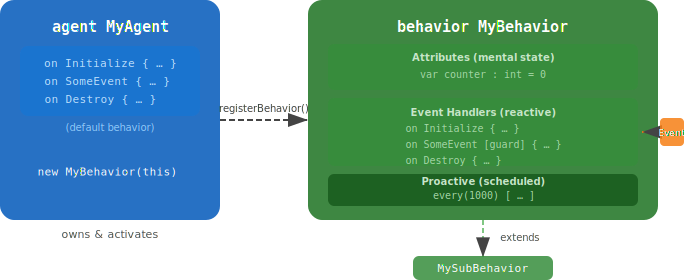
\includegraphics{sarl_behavior_agent}
		\end{column}
		\begin{column}{.3\linewidth}
			\smaller
			\Emph{How to attach a behavior to an agent:}
			\begin{sarllisting}[basicstyle=\tiny]
agent MyAgent {
	uses Behaviors

	on Initialize {
		// 1. instantiate
		var b = new MyBehavior(this)
		// 2. register
		registerBehavior(b)
	}
}
			\end{sarllisting}
			\vspace{-.5cm}
			\begin{itemize}
			\item \code{this} passes the \emph{agent as owner}
			\item \code{registerBehavior} activates event reception
			\item \code{unregisterBehavior} removes it
			\end{itemize}
		\end{column}
	\end{columns}
\end{frame}

\begin{frame}[t,fragile]{Behavior Inheritance}
	Like classes, a behavior can \emph{extend} another behavior (single inheritance):
	\begin{sarllisting}
behavior BaseBehavior {
	protected var data : String
}

behavior SpecialBehavior
         extends BaseBehavior {
	uses Logging
	on SomeEvent {
		// inherited attribute
		info("data = " + data)
	}
}
	\end{sarllisting}
	\vspace{-1cm}
	\begin{itemize}
	\item Promotes \emph{reuse} and \emph{specialisation}
	\item All \code{on Initialize} handlers from the hierarchy are run \emph{in parallel}
	\item Use \code{abstract} to create template behaviors; \code{final} to prevent further extension
	\end{itemize}
\end{frame}

\begin{frame}[fragile]{Using Capacities Inside a Behavior}
	A behavior \emph{inherits the skills} of its owner agent.
	It can also \emph{assign new skills} to the agent.
	\vspace{.25cm}
	\begin{columns}
		\begin{column}[t]{.5\linewidth}
			\Emph{Using an existing capacity:}
			\begin{sarllisting}
behavior MyBehavior {
	uses Logging, Schedules
	on SomeEvent {
		info("event received")
	}
}
			\end{sarllisting}
			\vspace{-1cm}
			\code{uses} keyword imports the capacity as an \emph{extension method}
		\end{column}
		\begin{column}[t]{.5\linewidth}
			\Emph{Assigning a skill to the agent:}
			\begin{sarllisting}
behavior MyBehavior {
	new (owner : Agent) {
		super(owner)
		setSkill(
			new MySkill(),
			typeof(MyCap))
		}
	}
			\end{sarllisting}
			\vspace{-1cm}
			Behavior can equip its agent with new capabilities at construction time
		\end{column}
	\end{columns}
\end{frame}

\end{graphicspathcontext}

\endinput


	\subsubsection{Interactions}
	\begin{graphicspathcontext}{{./chapters/sarl/imgs/},{./chapters/sarl/imgs/auto/},\old}

\begin{frame}[t]{Agents Do Not Talk Directly}
	\begin{block}{Key Principle}
		\emph{Agents never interact directly} with each other. \\
		All interactions pass through a shared \emph{interaction medium} called a \emph{Space}
	\end{block}
	\begin{columns}
		\begin{column}[t]{.5\linewidth}
			\smaller
			\Emph{Without SARL model:} \\
			\begin{itemize}
			\item Agent~A calls Agent~B directly
			\item Tight coupling
			\item Hard to control who hears what
			\end{itemize}
		\end{column}
		\begin{column}[t]{.5\linewidth}
			\smaller
			\Emph{With SARL model:} \\
			\begin{itemize}
			\item Agent~A emits an \emph{event} into a \emph{space}
			\item Agent~B is a \emph{participant} of the space and receives the event
			\item Loose coupling; fully decoupled
			\end{itemize}
		\end{column}
	\end{columns}
	\begin{center}
		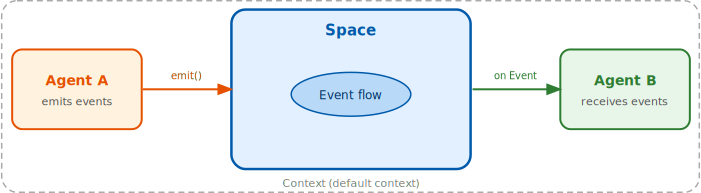
\includegraphics[width=.8\linewidth]{sarl_interactions}
	\end{center}
\end{frame}

\begin{frame}[t,fragile]{Event: The Unit of Interaction}
	\begin{block}{Definition}
		An \emph{event} is the \emph{elementary unit of interaction} inside an event space. \\
		It represents \emph{some occurrence} that may trigger a reaction in a listener
	\end{block}
	\smaller
	\begin{columns}
		\begin{column}[t]{.5\linewidth}
			\Emph{Declaring an event:}
			\begin{sarllisting}[basicstyle=\tiny]
event MyEvent {
	val message : String
	val index   : int
}
			\end{sarllisting}
			\vspace{-.5cm}
			\Emph{Key points:}
			\begin{itemize}
			\item An event carries \emph{data} (fields)
			\item Fields declared with \code{val} are read-only
			\item Events can inherit from other events
			\item Every event has a \emph{source} address (set automatically)
			\end{itemize}
		\end{column}
		\begin{column}[t]{.5\linewidth}
			\Emph{Receiving an event in an agent:}
			\begin{sarllisting}[basicstyle=\tiny]
agent MyAgent {
	uses Logging
	on MyEvent {
		// "occurrence" refers
		// to the received event
		info(occurrence.message)
	}
}
			\end{sarllisting}
			\vspace{-.5cm}
			\textbf{Emitting an event:}
			\begin{sarllisting}[basicstyle=\tiny]
agent MyAgent {
	uses DefaultContextInteractions
	def run {
		emit(new MyEvent("hi", 1))
	}
}
			\end{sarllisting}
		\end{column}
	\end{columns}
\end{frame}

\begin{frame}[fragile]{Event Hierarchy}
	\begin{block}{Events can extend other events}
		SARL events form a class hierarchy, just like Java/Xtend classes
	\end{block}
	\begin{sarllisting}[basicstyle=\scriptsize]
event BaseEvent {
	val id : int
}
event SpecialEvent extends BaseEvent {
	val extra : String
}
	\end{sarllisting}
	\vspace{-1cm}
	\begin{columns}
		\begin{column}[t]{.5\linewidth}
			\begin{description}
			\item A handler declared with \code{on BaseEvent} also fires for \code{SpecialEvent}
			\item[Built-in events] \code{Initialize}, \code{Destroy}, \code{AgentSpawned}...
			\end{description}
		\end{column}
		\begin{column}[t]{.5\linewidth}
			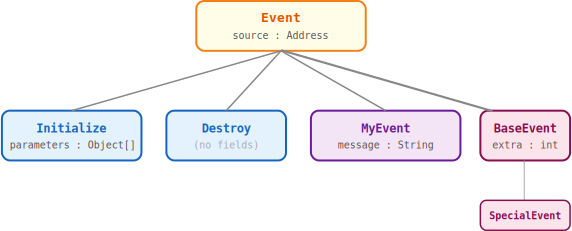
\includegraphics{sarl_event_hierarchy}
		\end{column}
	\end{columns}
\end{frame}

\begin{frame}{Space: the interaction medium}
	\begin{definitionblock}{Space}
	Space is the \emph{support} of interaction between agents, following the rules defined by its \emph{space specification}
	\end{definitionblock}
	\vspace{.5cm}
	\begin{columns}
		\begin{column}[t]{.5\linewidth}
			\Emph{Properties:}
			\begin{itemize}
			\item Identified by a unique \code{SpaceID}
			\item Contains \emph{participants} (agents)
			\item Two kinds of participant:
				\begin{description}
				\item[Strong] space is alive as long as one strong participant is present
				\item[Weak] space can be destroyed if only weak participants remain
				\end{description}
			\end{itemize}
		\end{column}
		\begin{column}[t]{.5\linewidth}
			\Emph{Key interface (simplified):}
			\begin{itemize}
			\item \code{getSpaceID()} $\to$ \code{SpaceID}
			\item \code{getNumberOfStrongParticipants()}
			\item \code{isPseudoEmpty()}
			\end{itemize}
		\end{column}
	\end{columns}
\end{frame}

\begin{frame}[t]{Event Space}
	\begin{definitionblock}{EventSpace (built-in space type)}
		SARL natively defines \code{EventSpace}, a space where agents communicate by \emph{emitting and receiving events}
	\end{definitionblock}
	\vspace{.25cm}
	\smaller
	\begin{columns}
		\begin{column}{.4\linewidth}
			\Emph{Key operations:}
			\begin{compactitemize}
			\item \code{emit(source, event)} \\
				broadcast to all
			\item \code{emit(source, event, scope)} \\
				send only to agents matching a \emph{scope}
			\item \code{getAddress(agentID)} \\
				retrieve the address of a participant
			\end{compactitemize}
			\Emph{Scope:}
			\begin{compactitemize}
			\item Predicate (filter) that selects the recipients of an event e.g., \code{Scopes.addresses(adr1, adr2)}
			\end{compactitemize}
		\end{column}
		\begin{column}{.6\linewidth}
			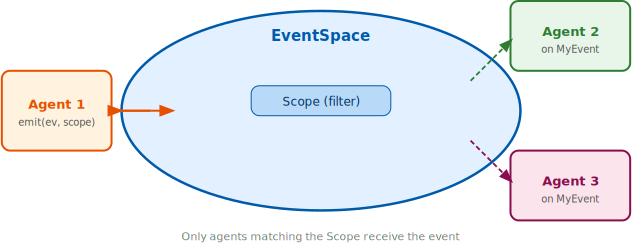
\includegraphics{sarl_event_space}
		\end{column}
	\end{columns}
\end{frame}

\begin{frame}[fragile]{{Space Specification:} Rules of a Space}
	\smaller
	\begin{definitionblock}{Space Specification}
		Defines the \emph{rules} (actions, perceptions, constraints) that govern the interaction within the spaces it creates
	\end{definitionblock}
	\begin{columns}
		\begin{column}[t]{.5\linewidth}
			\Emph{Role:}
			\begin{itemize}
			\item Acts as a \emph{factory}: creates space instances
			\item Encodes the interaction model (who can send, who can receive...)
			\item Determines the \emph{type} of space produced
			\end{itemize}
			\vspace{0.5em}
			\Emph{Built-in Specifications:}
			\begin{itemize}
			\item \code{EventSpaceSpecification} -- basic event space
			\item \code{OpenEventSpaceSpecification} -- agents freely join/leave
			\end{itemize}
		\end{column}
		\begin{column}[t]{.5\linewidth}
			\Emph{Custom specification example:}
			\begin{sarllisting}[basicstyle=\footnotesize]
class MySpaceSpec
      implements
      SpaceSpecification
               <MySpace> {
	def create(id : SpaceID,
	           params : Object*)
	    : MySpace {
		new MySpace(id)
	}
}
			\end{sarllisting}
		\end{column}
	\end{columns}
\end{frame}

\begin{frame}[fragile]{Using a Custom Space in an Agent}
	\begin{sarllisting}[basicstyle=\tiny]
agent MyAgent {
	uses DefaultContextInteractions
	uses Behaviors
	uses Logging

	var mySpace : OpenEventSpace

	on Initialize {
		// Retrieve (or create) a space matching the given spec
		mySpace = defaultContext.getOrCreateSpaceWithSpec(
				typeof(OpenEventSpaceSpecification),
				occurrence.parameters.get(0) as UUID)

		// Register this agent as a strong participant
		mySpace.registerStrongParticipant(asEventListener())
	}

	on MyEvent {
		// Handle the event received from mySpace
		info("Received: " + occurrence.message)
	}
}
\end{sarllisting}
\end{frame}

\begin{frame}{Context: A Boundary for Agent Sub-Systems}
	\begin{block}{Definition}
	A \emph{context} (AgentContext) is a \emph{container} that groups a set of spaces and defines the boundary of an agent sub-system
	\end{block}
	\vspace{.25cm}
	\begin{columns}
		\begin{column}[t]{.5\linewidth}
			\Emph{Properties:}
			\begin{itemize}
			\item Has a unique \code{UUID} identifier
			\item Contains \emph{one or more spaces}
			\item Always has a \emph{default space} (an \code{EventSpace})
			\item New spaces can be created inside a context at any time
			\item Each agent belongs to at least one context
			\end{itemize}
		\end{column}
		\begin{column}[t]{.5\linewidth}
			\Emph{Key interface (simplified):}
			\begin{itemize}
			\item \code{getID()} $\to$ \code{UUID}
			\item \code{getDefaultSpace()} $\to$ \code{EventSpace}
			\item \code{getSpaces()} $\to$ all spaces
			\item \code{createSpace(spec, id)}
			\item \code{getOrCreateSpaceWithSpec(spec, id)}
			\end{itemize}
		\end{column}
	\end{columns}
\end{frame}

\begin{frame}{{Default Context} and Default Space}
	\begin{block}{Every agent has a default context}
	When an agent is created, it is placed inside a \textbf{default context}
	with a \textbf{default space} (an \texttt{EventSpace}).\\
	The built-in capacity \texttt{DefaultContextInteractions} provides easy access to both.
	\end{block}
	\begin{center}
		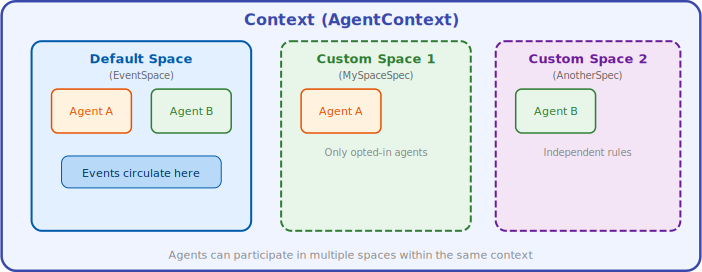
\includegraphics[width=.9\linewidth]{sarl_context_space}
	\end{center}
\end{frame}

\end{graphicspathcontext}

\endinput


	\subsubsection{Holon}
	\begin{graphicspathcontext}{{./chapters/sarl/imgs/},{./chapters/sarl/imgs/auto/},\old}

\begin{frame}{What is a Holon?}
	\begin{columns}[T]
		\begin{column}{.6\linewidth}
			\begin{block}{Origin \cite{koestler67}}
				A \emph{holon} is something that is \emph{simultaneously}:
					\begin{description}
					\item [whole] it has its own identity and autonomy
					\item [part]  it belongs to a larger whole
					\end{description}
			\end{block}
			\vspace{.5cm}
			\begin{example}
				Think of a \emph{cell} in a body:
				\begin{itemize}
				\item it lives, acts, and decides on its own
				\item yet it is a component of a tissue, an organ, an organism
				\end{itemize}
			\end{example}
			\vspace{.5cm}
		\end{column}
		\begin{column}{.4\linewidth}
			\begin{alertblock}{Key idea for SARL}
				Every SARL agent is a holon. \\
				The terms \emph{agent} and \emph{holon} are synonymous in SARL
			\end{alertblock}
			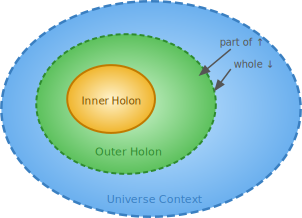
\includegraphics{sarl_holon_concept}
		\end{column}
	\end{columns}
\end{frame}

\begin{frame}[t]{Context: Shared Space between Agents}
	\begin{columns}
		\begin{column}{.5\linewidth}
			\smaller
			\begin{definitionblock}{Context}
				A \emph{context} is a shared environment in which agents live
			and interact.
				\begin{itemize}
				\item It contains one or more \emph{spaces} (interaction channels)
				\item Every context has a mandatory \emph{default space}
				\item Agents in the same context can exchange events through that default space
				\end{itemize}
			\end{definitionblock}
			\vspace{.25cm}
			\begin{block}{Two kinds of contexts for an agent}
				\begin{description}
				\item[Default context] the context in which the agent was spawned. It is its "social" environment
				\item[Inner context] the context \emph{owned} by the agent itself. Sub-agents live here
				\end{description}
			\end{block}
		\end{column}
		\begin{column}{0.5\linewidth}
			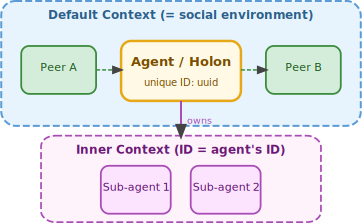
\includegraphics{sarl_agent_contexts}
		\end{column}
	\end{columns}
\end{frame}

\begin{frame}{{Inner Context:} agents inside agents}
	\smaller
	\begin{columns}
		\begin{column}{0.52\textwidth}
			\begin{block}{Every agent owns an inner context}
				\begin{itemize}
				\item An agent can \emph{spawn sub-agents} inside its own inner context
				\item The sub-agents are called \emph{sub-holons}
				\item The spawning agent becomes the \emph{super-holon} (or super-agent)
				\item The unique ID of the inner context equals the ID of its owning agent
				\end{itemize}
			\end{block}
			\hiconbox{
				An agent is \emph{always} a member of the default space of its \textbf{own inner context} \newline
				$\Rightarrow$ it can communicate with its sub-agents through that space
			}{info-icon}
		\end{column}
		\begin{column}{.5\linewidth}
			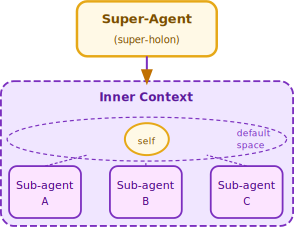
\includegraphics{sarl_inner_context}
		\end{column}
	\end{columns}
\end{frame}

\begin{frame}[t]{Holarchy: a Hierarchy of Holons}
	\smaller
	\begin{columns}
		\begin{column}{0.55\textwidth}
			\begin{definitionblock}{Holarchy \cite{koestler67}}
				A \emph{holarchy} is a recursive hierarchy of holons
				\begin{itemize}
				\item Each level is both a \emph{whole} (for the level below)
				and a \emph{part} (for the level above)
				\item The structure can be as deep as needed
				\end{itemize}
			\end{definitionblock}
			\begin{block}{At the top: the Universe Agent}
				\begin{itemize}
				\item \emph{Universe Agent} is the root of every holarchy
				\item Its inner context is the \emph{Universe Context} (called \emph{Janus Context} in the Janus runtime)
				\item All first-level agents are spawned inside it
				\end{itemize}
			\end{block}
			\begin{example}{Self-similarity}
				Each agent has the \emph{same structure}: it can always act as a simple agent \emph{and} as a container of other agents
			\end{example}
		\end{column}
		\begin{column}{.5\linewidth}
			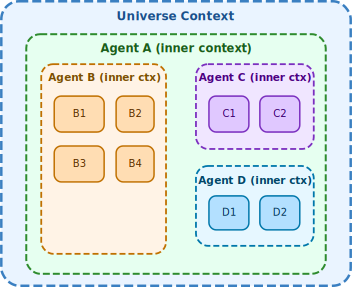
\includegraphics{sarl_holarchy}
		\end{column}
	\end{columns}
\end{frame}

\begin{frame}[fragile]{{SARL in Practice:} Super-Agent and Sub-Agent}
	\smaller
	\begin{columns}
		\begin{column}[t]{.5\linewidth}
			\Emph{Defining a sub-agent:}
			\begin{sarllisting}[basicstyle=\tiny]
agent Worker {
	uses Logging
	on PerformTask {
		// react to a task
		info("Task done!")
	}
}
			\end{sarllisting}
			\Emph{Defining the super-agent:}
			\begin{sarllisting}[basicstyle=\tiny]
agent Manager {
	uses Lifecycle
	uses InnerContextAccess

	on Initialize {
		// spawn a sub-agent
		// inside inner context
		spawnInContext(
			Worker,
			innerContext)
	}
}
			\end{sarllisting}
		\end{column}
		\begin{column}[t]{.5\linewidth}
			\Emph{Sending an event downward:}
			\begin{sarllisting}[basicstyle=\tiny]
agent Manager {
	uses Behaviors

	def requestTask {
		// wake sub-agents
		// via inner context
		wake(new PerformTask)
	}
}
			\end{sarllisting}
			\Emph{Sending an event upward:}
			\begin{sarllisting}[basicstyle=\tiny]
agent Worker {
	uses DefaultContextInteractions

	on TaskDone {
		// forward to parent
		occurrence.emitToParent
	}
}
			\end{sarllisting}
		\end{column}
	\end{columns}
\end{frame}

\end{graphicspathcontext}

\endinput


	\subsection{Official Documentation}
	\begin{graphicspathcontext}{{./chapters/sarl/imgs/},{./chapters/sarl/imgs/auto/},\old}

\begin{frame}[c]{Documentation of SARL}
	\begin{center}
		The SARL syntax is explained into the ``General Syntax Reference'' on the SARL website. \\
		\vspace{1cm}
		\url{http://www.sarl.io/docs/}
	\end{center}
\end{frame}

\end{graphicspathcontext}

\endinput


	\subsection{SARL Toolchain}
	\begin{graphicspathcontext}{{./chapters/sarl/imgs/},{./chapters/sarl/imgs/auto/},\old}

\begin{frame}[c]{Compatibility between SARL and Java}
	\alertbox{SARL is 100\% compatible with Java}
	\begin{center}
		\includegraphics[width=.9\linewidth]{sarl-compilation-process}
	\end{center}
	\begin{itemize}
	\item Any Java feature or library could be included and called from SARL.
	\item A Java application could call any public feature from the SARL API.
	\end{itemize}
\end{frame}



\begin{frame}[fragile]{Example of Convertion: Event}
	\begin{columns}[c]
		\begin{column}{.35\linewidth}
			\begin{lstlisting}
event Ping {

  var value : Integer

  new (v : int) {
    value = v
  }

}
\end{lstlisting}
		\end{column}
		\begin{column}{.05\linewidth}
			\Emph{$\Rightarrow$}
		\end{column}
		\begin{column}{.55\linewidth}
			\begin{lstlisting}[language=java]
public class Ping extends Event {

  private Integer value;

  public Ping(final int v) {
    this.value = Integer.valueOf(v);
  }

}
\end{lstlisting}
		\end{column}
	\end{columns}
\end{frame}



\begin{frame}[fragile]{Example of Convertion: Agent}
	\begin{columns}[c]
		\begin{column}{.45\linewidth}
			\begin{lstlisting}
agent PongAgent {
  uses
    DefaultContextInteractions

  on Initialize {
    println(
      "Waiting for ping")
  }

  on Ping {
    println(
       "Recv Ping: " +
       occurrence.value)
    println(
       "Send Pong: " +
       occurrence.value)
    emit(new Pong(
      occurrence.value))
  }
}
\end{lstlisting}
		\end{column}
		\begin{column}{.05\linewidth}
			\Emph{$\Rightarrow$}
		\end{column}
		\begin{column}{.55\linewidth}
			\begin{lstlisting}[language=java]
public class PongAgent extends Agent {

  public PongAgent(final UUID parent,
           final UUID id) {
    super(parent, id);
  }


  @PerceptGuardEvaluator
  private void $guard$Initialize(
      final Initialize occurrence,
      final Collection<Runnable>
        $handlers) {
    final Ping it = occurrence;
    $handlers.add( () ->
      $on$Initialize(occurrence));
  }

  private void $on$Initialize(
      final Initialize occurrence) {
    System.out.println(
      "Waiting for ping");
  }
\end{lstlisting}
		\end{column}
	\end{columns}
\end{frame}


\begin{frame}[fragile]{Example of Convertion: Agent}
	\begin{columns}[c]
		\begin{column}{.45\linewidth}
			\begin{lstlisting}
agent PongAgent {
  uses
    DefaultContextInteractions

  on Initialize {
    println(
      "Waiting for ping")
  }

  on Ping {
    println(
       "Recv Ping: " +
       occurrence.value)
    println(
       "Send Pong: " +
       occurrence.value)
    emit(new Pong(
      occurrence.value))
  }
}
\end{lstlisting}
		\end{column}
		\begin{column}{.05\linewidth}
			\Emph{$\Rightarrow$}
		\end{column}
		\begin{column}{.55\linewidth}
			\begin{lstlisting}[language=java]
  @PerceptGuardEvaluator
  private void $guard$Ping(
      final Ping occurrence,
      final Collection<Runnable>
        $handlers) {
    final Ping it = occurrence;
    $handlers.add( () ->
      $on$Ping(occurrence));
  }

  private void $on$Ping(
      final Ping occurrence) {
    System.out.println("Recv Ping: "
      + occurrence.value);
    System.out.println("Send Pong: "
      + occurrence.value);
    final DefaultContextInteractions s
      = getSkill(
    DefaultContextInteractions.class);
    s.emit(new Pong(
      occurrence.value));
  }

}
\end{lstlisting}
		\end{column}
	\end{columns}
\end{frame}

\figureslide{SARL in the Eclipse IDE}{eclipse_about}

\begin{frame}[t]{Runtime Environment for SARL (SRE)}
	\smaller
	\begin{block}{Runtime Environment Requirements}	
	\begin{itemize}
		\item Implements SARL concepts.
		\item Provides Built-in Capacities.
		\item Handles Agent's Lifecycle.
		\item Handles resources.
	\end{itemize}
	\end{block}
	\begin{block}{Janus as a SARL Runtime Environment}
		\wrapfigure[width=1.5cm]{janus}
		\begin{itemize}
		\wrapitem{\alert{Fully distributed}.}
		\wrapitem{\alert{Dynamic discovery of Kernels}.}
		\wrapitem{\alert{Automatic synchronization of kernels' data (easy recovery)}.}
		\item Micro-Kernel implementation.
		\item Official website: \url{https://www.sarl.io/runtime/janus/}
		\end{itemize}
	\end{block}
\end{frame}

\end{graphicspathcontext}

\endinput



\end{bibliographysection}

\part{Multiagent-based Simulation}
\begin{bibliographysection}

	\section[Simulation Basics]{Basics of Simulation}
	\begin{graphicspathcontext}{{./chapters/simulation/imgs/},{./chapters/simulation/imgs/auto/},\old}

\begin{frame}{{Several Definitions} of Simulation}
	\begin{definitionblock}{\cite{Shannon77}}
		The process of \Emph{designing a model} of a real system and \Emph{conducting experiments } with this model for the purpose either of \Emph{understanding} the behavior of the system or of \Emph{evaluating} various strategies (within the limits imposed by a criterion or a set of criteria) for the operation of the system.
	\end{definitionblock}
	\vspace{.5cm}
	\begin{definitionblock}{\cite{Fishwick97}}
		Computer simulation is the discipline of designing a model of an actual or theoritical physical system, executing the model on a digital computer, and analyzing the execution output.
	\end{definitionblock}
\end{frame}

\sidenote{Image Claude Sonnet 4.6}
\figureslide{{Standard Lifecycle} of a Simulation Model}{simulation_lifecycle}

\sidecite{Zeigler00}
\figureslide{Relation between the real system and the simulation model}{simulation_basics}

\sidecite{Zeigler00}
\begin{frame}[t]{{Modeling Relation:} System $\leftrightarrow$ Model}
	\begin{center}
		\includegraphics[width=.8\linewidth]{system_model_relation}
	\end{center}
	\vspace{.5cm}
	\begin{itemize}
	\item To determine if the system model is an acceptable simplificiation in terms of quality criteria and experimentation objectives.
	\item Directly related to the consistency of the model simulation.
	\end{itemize}
\end{frame}

\sidecite{Zeigler00}
\begin{frame}[t]{{Simulation Relation:} Model $\leftrightarrow$ Simulator}
	\begin{center}
		\includegraphics[width=.8\linewidth]{model_simulator_relation}
	\end{center}
	\vspace{.5cm}
	\begin{itemize}
	\item To guarantee that the simulator, used to implement the model, correctly generates the behavior of the model.
	\item To be sure that the simulator reproduces clearly the mechanisms of change of state are formalized in the model.
	\end{itemize}
\end{frame}

\sidenote{Images Claude Sonnet 4.6}
\begin{frame}[t]{What is simulated?}
	\begin{columns}
		\begin{column}[t]{.5\linewidth}
			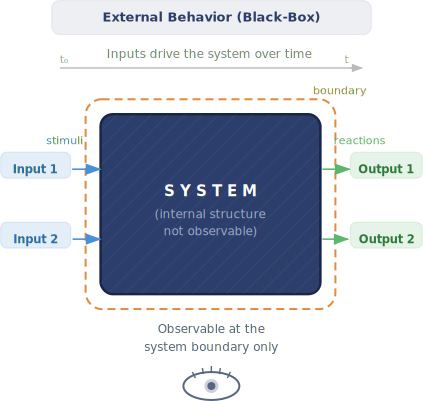
\includegraphics{simulation_external_behavior}
		\end{column}
		\begin{column}[t]{.5\linewidth}
			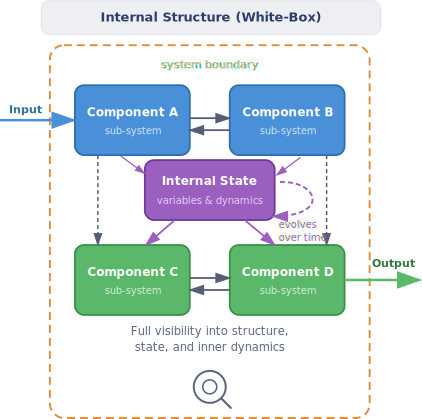
\includegraphics{simulation_internal_structure}
		\end{column}
	\end{columns}
\end{frame}

\begin{frame}[t]{{System Dynamic:} Defining the Time Advance Function}
	\vspace{-.5cm}
	\begin{columns}
		\begin{column}[t]{.2\linewidth}
			\begin{bottomarrowsequence}
				\only<1>{\arrow[bg=CIADgreen]{Continuous Time}}
				\only<2->{\arrow{Continuous Time}}
				\only<1,3>{\arrow{Discrete Time}}
				\only<2>{\arrow[bg=CIADgreen]{Discrete Time}}
				\only<1-2>{\arrow{\ahc{Event-based}{Time}}}
				\only<3>{\arrow[bg=CIADgreen]{\ahc{Event-based}{Time}}}
			\end{bottomarrowsequence}
		\end{column}
		\begin{column}[t]{.8\linewidth}
			\only<1>{
				\smaller
				\begin{block}{Principle}
					\begin{compactitemize}
						\item Time $t \in \mathbb{R}_{\geq 0}$ flows \emph{continuously} and without interruption
						\item The system state $\mathbf{x}(t)$ is defined at \emph{every} instant $t$
						\item The dynamics are governed by a system of \Emph{ordinary differential equations}
					\end{compactitemize}
				\end{block}
				\begin{block}{Mathematical Model}
					\begin{compactdescription}
					\item[State Evolution] $\frac{d\,\mathbf{x}(t)}{dt} = f\!\bigl(\mathbf{x}(t),\,\mathbf{u}(t),\,t\bigr), \quad \mathbf{x}(t_0) = \mathbf{x}_0$
					\item[Output] $\mathbf{y}(t) = g\!\bigl(\mathbf{x}(t),\,\mathbf{u}(t),\,t\bigr)$
					\end{compactdescription}
					where $\mathbf{x}\!\in\!\mathbb{R}^n$ is the state vector, $\mathbf{u}\!\in\!\mathbb{R}^m$ the input, and $\mathbf{y}\!\in\!\mathbb{R}^p$ the output
				\end{block}
				\centering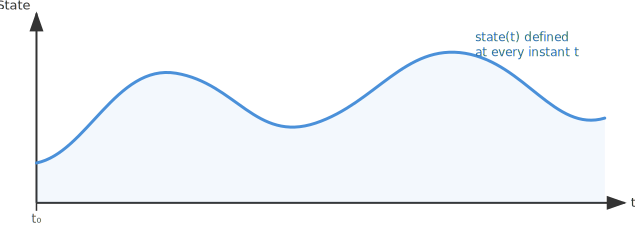
\includegraphics[width=.8\linewidth]{time_continuous}
			}
			\only<2>{
				\smaller
				\begin{block}{Principle}
					\begin{compactitemize}
						\item Time advances in \emph{uniform steps}: $t_k = t_0 + k\,\Delta t, \quad k \in \mathbb{N}$
						\item The system state $\mathbf{x}_k$ is only defined \emph{at the discrete instants} $t_k$
						\item Between two steps, the state is \Emph{not observed}
					\end{compactitemize}
				\end{block}
				\begin{block}{Mathematical Model}
					\begin{compactdescription}
					\item[State Evolution] $\mathbf{x}_{k+1} = f\!\bigl(\mathbf{x}_k,\,\mathbf{u}_k,\,k\bigr), \quad \mathbf{x}_0 \text{ given}$
					\item[Output] $\mathbf{y}_k = g\!\bigl(\mathbf{x}_k,\,\mathbf{u}_k,\,k\bigr)$
					\end{compactdescription}
					where $\mathbf{x}\!\in\!\mathbb{R}^n$ is the state vector, $\mathbf{u}\!\in\!\mathbb{R}^m$ the input, and $\mathbf{y}\!\in\!\mathbb{R}^p$ the output
				\end{block}
				\centering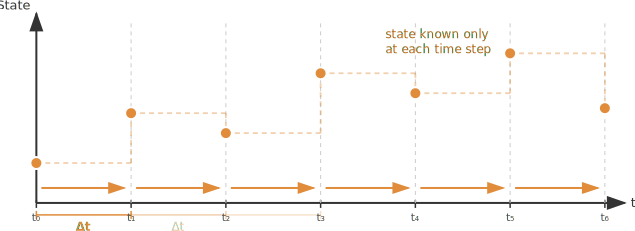
\includegraphics[width=.8\linewidth]{time_discrete_constant}
			}
			\only<3>{
				\smaller
				\begin{block}{Principle}
					\begin{compactitemize}
						\item Time advances \emph{only when an event occurs}
						\item Between two consecutive events, the state is \Emph{constant}
						\item Time steps $\Delta t_k$ are \Emph{variable} and determined by the event schedule
					\end{compactitemize}
				\end{block}
				\begin{block}{Mathematical Model}
					Let $\mathcal{E} = \{e_1, e_2, \ldots\}$ the ordered sequence of events
					\begin{compactdescription}
					\item[Time Advance Evolution] $\Delta t_k = t_{k+1} - t_k > 0$
					\item[State transition at event $e_k$] $\mathbf{x}(t_k+1) = \delta\!\bigl(\mathbf{x}(t_k),\, e_k\bigr)$
					\end{compactdescription}
				\end{block}
				\centering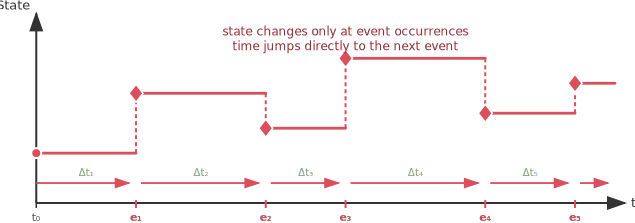
\includegraphics[width=.8\linewidth]{time_event_based}
      			}
		\end{column}
	\end{columns}
\end{frame}

\sidenote{\cite{Hoogendoorn01, Davidsson00}, Image Claude Sonnet 4.6}
\figureslide{{Standard Scales} of Simulation Models}{simulation_model_scales}

\begin{frame}{{Macroscopic Model:} Advantages and Disadvantages}
	\hiconbox{
		\begin{compactdescription}
		\item[Low computational cost] few variables, fast execution
		\item[Scalable] to very large systems without additional cost
		\item[Analytically tractable] closed-form solutions often exist
		\item[Simple to calibrate] aggregate data usually available
		\item[Stable] numerical behaviour with well-known solvers
		\end{compactdescription}}{simu-pros-icon}
	\hiconbox{
		\begin{compactdescription}
		\item[Low accuracy] at fine scales individual behaviour is lost
		\item[Cannot capture] local interactions, heterogeneity, or emergent phenomena
		\item[Strong assumptions] required (homogeneity, mean-field, \ldots)
		\item[Poor predictive power] when individual variability matters
		\item[Validation is difficult] when no aggregate ground truth exists
		\end{compactdescription}}{simu-cons-icon}
\end{frame}

\begin{frame}{{Mesoscopic Model:} Advantages and Disadvantages}
	\hiconbox{
		\begin{compactdescription}
		\item[Balanced trade-off] between accuracy and computational cost
		\item[Captures group dynamics] and statistical heterogeneity
		\item[More realistic] than macro without the cost of micro
		\item[Flexible granularity] group size can be tuned
		\item[Compatible] with both macro and micro representations, enabling multilevel coupling
		\end{compactdescription}}{simu-pros-icon}
	\hiconbox{
		\begin{compactdescription}
		\item[More complex] to design and implement than macro models
		\item[Higher cost] than macro, lower accuracy than micro
		\item[Requires statistical data] for calibrating distributions
		\item[Group boundaries] may be arbitrary and hard to justify
		\item[Emergent individual behaviour] not fully captured
		\end{compactdescription}}{simu-cons-icon}
\end{frame}

\begin{frame}{{Microscopic Model:} Advantages and Disadvantages}
	\hiconbox{
		\begin{compactdescription}
		\item[Highest accuracy] individual behaviour fully represented
		\item[Captures emergent phenomena] arising from local interactions
		\item[Heterogeneity] modelled naturally per entity
		\item[No aggregation assumptions] results are more faithful to reality
		\item[Rich observable outputs] individual trajectories available
		\end{compactdescription}}{simu-pros-icon}
	\hiconbox{
		\begin{compactdescription}
		\item[Very high computational cost] scales poorly with system size
		\item[Large memory footprint] one state record per entity
		\item[Hard to calibrate] individual-level data rarely available
		\item[Complex to implement] and to verify
		\item[Results hard to interpret] at the global scale without post-processing aggregation
		\end{compactdescription}}{simu-cons-icon}
\end{frame}

\sidenote{\cite{GallandGaudDemangeKoukam2014_703}, Images Claude Sonnet 4.6}
\begin{frame}[t]{{Multilevel Model:} coupled models or dynamic model}
	\begin{columns}
		\begin{column}{.5\linewidth}
			\centering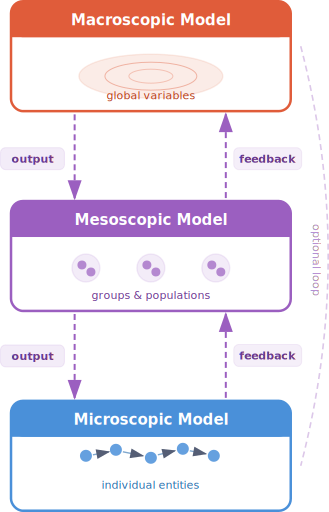
\includegraphics[height=.9\textheight]{multilevel_coupling}
		\end{column}
		\begin{column}{.5\linewidth}
			\centering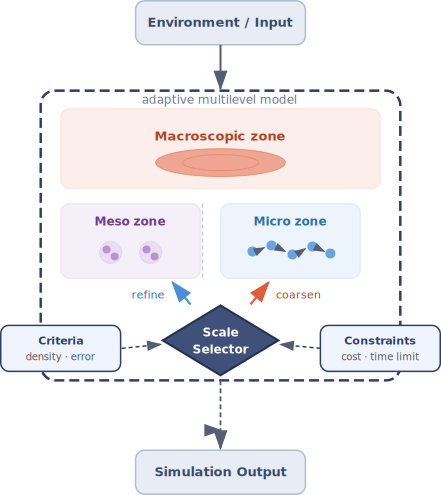
\includegraphics[height=.9\textheight]{multilevel_dynamic}
		\end{column}
	\end{columns}
\end{frame}

\end{graphicspathcontext}

\endinput



	\section[MABS Principles]{Principles of Multiagent-based Simulation}
	\begin{graphicspathcontext}{{./chapters/simulation/imgs/},{./chapters/simulation/imgs/auto/},\old}

\begin{frame}{What is Multiagent-based Simulation?}
	\begin{definition}
		Multiagent-based Simulation (MABS) is a computational methodology that models a system as a collection of \Emph{autonomous, interacting agents} situated in an explicit \Emph{environment}, whose \Emph{local interactions} give rise to \Emph{global, emergent phenomena}.
	\end{definition}
	\vspace{.5cm}
	\begin{itemize}
	\item Rooted in \Emph{Complex Systems} science
	\item Bridges \Emph{Agent-Oriented Programming} and \Emph{Simulation Science}
	\item Particularly suited to \emph{heterogeneous}, \emph{decentralised}, and \emph{adaptive} systems
	\end{itemize}
\end{frame}

\begin{frame}[t]{Core Concepts}
	\vspace{-.5cm}
	\begin{columns}
		\begin{column}[t]{.5\linewidth}
			\smaller
			\begin{block}{Agent}
				An \emph{autonomous entity} that:
				\begin{description}
				\item[Perceives] its environment via sensors
				\item[Decides] according to its internal state \& goals
				\item[Acts] to modify itself or the environment
				\item May \Emph{communicate} with other agents
				\end{description}
			\end{block}
			\begin{block}{Interaction}
				Agents interact \Emph{locally}:
				\begin{itemize}
				\item Direct communication
				\item Indirect through environment (stigmergy)
				\item coordination, cooperation, negotiation, competition
				\end{itemize}
			\end{block}
		\end{column}
		\begin{column}[t]{.5\linewidth}
			\smaller
			\begin{block}{Agent Environment}
				\Emph{Shared medium} in which agents are situated:
				\begin{itemize}
				\item Carries \emph{spatial} and \emph{temporal} structure
				\item Mediates \emph{indirect interaction} (stigmergy)
				\item Can itself be \emph{dynamic} or \emph{reactive}
				\end{itemize}
			\end{block}
			\begin{block}{Emergence}
				\Emph{Global patterns} arise from local rules:
				\begin{itemize}
				\item Not explicitly programmed
				\item Cannot be predicted from individual behaviour alone
				\end{itemize}
			\end{block}
		\end{column}
	\end{columns}
\end{frame}

\begin{frame}{Advantages of Multiagent-based Simulation}
	\hiconbox{
		\begin{compactdescription}
		\item[Individual heterogeneity] each agent has its own
		state, rules, and objectives
		\item[Spatial explicitness] agents are situated in a topology; local interactions are first-class citizens
		\item[Emergence] complex global patterns arise \emph{bottom-up} from local rules, without explicit global equations
		\item[Adaptive behaviour] agents learn and change strategy over time
		\item[Stochasticity at the micro level] individual variability and rare events are handled naturally
  		\end{compactdescription}}{simu-pros-icon}
\end{frame}

\begin{frame}{Disadvantages of Multiagent-based Simulation}
	\hiconbox{
		\begin{compactdescription}
		\item[No analytical tractability] unlike EBM/SD, closed-form solutions or stability analyses are rarely possible
		\item[Difficult validation] emergent behaviour is hard to verify against real data; risk of over-fitting micro rules
		\item[Parameter explosion] many agent-level parameters must be estimated, calibrated, and sensitivity-tested
		\item[Non-determinism] stochastic runs require statistical analysis of many replications
		\item[Computational cost] large populations of agents are expensive; scaling is non-trivial
		\item[Development complexity] building, debugging, and maintaining agent code is more demanding than scripting equations
		\end{compactdescription}}{simu-cons-icon}
\end{frame}

\end{graphicspathcontext}

\endinput


	\section[MABS Simulator]{Multiagent-based Simulator}
	\subsection{Simulation Architecture}
	\begin{graphicspathcontext}{{./chapters/simulation/imgs/},{./chapters/simulation/imgs/auto/},\old}

\figureslide{Overview of a MABS Architecture}{mabs_overview}

\sidecite{Michel04}
\figureslide{Designing a Multiagent Simulation Model}{model_design}

\sidecite{Michon85,Hoogendoorn01,Hoogendoorn04}
\begin{frame}{Three-Layer Architecture}
	\begin{columns}
		\begin{column}[c]{.6\linewidth}
			\begin{description}
			\item[Strategic Layer] general planning stage that includes the determination of goals, the route and
the modal choice as well as a cost-risk evaluation.
			\item[Tactic Layer] Maneuvering level behavior. Examples: obstacle avoidance, gap acceptance, turning, and overtaking.
			\item[Operational Layer] Fundamental body controlling processes such as controlling speed, following the path, etc.
			\end{description}
		\end{column}
		\begin{column}[c]{.4\linewidth}
			\raisebox{-\height}{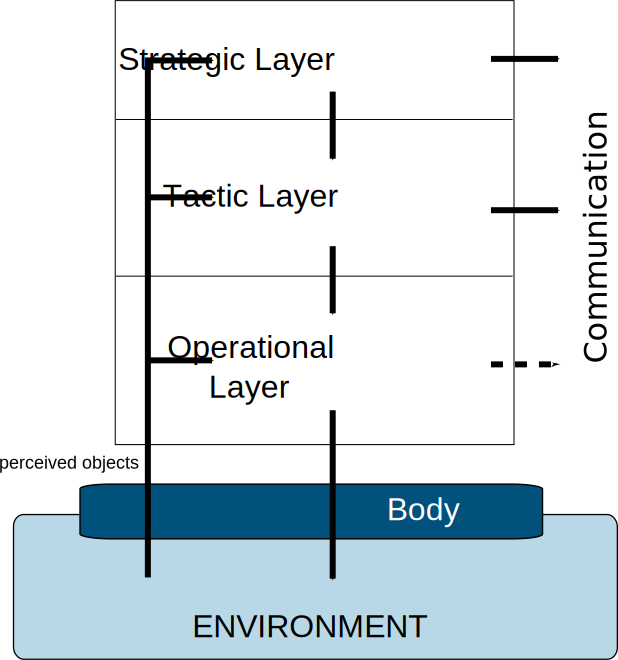
\includegraphics{standard_agent_layers}}
		\end{column}
	\end{columns}
\end{frame}

\sidecite{brooks90}
\begin{frame}[t,fragile]{{Operational Layer Example:} Subsumption Architecture}
	\begin{itemize}
	\item Priority-ordering sequence of condition-action pairs.
	\item Mostly contributes to the lower level in the three-layer architecture. 
	\end{itemize}
	\vspace{.25cm}
	\begin{columns}[t]
		\begin{column}{.39\linewidth}
			\begin{lstlisting}[basicstyle=\scriptsize]
if condition1
   action1
else if condition2
   action2
else
   ...
			\end{lstlisting}
		\end{column}
		\begin{column}{.59\linewidth}
			\raisebox{-\height}{\includegraphicswtex[width=\linewidth]{subsomption}}
		\end{column}
	\end{columns}
\end{frame}

\sidecite{Helbing.1997,Reynolds.99,buisson.abmtrans13}
\begin{frame}[t]{{Tactic Layer Example:} (Social) Force Models}
	\begin{itemize}
	\item Repulsive forces are computed and summed for obtaining the safer direction.
	\item Mostly contributes to the two lower layers of the three-layer architecture. 
	\end{itemize}
	\begin{columns}
		\begin{column}{.7\linewidth}
			\centering
			{\smaller\smaller$\vec{f} = \vec{f}_1 + \vec{f}_2 + \epsilon_1 =
				\left( \sum^k_{i=1} \dfrac{\alpha_i.\widehat{c-a_i}}{|\overrightarrow{c-a_i}|} \right)
				+ \left( \dfrac{\beta.\overrightarrow{\dfrac{\sum^k_{i=1} a_i}{k} - c}}{\left|\overrightarrow{\dfrac{\sum^k_{i=1} a_i}{k} - c}\right|^2} \right)
				+ \epsilon_1
			$}
		\end{column}
		\begin{column}{.2\linewidth}
			\centering
			{\smaller\smaller$\theta =
				\dfrac{\sum^k_{i=1} \theta_i}{k}
				+ \epsilon_2
			$}
		\end{column}
	\end{columns}
	where: $c$ is the current agent, $(a_1,\cdots,a_k)$ are the perceived agents, $\theta_i$ is the orientation of $a_i$
	\begin{center}
			\begin{tabular}{c@{\hspace{2em}}c@{\hspace{2em}}c@{\hspace{2em}}c@{\hspace{2em}}c}
				\includegraphicswtex[width=.15\linewidth]{boids_separation} &
				{\Huge $+$} &
				\includegraphicswtex[width=.15\linewidth]{boids_cohesion} &
				{\Huge $+$} &
				\includegraphicswtex[width=.15\linewidth]{boids_alignment} \\
				\small separation $\vec{f}_1$ & &
				\small cohesion $\vec{f}_2$ & &
				\small alignment $\theta$ \\
			\end{tabular}
	\end{center}
\end{frame}

\sidenote{\cite{Rao95}, Image Claude Sonnet 4.6}
\figureslide{{Stategic Layer Example:} Belief, Desire, Intention (BDI) Architecture}{bdi_rao_lifecycle}

\sidecite{Harel.87.statechart,Baum66,Rumbaugh99}
\begin{frame}[t,fragile]{{Multilayer Example:} State-Transition Diagrams}
	\begin{itemize}
	\item Define the behavior in terms of states and transitions
	\item Actions may be trigerred on transitions or states
	\item Markov models \cite{Baum66} or activity diagrams \cite{Rumbaugh99} may be used in place of state-transition diagrams
	\end{itemize}
	\begin{columns}
		\begin{column}[t]{.4\linewidth}
			\begin{sarllisting}[basicstyle=\tiny]
agent VaacumRobot {

  var state = Iddle

  on Perception
     [state == Navigating &&
      occurrence.contains(Durty)] {
    state = Cleaning
    suck()
  }

  on Perception
     [state == Cleaning &&
      occurrence.contains(DurtyBinFull)] {
    state = ReturningToDock
    moveToDock()
  }
  ...
}
			\end{sarllisting}
		\end{column}
		\begin{column}[t]{.4\linewidth}
			\raisebox{-\height}{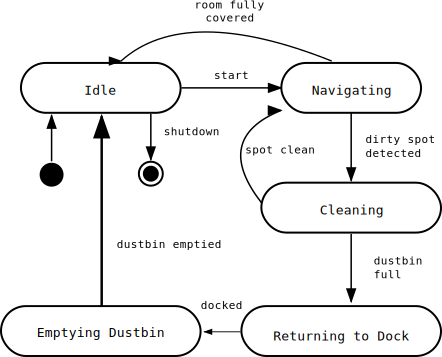
\includegraphics{vacuum_robot_state_diagram}}
		\end{column}
	\end{columns}
\end{frame}

\end{graphicspathcontext}

\endinput


	\subsection{Agent Environment}
	\begin{graphicspathcontext}{{./chapters/simulation/imgs/},{./chapters/simulation/imgs/auto/},{./chapters/mas/imgs/auto/}\old}

\begin{frame}{What is the Agent Environment?} 
	\begin{definitionblock}{Agent Environment \cite{weyns2007environment}}
		The environment is a first-class abstraction that provides the agents with a computational infrastructure and a set of services to facilitate agent interaction and situatedness.
	\end{definitionblock}
	
	\begin{block}{Properties}
		\begin{description}
		\item[Situatedness] Agents are situated in the environment; they perceive it through sensors and act upon it through actuators
		\item[Medium for interaction] The environment mediates all interactions among agents (indirect, e.g., stigmergy)
		\item[Active role] The environment is not merely a passive container; it has its own dynamics, laws, and computational processes independent of agents
		\item[Services provider] The environment offers services to agents (e.g., communication, coordination, spatial reasoning)
		\end{description}
	\end{block}
\end{frame}

\begin{frame}{{Formal Definition} of the Agent Environment} 
	\[E = \langle O, Ag, R, L, \Omega, \tau \rangle\]
	\begin{stabularx}{l|X}
		\tabularhead{Symbol}{Description} \\
		$O$ & Set of objects (passive entities) in the environment \\
		$Ag$ & Set of agents situated in the environment \\
		$R$ & Set of relations among objects and agents \\
		$L$ & Set of laws governing the environment's dynamics \\
		$\Omega$ & Set of observable properties of the environment \\
		$\tau$ & The time model governing state transitions \\
	\end{stabularx}
\end{frame}

\sidenote{Mix of the archectures given by \cite{weyns2007environment,Weyns05,Viroli07}}
%\animatedfigureslide[width=.75\linewidth]{Environment Layers}{environment_layers} 
\figureslide{Environment Layers}{environment_layers_full} 

\begin{frame}{{Key Properties} of the Agent Environment}
	\vspace{-.25cm}
	\begin{columns}
		\begin{column}{.2\linewidth}
			\begin{bottomarrowsequence}
				\only<1>{\arrow[bg=CIADgreen]{Observability}}
				\only<2->{\arrow{Observability}}
				\only<2>{\arrow[bg=CIADgreen]{Determinism}}
				\only<1,3->{\arrow{Determinism}}
				\only<3>{\arrow[bg=CIADgreen]{Dimensionality}}
				\only<1-2,4>{\arrow{Dimensionality}}
				\only<4>{\arrow[bg=CIADgreen]{Dynamicity}}
				\only<1-3>{\arrow{Dynamicity}}
			\end{bottomarrowsequence}
		\end{column}
		\begin{column}{.8\linewidth}
			\only<1>{
				\smaller
				\begin{block}{Fully Observable Environment}
					\begin{itemize}
					\item \Emph{All aspects} of the environment are visible
					\item \Emph{Complete, accurate, and up-to-date} knowledge of the environment state
					\end{itemize}
				\end{block}
				\begin{block}{Partially Observable Environment}
					\begin{itemize}
					\item Observability is limited in space and time and specific to each agent
					\item Agent maintains \Emph{internal model} to track sensed information
					\item \Emph{Other agents' intentions} are not observable, even if their actions are
					\end{itemize}
				\end{block}
				\centering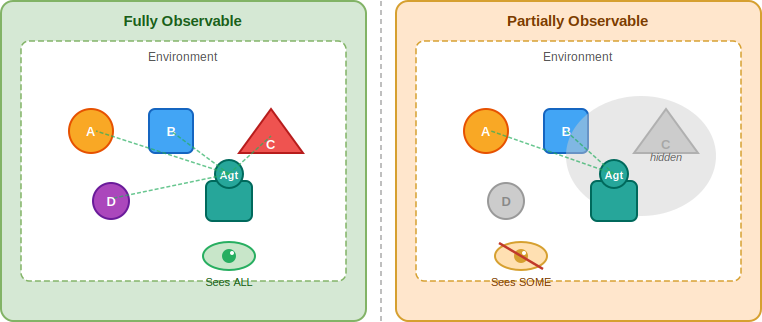
\includegraphics[width=.6\linewidth]{environment_observability}
			}
			\only<2>{
				\smaller
				\begin{columns}
					\begin{column}{.5\linewidth}
						\begin{block}{Deterministic Environment}
							\Emph{Next state} of the environment is \Emph{completely predictable} from the current state and the action executed by the agent
						\end{block}
					\end{column}
					\begin{column}{.5\linewidth}
						\begin{block}{Stochastic Environment}
							\Emph{Next state} has \Emph{some uncertainty} due to randomness, incomplete or inaccurate models, incomplete sensor coverage
						\end{block}
					\end{column}
				\end{columns}
				\vspace{-.2cm}
				\begin{alertblock}{Strategic Environment}
					\begin{itemize}
					\item Environment that is \Emph{deterministic except for the actions from agents}
					\item Agents introduce \Emph{apparent} stochasticity from the perspective of a single agent, even if the underlying physics are deterministic
					\end{itemize}
				\end{alertblock}
				\centering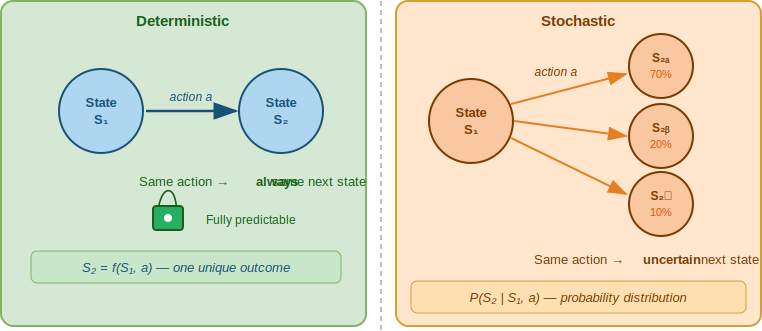
\includegraphics[width=.62\linewidth]{environment_determinism}
  			}
  			\only<3>{
				\smaller
				\begin{block}{Discrete Environment}
					\begin{itemize}
					\item \Emph{State space} and \Emph{action space} are finite or countably infinite
					\item Coordinates space is discrete and usually based on \Emph{integer values}
					\end{itemize}
				\end{block}
				\begin{block}{Continuous Environment}
					\begin{itemize}
					\item \Emph{State space} and \Emph{action space} are real-valued and potentially infinite-dimensional
					\item Coordinates space is continuous and usually based on \Emph{floating-point number values}
					\end{itemize}
				\end{block}
				\centering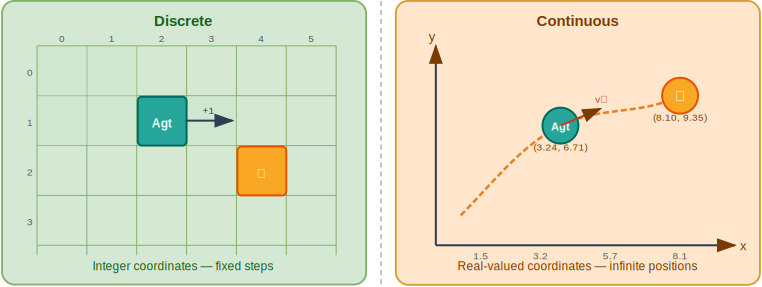
\includegraphics[width=.7\linewidth]{environment_dimensionality}
  			}
			\only<4>{
				\smaller
				\begin{block}{Dynamic Environment}
					\begin{itemize}
					\item Environment \Emph{may change over time}, independently of the agent's own actions
					\item Definition of endogenous dynamics engine
					\end{itemize}
				\end{block}
				\begin{block}{Static Environment}
					\begin{itemize}
					\item \Emph{Nothing changes} in the environment except as a direct result of the agent's own actions
					\end{itemize}
				\end{block}
				\centering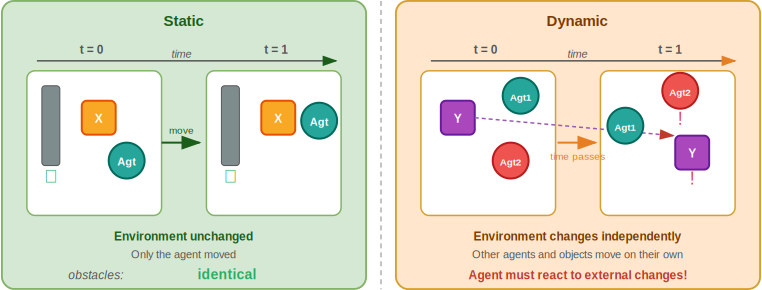
\includegraphics[width=.8\linewidth]{environment_dynamicity}
  			}
		\end{column}
	\end{columns}
\end{frame}

\sidecite{Weyns05}
\begin{frame}{Missions of the Environment}
	\begin{description}
	\item<1->[M1 - Sharing informations] Environment is a shared structure for agents, where each of them perceives and acts.
	\item<2->[M2 - Managing perception and observation] Agents can manage the access to environmental informations and guarantee the partialness and localness of perceptions.
	\item<3->[M3 - Managing agents actions and interactions] It is related to the management of agents' simultaneous and joint actions and to the preservation of the environmental integrity: influence-reaction model \cite{Ferber96,Michel04,GallandGaudDemangeKoukam2009_11}.
	\item<4->[M4 - Maintaining endogenous dynamics] The environment is an active entity; it can have its own processes, independently of the ones of the agents.
	\end{description}
\end{frame}

\sidecite{GallandGaudDemangeKoukam2009_11}
\figureslide{Agent Environment Model}{environment_model}

\sidecite{Michel.07,GallandGaudDemangeKoukam2009_11}
\figureslide{Body-Mind Distinction}{body_mind}

\end{graphicspathcontext}

\endinput


	\subsection{Agent Scheduling}
	\begin{graphicspathcontext}{{./chapters/simulation/imgs/},{./chapters/simulation/imgs/auto/},{./chapters/mas/imgs/auto/},\old}

\begin{frame}{Scheduling of the Agents}
	\begin{definitionblock}{Scheduling}
		The agent scheduling may impose a \Emph{sequential execution} of the agents having only a notion of \emph{parallel execution}
	\end{definitionblock}
	\vspace{.5cm}
	\hiconbox{
		\begin{itemize}
		\item Agents' actions are synchronized \cite{Michel.01.InfluenceReact}
		\item Agents' execution (order...) has a strong impact on the results \cite{Lawson00}
		\end{itemize}
	}{info-icon}
	\vspace{.5cm}
	\simplebox*[.32\linewidth]{Synchronous \\ Scheduling}
	\hfill
	\simplebox*[.32\linewidth]{Asynchronous \\ Scheduling}
	\hfill
	\simplebox*[.32\linewidth]{Hybrid \\ Scheduling}
\end{frame}

\figureslide{Synchronous Scheduling}{synchronous_scheduling}

\sidecite{Michel.01.InfluenceReact,GallandGaudDemangeKoukam2009_11}
\begin{frame}[t]{Algorithm for Synchronous Scheduling}
	\begin{algorithm}[H]
	\smaller\smaller
	%\dontprintsemicolon
	%\linesnotnumbered
	\SetKw{KwInside}{in}
	\SetKw{KwSet}{set}
	\SetKw{KwGet}{get}
	\SetKw{KwAt}{at index}
	%
	\SetKwFunction{computePerceptionOf}{computePerceptionOf}
	\SetKwFunction{runAgent}{runAgent}
	\SetKwFunction{runEnvironmentDynamics}{runEnvironmentDynamics}
	\SetKwFunction{computeReactions}{computeReactions}
	\SetKwFunction{applyActions}{applyActions}
	\SetKwFunction{timeEvolution}{timeEvolution}
	%
	\SetKwData{varP}{p}
	\SetKwData{varA}{a}
	\SetKwData{varI}{i}
	\SetKwData{varT}{t}
	\SetKwData{varAgents}{agents}
	\SetKwData{varSigma}{\ensuremath{\sigma_e}}
	\KwSet \varT \KwTo 0 \;
	\While{true}{
		\KwSet \varP \KwTo \ensuremath{\emptyset} \;
		\ForAll{\varA \KwInside \varAgents}{
			\KwSet \varP \KwAt \varA \KwTo \computePerceptionOf{\varSigma,\varA} \;
		}
		\KwSet \varI \KwTo \ensuremath{\emptyset} \;
		\ForAll{\varA \KwInside \varAgents}{
			\KwSet \varI \KwAt \varA \KwTo \runAgent{a,\KwGet \varP \KwAt \varA} \;
		}
		\KwSet \varI \KwTo \varI \ensuremath{\cup} \runEnvironmentDynamics \;
		\KwSet \varA \KwTo \computeReactions{\varSigma,\varI} \;
		\KwSet \varSigma \KwTo \applyActions{\varSigma,\varA} \;
		\KwSet \varT \KwTo \timeEvolution{\varT,\varSigma} \;
	}
	\end{algorithm}
	\vfill
	\footnotesize
	\alertbox{
		This algorithm works only if the agents are not run asynchronously \\
		AND the influence-reaction model is used \\ 
		Otherwise, synchronization algorithms must be used among the agents, and the environment}
\end{frame}

\begin{frame}{Asynchronous Scheduling}
	\small
	\begin{block}{Principle}
	\begin{itemize}
	\item \Emph{Each agent runs inside a specific parallel computers}
	\item Time is evolving for agent $a$ when:
		\begin{description}
		\item[Pessimistic approach] iff $t_a \le t_o | \forall o \in$ other agents.
		\item[Optimistic approach] always, but go back to past when an inconsistent state is detected.
		\end{description}
	\end{itemize}
	\end{block}
	\vspace{2em}
	\hiconbox{
		This synchronization is usually directly implemented in the agent frameworks and not in the agents
	}{info-icon}
\end{frame}

\sidenote{Image Claude Sonnet 4.6}
\figureslide{Pessimistic Asynchronous Scheduling}{pessimistic_asynchronous_scheduling}

\begin{frame}[t]{Algorithm for Pessimistic Asynchronous Scheduling}
	Each agent runs: \\
	\vspace{.5em}
	\begin{algorithm}[H]
	\footnotesize
	%\dontprintsemicolon
	%\linesnotnumbered
	\SetKw{KwSet}{set}
	\SetKw{KwSetValue}{set the value for}
	\SetKw{KwValues}{values of}
	\SetKw{KwInside}{in}
	%
	\SetKwFunction{Min}{min}
	\SetKwFunction{Decide}{decide}
	\SetKwFunction{GetEnvironmentPerception}{getEnvironmentPerception}
	\SetKwFunction{GetMessagesAt}{getMessagesAt}
	\SetKwFunction{EmitInfluences}{emitInfluences}
	\SetKwFunction{SendMessages}{sendMessages}
	%
	\SetKwData{varTimeKnowledge}{timeKnowledge}
	\SetKwData{varA}{a}
	\SetKwData{varT}{t}
	\SetKwData{varK}{k}
	\SetKwData{varV}{v}
	\SetKwData{varI}{influences}
	\SetKwData{varP}{p}
	\SetKwData{varMsgs}{msgs}
	%
	\KwSet \varTimeKnowledge \KwTo Map\{Identifier \ensuremath{\Rightarrow} double\} \;
	\KwSetValue the environment identifier \KwInside \varTimeKnowledge \KwTo 0 \;
	\ForAll{\varA \KwInside known agents}{
		\KwSetValue \varA \KwInside \varTimeKnowledge \KwTo 0 \;
	}
	\KwSet \varT \KwTo 0 \;
	\While{true}{
		\If{\ensuremath{(\varT < \varV) | \forall \varV} \KwInside \KwValues \varTimeKnowledge}{
			\KwSet \varT \KwTo \Min{\KwValues \varTimeKnowledge} \;
			\KwSet \varP \KwTo \GetEnvironmentPerception{\varT} \ensuremath{\cup} \GetMessagesAt{\varT} \;
			\KwSet (\varI, \varMsgs) \KwTo \Decide{\varT, \varP} \;
			\EmitInfluences{\varI, \varT + \ensuremath{\delta}} \;
			\SendMessages{\varMsgs, \varT + \ensuremath{\delta}} and update the variable \varTimeKnowledge of the receivers\;
		}
	}
	\end{algorithm}
\end{frame}

%\animatedslidefigure{Optimistic Asynchronous Scheduling}{optimistic_asynchronous_scheduling}
\figureslide{Optimistic Asynchronous Scheduling}{optimistic_asynchronous_scheduling_1}
\figureslide{Optimistic Asynchronous Scheduling}{optimistic_asynchronous_scheduling_2}

\begin{frame}[t]{Algorithm for Optimistic Asynchronous Scheduling}
	Each agent runs: \\[-.2cm]
	\vspace{.25em}
	\begin{algorithm}[H]
	\scriptsize
	%\dontprintsemicolon
	%\linesnotnumbered
	\SetKw{KwSet}{set}
	\SetKw{KwInside}{in}
	%
	\SetKwFunction{Min}{min}
	\SetKwFunction{Decide}{decide}
	\SetKwFunction{GetEnvironmentPerception}{getEnvironmentPerception}
	\SetKwFunction{GetMessages}{getMessages}
	\SetKwFunction{GetMessagesAt}{getMessagesAt}
	\SetKwFunction{EmitInfluences}{emitInfluences}
	\SetKwFunction{SendMessages}{sendMessages}
	\SetKwFunction{SendMessage}{sendMessage}
	\SetKwFunction{RestoreEnvironment}{restoreEnvironmentStateAt}
	\SetKwFunction{RemoveOldMessages}{removeMessagesAfter}
	\SetKwFunction{Invert}{invert}
	%
	\SetKwData{varMsgMemory}{messageMemory}
	\SetKwData{varT}{t}
	\SetKwData{varMsgs}{msgs}
	\SetKwData{varM}{m}
	\SetKwData{varTm}{t\ensuremath{_{m}}}
	\SetKwData{varI}{i}
	\SetKwData{varP}{p}
	%
	\KwSet \varMsgMemory \KwTo Map\{double \ensuremath{\Rightarrow} List\{Message\}\} \;
	\KwSet \varT \KwTo 0 \;
	\While{true}{
		\KwSet \varMsgs \KwTo \GetMessages{} \;
		\KwSet \varTm \KwTo \Min{timestamps of \varMsgs} \;
		\If{\ensuremath{\varTm < \varT}}{
			\RestoreEnvironment{\varTm - 1} \;
			\RemoveOldMessages{\varTm} \;
			\ForAll{\varM \KwInside \varMsgMemory \ensuremath{|} timestamp of \varM $>$ \varTm}{
				\SendMessage{\Invert{\varM}, timestamp of \varM} \;
				\KwSet \varMsgMemory \KwTo \varMsgMemory - \{ \varM \} \;
			}
			\KwSet \varT \KwTo \varTm
		}
		\KwSet \varP \KwTo \GetEnvironmentPerception{\varT} \ensuremath{\cup} \GetMessagesAt{\varT} \;
		\KwSet (\varI, \varMsgs) \KwTo \Decide{\varT, \varP} \;
		\EmitInfluences{\varI, \varT + \ensuremath{\delta}} \;
		\SendMessages{\varMsgs, \varT + \ensuremath{\delta}} \;
		\KwSet \varMsgMemory \KwTo \varMsgMemory \ensuremath{\cup} \{ (\varT + \ensuremath{\delta}) \ensuremath{\Rightarrow} \varMsgs \} \;
		\KwSet \varT \KwTo \varT + \ensuremath{\delta} \;
	}
	\end{algorithm}
\end{frame}

\figureslide[subtitle={Example on local computer with threads}]{Hybrid Scheduling}{hybridscheduling}

\end{graphicspathcontext}

\endinput



	\thanksslide
\end{bibliographysection}

\part{Agent Architectures}
\begin{bibliographysection}

	\section{Action Selection}
	\subsection{Decision Trees}
	\begin{graphicspathcontext}{{./chapters/mas/architectures/imgs/},{./chapters/mas/architectures/imgs/auto/},{./chapters/mas/imgs/auto/},\old}

\sidecite{furkranz2011decision, cheung1998using}
\begin{frame}{What is a Decision Tree?}
	\begin{itemize}
	\item Given a set of knowledge, an action may be selected from a set of possible actions
	\item Mapping between inputs and output by sequences of decisions
		\begin{description}
			\item[inputs] part of the knowledge, tested in conditions
			\item[output] zeron one or more actions
		\end{description}
	\end{itemize}
	\begin{columns}
		\begin{column}{.6\linewidth}
			\begin{center}
			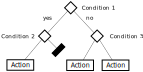
\includegraphics{decisiontree}
			\end{center}
		\end{column}
		\begin{column}{.4\linewidth}
			Complexity: $O(\log_k n)$ \\
			$k$: cardinality of the decision nodes \\
			$n$: number of action nodes
		\end{column}
	\end{columns}
\end{frame}

\begin{frame}[t]{Evaluation Principle}
\begin{itemize}
	\item Start from root decision
	\item For each decision node:
		\begin{enumerate}
			\item Evaluation the condition
			\item Activate the branch according to the condition's value
			\item Select the decision node that is attached to the activated branch
		\end{enumerate}
	\item If an action node is reached, the associated actions are selected
	\item If an iddle node is reached, no action is selected
\end{itemize}
\begin{center}
	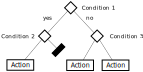
\includegraphics[width=.6\linewidth]{decisiontree}
\end{center}
\end{frame}

\begin{frame}{Types of Decisions}
	\begin{stabularx}{l|X}
		\tabularhead{Condition Type}{Evaluation Principle} \\
		boolean & if true, activate ``yes'' branch, otherwise ``no'' branch \\
		\hline
		enumeration of values & activate the branch associated to the value \\
		\hline
		numeric value & activate the branch associated to a range of values in which the condition value is \\
		\hline
		[3D] vector & activate the branch associated to a range of values in which the vector length is \\
	\end{stabularx}
	
	\hiconbox{Whatever the type of the decisions, they should be simple, i.e. fast to be evaluated}{info-icon}
\end{frame}

\begin{frame}{{Boolean Combination} of Decisions}
	\begin{tabularx}{\linewidth}{XX}
		If C1 \Emph{and} C2 then A1 else A2 & If C1 \Emph{or} C2 then A1 else A2 \\
		\includegraphics[width=.8\linewidth]{decisiontree_and}
		&
		\includegraphics[width=.8\linewidth]{decisiontree_or}
	\end{tabularx}
\end{frame}

\begin{frame}{Knowledge Representation}
	\begin{block}{Direct access to the agent memory}
		\begin{itemize}
			\item Decisions are directly linked to primitive data types
			\item No translation from agent knowledge to decision expressions
		\end{itemize}
	\end{block}
	\begin{alertblock}{Possible Issues}
		\begin{itemize}
			\item Direct access to private data from other characters
			\item Agent implementation-dependent
		\end{itemize}
	\end{alertblock}
	\begin{block}<2>{Possible Solutions}
		To fix these problems, data is insulated inside:
		\begin{itemize}
			\item an enviromnent model, or
			\item a generic agent knowledge representation model.
		\end{itemize}
	\end{block}
\end{frame}

\begin{frame}{Branching Optimization}
	\begin{columns}
		\begin{column}{.5\linewidth}
			\begin{block}{Binary Tree}
				\begin{itemize}
				\item Most decision tree are based on boolean conditions
				\item Easier to optimize (tree balancing)
				\end{itemize}
			\end{block}
			\includegraphics[width=\linewidth]{decisiontree_bin}
		\end{column}
		\begin{column}{.5\linewidth}
			\begin{block}{N-ary Tree}
				\begin{itemize}
				\item Sometimes it is more convenient to have more choices
				\item This structure is flatter:
					\begin{itemize}
						\item only requires one decision
						\item is obviously more efficient
					\end{itemize}
				\end{itemize}
			\end{block}
			\includegraphics[width=\linewidth]{decisiontree_nary}
		\end{column}
	\end{columns}
\end{frame}

\begin{frame}[fragile]{{Pseudo-Code:} Action}
	\begin{sarllisting}[basicstyle=\scriptsize]
abstract class DecisionTreeNode {
	//Recursively walks through the tree
	abstract def makeDecision
}

abstract class Action extends DecisionTreeNode
	def makeDecision {
		return this
	}
}
	\end{sarllisting}
\end{frame}

\begin{frame}[fragile]{{Pseudo-Code:} Binary Decision}
\begin{sarllisting}[basicstyle=\scriptsize]
abstract class BinaryDecision extends DecisionTreeNode {

	protected var trueNode : DecisionTreeNode

	protected var falseNode : DecisionTreeNode

	protected var testValue : Object

	// carries out the test
	abstract def getBranch : DecisionTreeNode
	
	// Recursively walks through the tree
	def makeDecision {
		// Make the decision and recurse based on the result
		var branch = getBranch
		return branch.makeDecision
	}
}
\end{sarllisting}
\end{frame}

\begin{frame}[fragile]{{Pseudo-Code:} Float Range Decision}
\begin{sarllisting}[basicstyle=\scriptsize]
class FloatBinaryDecision extends BinaryDecision {

	var minValue : float

	var maxValue : float

	def getBranch {
		if ((minValue .. maxValue).contains(testValue as float)) {
			return trueNode
		} else {
			return falseNode
		}
	}
}
\end{sarllisting}
\end{frame}

\begin{frame}[fragile]{{Pseudo-Code:} Multi-Branch Decision}
\begin{sarllisting}[basicstyle=\scriptsize]
class MultiDecision extends DecisionTreeNode {

	var children : List<DecisionTreeNode>

	var testValue : Object
	
	// Carries out the test and returns the node to follow
	def getBranch {
		return children.get(testValue as int)
	}
	
	// Recursively runs the algorithm, exactly as before
	def makeDecision {
		var branch = getBranch
		return branch.makeDecision
	}
}
\end{sarllisting}
\end{frame}

\begin{frame}[t]{Balanced or not?}
	\begin{block}{Unbalanced Tree}
			\begin{center}
				\includegraphics[width=.6\linewidth]{decisiontree_unbalanced}
			\end{center}
		\smaller 
		\begin{tabularx}{\linewidth}{@{}XX@{}}
			Best case: 1 decision & Bad case: 6 decisions \\
			Average case: 4 decisions & Complexity: $O(\frac{n}{2})$ \\
		\end{tabularx}
	\end{block}
	\begin{columns}
		\begin{column}{.5\linewidth}
			\begin{block}{Balanced Tree}
				\begin{tabularx}{\linewidth}{@{}XX@{}}
					\raisebox{-.7\height}{\includegraphics[width=\linewidth]{decisiontree_balanced}} &  \smaller Best: 3 \newline
					Bad: 3 \newline
					Average: 3 \newline
					$O(log_2 n)$
				\end{tabularx}
			\end{block}
		\end{column}
		\begin{column}{.5\linewidth}
			\begin{alertblock}<2>{Balanced or not?}
				\begin{itemize}
					\item Balanced tree $\Rightarrow$ theoretically optimal
					\item What about if C1 is almost always true?
					\item Unbalanced tree becomes the best choice
				\end{itemize}
			\end{alertblock}
		\end{column}
	\end{columns}
\end{frame}

\begin{frame}[t]{Pathological Decision Trees}
	\Emph{Avoiding multiple instances of the same action} \\
	$\Rightarrow$ not assigning an action to more than one leaf
	\begin{center}
		\includegraphics[width=.4\linewidth]{decisiontree_pathologic}
	\end{center}
	\alertbox{Do not introduce loops in the tree}
	\hiconbox{The resulting tree is a \Emph{Directed Acyclic Graph} --- DAG}{info-icon}
\end{frame}

\begin{frame}[t]{{Unrealistic} Random Decision}
	\begin{alertblock}{Problem of Decision Trees}
		If decision trees are \emph{run frequently}, reacting to the immediate state of the world, random decisions cause problems
	\end{alertblock}	
	\begin{example}
		\begin{center}
			\includegraphics[width=.4\linewidth]{decisiontree_example}
		\end{center}
		\vspace{-.5cm}
		\begin{itemize}
			\item As long as the agent isn't under attack, stand and patrol behaviours will be chosen randomly
			\item This choice is made at every ``frame'', so that the character will appear to vacillate between standing and moving
		\end{itemize}
	\end{example}
\end{frame}

\begin{frame}{{Stability} in Random Choices}
	\alertbox*{Random decision process needs to become \emph{stable}}
	\begin{itemize}
		\item If there is no relevant change in the world state, there should be no change in decision
		\item But, facing the same state at \emph{very different times}, agent can make different decisions
	\end{itemize}
	\begin{block}{Main Principles}
		\begin{itemize}
			\item Allow random decision to keep track of what it did last time
			\item Random selection should be used again after a timeout was reached
		\end{itemize}
	\end{block}
\end{frame}

\end{graphicspathcontext}

\endinput

	\subsection{Rule-based Decision}
	\begin{graphicspathcontext}{{./chapters/mas/architectures/imgs/},{./chapters/mas/architectures/imgs/auto/},{./chapters/mas/imgs/auto/},\old}

\begin{frame}{What is a Rule-based System?}
	\begin{definitionblock}{Rule-based System (or expert system)}
		Decision-making process that is composed of:
		\begin{itemize}
		\item a database containing knowledge available to the AI
		\item a set of ``if-then'' rules
		\end{itemize}
	\end{definitionblock}
	\vspace{.5cm}
	\begin{block}{General Principle}
		\begin{description}
		\item[Rule activation] Test if a ``if-then'' rule's condition is evaluated to true based on database
		\item[Rule triggering] Rule with true condition is triggered
		\item[Rule firing] Triggered rule may be selected to fire, whereupon its ``then'' component is executed
		\end{description}
	\end{block}
\end{frame}

\begin{frame}[t,fragile]{Fact-base Format}
	\begin{block}{Format of the base of facts}
		\begin{itemize}
			\item Contains the knowledge of an agent
			\item $data = \langle identifier, value \rangle$
		\end{itemize}
	\end{block}
	\begin{example}[Pair Syntax]\ttfamily
		Captain's-weapon = rifle \\
		Johnson's-weapon = machine-gun \\
		Captain's-rifle's-ammo = 36 \\
		Johnson's-machine-gun-ammo = 229
	\end{example}
	\begin{example}[Functional Syntax --- more popular]\ttfamily
		\vspace{-.8em}\begin{sarllisting}[language=lisp,basicstyle=\small]
(Captain
	(Weapon (Rifle (Ammo 36)))
	(Health 65)
	(Position 21, 46, 92))
		\end{sarllisting}\vspace{-3em}
	\end{example}
	\alertbox{Wildcards are allowed: \texttt{(?anyone (Health 0-15))}}
\end{frame}

\begin{frame}{Wildcard Problem}
	\begin{columns}[t]
		\begin{column}{.5\linewidth}
			\begin{block}{Database}\ttfamily
				(Captain (Health 51)) \\
				(Johnson (Health 38)) \\
				(Sale (Health 13)) \\
				(Whisker (Health 15)) \\
				(Radio (Held-by Whisker))
			\end{block}
		\end{column}
		\begin{column}{.5\linewidth}
			\begin{block}{Query}\ttfamily
				(?person (Health 0-15)) \\
				AND \\
				(Radio (Held-by ?person))
			\end{block}
		\end{column}
	\end{columns}
	\begin{block}{Matching}
		\begin{tabularx}{\linewidth}{>{\ttfamily}Xc>{\ttfamily}l}
			(Sale (Health 13)) & $\Rightarrow$ & ?person = Sale \\
			(Radio (Held-by Whisker)) & $\Rightarrow$ & ?person = Whisker \\
		\end{tabularx}
	\end{block}

	\alertbox{But they are expecting to have the same value! No? Really?}
\end{frame}

\begin{frame}{Unification}
	\alertbox{A set of wildcards are matched so that they all refer to the same thing/object/value}
	\begin{definition}[Free variable]
		Each wildcard corresponds to the name a free variable
	\end{definition}
	\begin{definition}[Unification]
		Algorithmic process of solving free variables within larger expressions, in which each occurrence of a free variable must refer to the same value as the other occurrence of the free variable
	\end{definition}
	\begin{example}
		\begin{tabularx}{\linewidth}{>{\ttfamily}Xc>{\ttfamily}l}
			(Whisker (Health 15)) & $\Rightarrow$ & ?person = Whisker \\
			(Radio (Held-by Whisker)) & $\Rightarrow$ & ?person = Whisker \\
		\end{tabularx}
	\end{example}
\end{frame}

\begin{frame}{Database Matching}
	\alertbox*{Condition (or pattern) consists of facts identical to those on database, combined with boolean operators}
	\begin{columns}[t]
		\begin{column}{.5\linewidth}
			\begin{block}{Database}\ttfamily
				(Captain (Health 51)) \\
				(Johnson (Health 38)) \\
				(Sale (Health 42)) \\
				(Whisker (Health 15))
			\end{block}
		\end{column}
		\begin{column}{.5\linewidth}
			\begin{block}{Rule}\ttfamily
				IF (Whisker (Health 0)) \\
				AND (Radio Whisker) \\
				AND (?a (Health >0)) \\
				THEN \\
				$\ominus$ (Radio Whisher) \\
				$\oplus$ (Radio ?a)
			\end{block}
		\end{column}
	\end{columns}
	\vspace{.5cm}
	\alertbox*{No match from database $\Rightarrow$ nothing to do}
\end{frame}

\begin{frame}[t]{Database Matching \insertcontinuationtext}
\begin{columns}[t]
	\begin{column}{.5\linewidth}
		\begin{block}{Database}\ttfamily
			(Fuel 1500) \\
			(Distance-to-Base 100) \\
			(Enemies (Guy1 42) \\
			       (Guy2 21)) \\
			(Action Patrolling)
		\end{block}
		\begin{block}{New Database}\ttfamily
			(Fuel 1500) \\
			(Distance-to-Base 100) \\
			(Enemies (Guy1 42) \\
			(Guy2 21)) \\
			(Action (Attack Guy2))
		\end{block}
	\end{column}
	\begin{column}{.5\linewidth}
		\begin{block}{Rule}\ttfamily
			IF (Action Patrolling) \\
			AND (Enemies (list ?a)) \\
			AND ?s = (min-pair-b ?a)
			THEN \\
			$\ominus$ (Action Patrolling) \\
			$\oplus$ (Action (Attack ?s))
		\end{block}
		\ttfamily
		?a = ((Enemy1 42) (Enemy2 21)) \\
		?d = 21 \\
		?s = Guy2
	\end{column}
\end{columns}
\end{frame}

\begin{frame}{Rule Application Methods}
	\begin{block}{Forward Chaining}
		\begin{itemize}
		\item Starts with a known database of information
		\item Repeatedly applies rules that change the database content
		\end{itemize}
	\end{block}
	\begin{block}{Backward Chaining}
		\begin{itemize}
			\item Starts with a given piece of knowledge (found in database) as a goal
			\item Find rules matching the goals to reach
			\item Look conditions to determine how they may be triggered
			\item Actions that may trigger conditions are new sub-goals to reachs
			\item Optionally, loop with sub-goals and goals until no more rule is usable
		\end{itemize}
	\end{block}
\end{frame}

\begin{frame}{Naive Algorithm}
	\begin{block}{Inputs}
		\begin{itemize}
			\item Not-empty database
			\item Set of rules
		\end{itemize}
	\end{block}
	\begin{block}{Algorithm}
		\begin{itemize}
			\item Rules are applied in iterations
			\item Each rules is checked to determine if it is triggering on current database knowledge
			\item \Emph{First triggered rule is fired}, and rule's action is executed
		\end{itemize}
	\end{block}
\end{frame}

\begin{frame}[fragile]{{Pseudo-Code:} Database}
\begin{sarllisting}[basicstyle=\scriptsize]
/* According to the format of the database rules, the database
 * is a kind of tree.
 */
interface Database extends Iterable<DataNode> {

	// Defining the node into a tree
	abstract class DataNode {
		var identifier : String
	}
	
	// Defining a non-leaf node
	class DataGroup extends DataNode {
		var children : List<DataNode>
	}
	
	// Defining a leaf node
	class Datum extends DataNode {
		var value : Object
	}
	
}
\end{sarllisting}
\end{frame}

\begin{frame}[fragile]{{Pseudo-Code:} Rule}
\begin{sarllisting}[basicstyle=\scriptsize]
interface Rule {

	/* The IF-clause is used by the algorithm and is
	 * defined in the following slides
	 */
	def getIfClause : IfClauseExpression

	/* This function defines the action to run if
	 * the IF-clause matchs.
	 *
	 * @param bindings the values associated to the wildcards
	 */
	def action(bindings : Map<String, Object>) 

}
\end{sarllisting}
\end{frame}

\begin{frame}[fragile]{{Pseudo-Code:} If-Clause Expression}
\begin{sarllisting}[basicstyle=\scriptsize]
abstract class IfClauseExpression
	/* Function that permits to match this clause to the
	 * content of a database.
	 * The "bindings" parameter is both in input and
	 * output, when a part of the clause matches a
	 * wildcard, it is added to the bindings.
	 */
	def matches(database : Database,
			bindings : Map<String, Object>) : boolean {
		// Go through each item in the database
		for (item : database) {
			if (matchesItems(item, bindings))
				return true
		}
		return false
	}

	abstract def matchesItems(item : DataNode, bindings : Map<String, Object>) : boolean
}
\end{sarllisting}
\end{frame}

\begin{frame}[t,fragile]{{Pseudo-Code:} Data Matcher}
\begin{sarllisting}[basicstyle=\scriptsize]
/* The atomic part of a IF-clause expression is
 * represented by the DatumMatch class.
 */
class DatumMatch extends IfClauseExpression {

	/* Datum to match in the database, or an identifier
	 * starting with "?" to represent a wildcard
	 */
	var identifier : String

	// Range of values to match
	var minValue : Object
	var maxValue : Object

	def matchesItems(item : DataNode,
			bindings : Map<String, Object>) {
		// Is the item of the same type?
		if (!(item instanceof Datum)) return false

		// Does the identifier match?
		if (!identifier.isWildcard
				&& identifier != item.identifier)
			return false
\end{sarllisting}
\end{frame}

\begin{frame}[fragile]{{Pseudo-Code:} Data Matcher \insertcontinuationtext}
\begin{sarllisting}[basicstyle=\scriptsize]
		// Does the value fit?
		if ((minValue .. maxValue).contains(item.value) {

			// Do we need to add to the bindings list?
			if (identifier.isWildcard) {
				bindings += identifier => item
			return true
		} else {
			return false
		}
	}
}
\end{sarllisting}
\end{frame}

\begin{frame}[fragile]{{Pseudo-Code:} Boolean Matcher}
\begin{sarllisting}[basicstyle=\scriptsize]
class AndMatch extends IfClauseExpression {

	// Two operands
	var match1 : IfClauseExpression
	var match2 : IfClauseExpression

	def matches(database : Database,
			bindings : Map<String, Object>) : boolean {
		// True if we match both if-matches
		return match1.matches(database, bindings)
			&& match2.matches(database, bindings)
	}

}
\end{sarllisting}
\end{frame}

\begin{frame}[t,fragile]{{Pseudo-Code:} Group Matcher}
\begin{sarllisting}[basicstyle=\scriptsize]
/* A data group test will match a database data group
 * if its identifier matches and if all its children
 * match at least one child of the database group
 * Example:    (?anyone (Health 0-54))
 *          on (Captain (Health 43) (Ammo 140))
 *          should match
 */
class GroupMatch extends IfClauseExpression {

	var identifier : String

	var children : List<IfClauseExpression>

	def matchesItems(item : DataNode,
			bindings : Map<String, Object>) : boolean {

		// Is the item the same type?
		if (!(item instanceof DataGroup)) return false

		// Does the identifier match?
		if (!identifier.isWildcard
				&& identifier != item.identifier)
			return false
\end{sarllisting}
\end{frame}

\begin{frame}[fragile]{{Pseudo-Code:} Group Matcher \insertcontinuationtext}
\begin{sarllisting}[basicstyle=\scriptsize]
		// Is every child present?
		for (child : children) {
			// Use the children of the item as if they
			// were a database and call matches recursively
			if (!child.matches(item.children))
				return false
		}

		// We have matched all the children

		// Do we need to add to the bindings list?
		if (identifier.isWildcard) {
			bindings += identifier => item
		}
		return true
	}
}
\end{sarllisting}
\end{frame}

\begin{frame}[fragile]{{Pseudo-Code:} Rule System}
\begin{sarllisting}[basicstyle=\scriptsize]
class RuleBasedSystem {

	def iteration(database : Database, rules : List<Rule>) {
		// Check each rule in turn
		for (rule : rules) {
			// Create the empty set of bindings
			var bindings = #{}

			// Check for triggering
			if (rule.ifClause.matches(database, bindings)) {
				// Fire the rule
				rule.action(bindings)
				// Exit: we're done for this iteration
				return
			}
		}
		
		// If we get here, we've had no match, we could
		// use a fallback action, or simply do nothing
	}
}
\end{sarllisting}
\end{frame}

\begin{frame}{Rule Arbitration}
	\alertbox{How to manage rules that trigger at the same time?}
	\vspace{.5cm}
	\alertbox*{Only a single could be fired within a set of triggered rules}
	\vspace{.5cm}
	\begin{alertblock}{Naive Arbitration}
			\begin{itemize}
				\item First triggered rule is allowed to fire
				\item Fine as long as the rules are arranged in order of priority
			\end{itemize}
	\end{alertblock}
	\begin{example}[of problem]
		\begin{itemize}
		\item If the rule does not change the content of the database
		\item If no external changes are imposed, then the same rule will continue to fire every time the system is run.
		\end{itemize}
	\end{example}
\end{frame}

\begin{frame}{{Rule Arbitration:} Least Recently Used}
	\begin{block}{Principle}
		Use the least recently used rule
	\end{block}
	\begin{block}{How?}
		\begin{itemize}
			\item FIFO linked list of the rules
			\item When a rule is fired, it is removed from its position and added to the end
		\end{itemize}
	\end{block}
	\begin{alertblock}{Advantages}
		\begin{itemize}
			\item No ``loop'' issue
			\item Each rule has the opportunity to fire
			\item $O(\frac{n}{2})$
		\end{itemize}
	\end{alertblock}
\end{frame}

\begin{frame}{{Rule Arbitration:} Random Rule}
	\begin{block}{Principle}
		Select randomly within the set of triggered rules
	\end{block}
	\begin{block}{How?}
		\begin{itemize}
			\item Loop on all rules to detect the triggered ones
			\item Random selection with the set of triggered rules
		\end{itemize}
	\end{block}
	\begin{alertblock}{Disadvantage}
		\begin{itemize}
			\item $O(n)$, where $n$ is the number of rules
		\end{itemize}
	\end{alertblock}
\end{frame}

\begin{frame}{{Rule Arbitration:} Most Specific Condition}
	\begin{definition}[Rule Specialization]
	\begin{itemize}
		\item When conditions are very easy to meet, or database regularly triggers it, then they are general rules
		\item When conditions are hard to fulfill or less triggered by the system, then they are specific rules
	\end{itemize}
	\end{definition}
	\begin{block}{Principle}
		More specific rules should be preferred over more general rules
	\end{block}
	\begin{block}{How?}
		\begin{itemize}
			\item From boolean conditions, the number of clauses is a good indicator of the specificity of the rule
			\item Arbiter is the same as ``first applicable'' arbiter $\Rightarrow$ Rules are ordered \Emph{offline}
		\end{itemize}
	\end{block}
\end{frame}

\begin{frame}{{Rule Arbitration:} Dynamic Priority}
\begin{block}{Principle}
	Associate a priority value to each rule in order to select the most suitable rule in a specific context
\end{block}
\begin{block}{How?}
	\begin{itemize}
		\item Rules are arranged in order of decreasing priority
		\item First triggered rule is fired
	\end{itemize}
\end{block}
	\begin{alertblock}{Disadvantage}
	\begin{itemize}
		\item $O(\frac{n}{2} + n.\log_2(n))$, where $n$ is the number of rules
	\end{itemize}
\end{alertblock}
\end{frame}

\begin{frame}{RETE Algorithm}
	\begin{itemize}
		\item RETE algorithm is an AI industry standard for matching rules against a database
		\vspace{.5cm}
		\item One of the fastest algorithm in the market
		\vspace{.5cm}
		\item Not commonly used, due to patent restrictions and private implementation
		\vspace{.5cm}
		\item Inside most of the commercial expert systems, with specific and complex optimizations
	\end{itemize}
\end{frame}

\begin{frame}{The RETE}
	\begin{definition}Directed Acyclic Graph composed of:
		\begin{description}
			\item[Pattern Node] single condition term that may be used in one or more rules
			\item[Join Node] combination of nodes with the ``and'' boolean operator
			\item[Rule Node] name of the firable rule
			\item[Edge] association between terms in a rule's condition
			\item[Path] complete condition expression for a rule
		\end{description}
	\end{definition}
	\vspace{.5cm}
	\alertbox*{Each node contains a list of all the matching facts against the database}
\end{frame}

\begin{frame}{RETE Example}
	\begin{columns}
		\begin{column}{.6\linewidth}
			\smaller\smaller
			\begin{tabularx}{\linewidth}{|X|}
			\hline
			\textbf{Swap Radio Rule:} \\
			\ttfamily
			IF (?person1 (Health $<$15)) AND \\
			(Radio (Held-by ?person1)) AND \\
			(?person2 (Health $>$ 45)) \\
			THEN \\
			$\ominus$ (Radio (Held-by ?person1)) \\
			$\oplus$ (Radio (Held-by ?person2)) \\
			
			\hline
			\textbf{Change Backup Rule:} \\
			\ttfamily
			IF	(?person1 (Health $<$15)) AND \\
			(?person2 (Health $>$45)) AND \\
			(?person2 (IsCovering ?person1)) \\
			THEN \\
			$\ominus$ (?person2 (IsCovering
			?person1)) \\
			$\oplus$ (?person1 (IsCoveting
			?person2)) \\
			\hline
			\end{tabularx}
		\end{column}
		\begin{column}{.4\linewidth}
			\includeanimatedfigure[width=\linewidth]{rete1}
		\end{column}
	\end{columns}
\end{frame}

\begin{frame}{{Key Elements} of the RETE Algorithm}
	\begin{itemize}
		\item Start from right
		\vspace{.5cm}
		\item Try to find triggered rules (at the left)
		\vspace{.5cm}
		\item If wildcard, node gives variable ``bindings''
		\vspace{.5cm}
		\item Pattern nodes records matching facts for incremental updating
		\vspace{.5cm}
		\item \Emph{Notice that rather than finding a match, we find all matches}
	\end{itemize}
\end{frame}

\begin{frame}{{RETE Example:} Rule activitation}
	\centering\includeanimatedfigure[width=.85\linewidth]{rete2}
\end{frame}

\begin{frame}{Fact Removal}
\begin{itemize}
	\item Removal request identifies the fact that has been removed
	\item Removal request is sent to each pattern node
	\item If pattern node has the fact, then \begin{itemize}
		\item the match is removed
		\item the removal request is forward to any join nodes
	\end{itemize}
	\item If join node has the fact, then \begin{itemize}
		\item the match is removed
		\item the removal request is forward to any join nodes
	\end{itemize}
	\item If rule node has the fact, then it is desactivated
	\item If any node doesn't have the fact, then it does nothing
\end{itemize}
\end{frame}

\begin{frame}{{RETE Example:} Fact Removal}
	\centering\includeanimatedfigure[width=.85\linewidth]{rete3}
\end{frame}

\begin{frame}{Fact Addition}
\begin{itemize}
	\item Adding a fact is very similar to removing one.
	\item If pattern node matches, then it updates its bindings and notifies the join nodes
	\item If it is a new fact for join node, it adds it to its bindings and notifies nodes
	\item If is ia a new fact for rule node, it updates its bindings and change its activation status.
	\item If the fact doesn't update the node, then there is no need to pass the addition request to the next nodess
\end{itemize}
\end{frame}

\begin{frame}{{RETE Example:} Fact Addition}
	\centering\includeanimatedfigure[width=.85\linewidth]{rete4}
\end{frame}

\begin{frame}{{RETE Example:} Remove+Add}
	\centering\includeanimatedfigure[width=.85\linewidth]{rete5}
\end{frame}

\end{graphicspathcontext}

\endinput

	\subsection{State Machine}
	\begin{graphicspathcontext}{{./chapters/mas/architectures/imgs/},{./chapters/mas/architectures/imgs/auto/},{./chapters/mas/imgs/auto/},\old}

\begin{frame}{What is a State of an Agent?}
	\smaller
	\begin{definitionblock}{State}
	\emph{Description of the status} of a system that is waiting to execute a transition.
	\end{definitionblock}
	\begin{example}[State]
		\begin{description}
			\item[In an object $o$] \emph{named} set of values of all the fields of $o$, including the fields in the super classes
			\item[In an agent $a$] \emph{named} union of fields' values and states of data structures within the agent 
		\end{description}
	\end{example}
	\begin{definitionblock}{Transition}
	Set of actions to be executed when a condition is fulfilled or when an event is received. 
	\end{definitionblock}
	\begin{definitionblock}{Action}
	Description of changes of fields' values that cause a state change. 
\end{definitionblock}
\end{frame}

\begin{frame}{What is a Finite State Machine?}
	\begin{definitionblock}{Finite State Machine (FSM)}
		\begin{itemize}
		\item Mathematical model of computation in which the machine can be in exactly one of a finite number of states at any given time
		\item FSM can change from one state to another in response to some inputs
		\item $FSM = \langle S, s_0, T \rangle$ \\
			$S$: finite set of all the reachable states \\
			$s_0$: initial state of the machine \\
			$T : S \rightarrow S$, finite set of transitions 
		\end{itemize}
	\end{definitionblock}
\end{frame}

\figureslide[width=.6\linewidth]{Example of the Cleaning Robot}{fsm_cleaner}

\begin{frame}{FSM for Agents}
	\includeanimatedfigure[width=\linewidth]{fsm_foragent}
\end{frame}

\begin{frame}[fragile]{{Pseudo-Code:} State and Transition}
	\begin{sarllisting}[basicstyle=\scriptsize]
interface State {
	def getInActions : List<Action>
	def getEnterActions : List<Action>
	def getExitActions : List<Action>
	def getTransitions : List<Transition>
}

interface Transition {
	def isTriggered : boolean
	def getTargetState : State
	def getActions : List<Action>
}
	\end{sarllisting}
\end{frame}

\begin{frame}[fragile]{{Pseudo-Code:} State Machine}
\begin{sarllisting}[basicstyle=\scriptsize]
class StateMachine {
	// Holds a list of states for the machine
	var states : List<State>
	// Holds the initial state
	var initialState : State
	// Holds the current state
	var currentState = initialState

	// Checks and applies transitions
	def update : List<Action> {
		// Assume no transition is triggered by default
		var triggeredTransition : Transition = null
		// Search for the first transition that triggers
		val iterator = currentState.transitions.iterator
		while (iterator.hasNext && triggeredTransition === null) {
			val transition = iterator.next
			if (transition.isTriggered) {
				triggeredTransition = transition
			}
		}
\end{sarllisting}
\end{frame}

\begin{frame}[fragile]{{Pseudo-Code:} State Machine \insertcontinuationtext}
\begin{sarllisting}[basicstyle=\scriptsize]
		// Check if we have a transition to fire
		if (triggeredTransition !== null) {
			// Find the target state
			var targetState = triggeredTransition.targetState

			var actions = currentState.exitActions.clone
			actions += triggeredTransition.actions
			actions += targetState.entryActions

			currentState = targetState

			return actions
		} else {
			// Just return the current state's actions
			return currentState.inActions
		}
	}
}
\end{sarllisting}
\end{frame}

\begin{frame}{Performance Analysis}
	\begin{itemize}
		\item $O\left(n\times(1+m)\right)$ in memory
		\item $O(m)$ in time
		\item Where:
			\begin{itemize}
				\item $n$ is the number of states
				\item $m$ is the number of transitions per state
				\item Actions' list building is negligible
			\end{itemize}
		\vspace{1cm}
		\item Possible expensive functions:
			\begin{itemize}
				\item \code{State.getTransitions}
				\item \code{State.getTargetState}
			\end{itemize}
	\end{itemize}
\end{frame}

\begin{frame}{FSM in the Agent Lifecycle}
	\begin{center}
		\includegraphics[width=.8\linewidth]{fsm_inagent}
	\end{center}
	\begin{columns}
		\begin{column}{.5\linewidth}
			\begin{block}{Current state is compatible with agent's State-of-Mind}
				\code{currentState == determineState(knowledge)}
				\begin{itemize}
					\item Use of the FSM
				\end{itemize}
			\end{block}
		\end{column}
		\begin{column}{.5\linewidth}
			\begin{alertblock}{Current state is incompatible with agent's State-of-Mind}
				\code{currentState != determineState(knowledge)}
				\begin{itemize}
					\item Force FSM current state?
					\item Continue with FSM current state?
				\end{itemize}
			\end{alertblock}
		\end{column}
	\end{columns}
\end{frame}

\begin{frame}[t,fragile]{Hard-Coded FSM}
	\begin{itemize}
	\item Few years back, almost all state machines were hard-coded
	\item Rules for transitions and execution of actions were part of the simulator code itself
	\vspace{.25cm}
	\item[$\oplus$] Very efficient implementation
	\item[$\ominus$] Static definition of the states and the transitions
	\end{itemize}
	\vspace{-.5cm}
	\begin{columns}
		\begin{column}[t]{.5\linewidth}
			\begin{sarllisting}[basicstyle=\tiny]
enum State {
	PATROL, DEFEND, SLEEP
}

class PatrollerFSM {
	var currentState = State::SLEEP
	
	def update(k : Knowledge)
			: List<Action> {
		switch(currentState) {
			case PATROL: {
				if (k.seePlayer) {
					currentState = DEFEND
					return #[]
				} else if (k.tired) {
					currentState = SLEEP
					return #[]
				} else {
			\end{sarllisting}
		\end{column}
		\begin{column}[t]{.5\linewidth}
			\begin{sarllisting}[basicstyle=\tiny]
					return #[RANDOM_MOVE]
				}
			}
			case DEFEND: {
				if (!k.seePlayer) {
					currentState = PATROL
					return #[]
				} else {
					return #[FIRE_GUN]
				}
			}
			case SLEEP: {
				if (!k.tired) {
					currentState = PATROL
				}
				return #[]
			}
		}
	}
}
\end{sarllisting}
		\end{column}
	\end{columns}
\end{frame}

\begin{frame}{Complex or Alternate Behaviors}
	\alertbox{How to express alternate behaviors with a FSM?}
	\begin{example}[Cleaning Robot]
		\begin{center}
			\includegraphics[width=.5\linewidth]{fsm_cleaner}
		\end{center}
	\end{example}
	\alertbox*{How introducing power down feature for the robot?}
\end{frame}

\figureslide{{Bad Answer:} cannot resume alternate state}{fsm_cleaner_bad0}

\figureslide{{Bad Answer:} duplication of states}{fsm_cleaner_bad1}

\figureslide{{Good Answer:} hierarchical state machine}{fsm_cleaner_good}

\begin{frame}[t,fragile]{{Pseudo-Code:} Abstract HFSM}
\begin{sarllisting}[basicstyle=\scriptsize]
class UpdateResult {
	var actions : List<Action>
	var transitions : List<Transition>
	var level : int
}

abstract class AbstractHFSM {

	def getActions : List<Action> {
		#[]
	}

	def update : UpdateResult {
		new UpdateResult => [
			actions = getActions
			transition = null
			level = 0
		]
	}

	abstract def getStates : List<AbstractHFSM>
}
\end{sarllisting}
\end{frame}

\begin{frame}[fragile]{{Pseudo-Code:} State and Transition}
	\begin{columns}
		\begin{column}{.5\linewidth}
			\begin{sarllisting}[basicstyle=\scriptsize]
class State extends AbstractHFSM { 
	def getStates {
		// If we're just a state
		// then the stack is just us
		#[ this ]
	}

	// As in the standard FSM
	// implementation...
	def getActions {...}
	def getEnterActions {...}
	def getExitActions {...}
	def getTransitions {...}
}
			\end{sarllisting}
		\end{column}
		\begin{column}{.5\linewidth}
			\begin{sarllisting}[basicstyle=\scriptsize]
class Transition {
	// Returns the different in
	// levels of the hierarchy
	// from the source to the target
	// of the transition
	def getLevel : int {...}

	// As in the standard FSM implementation...
	def isTriggered {...}
	def getTargetState {...}
	def getActions {...}
}
			\end{sarllisting}
		\end{column}
	\end{columns}
\end{frame}

\begin{frame}[t,fragile]{{Pseudo-Code:} HFSM}
	\begin{sarllisting}[basicstyle=\scriptsize]
class HierarchicalFiniteStateMachine extends AbstractHFSM {
	// List of states at this level of the hierarchy
	var states : List<State>

	// The initial state for when the machine has to current state
	var initialState : State

	// The current state of the machine
	var currentState = initialState

	// Gets the current state stack
	def getStates : List<AbstractHFSM>
		this.currentState?.getStates
	}
	\end{sarllisting}
\end{frame}

\begin{frame}[t,fragile]{{Pseudo-Code:} HFSM \insertcontinuationtext}
	\begin{sarllisting}[basicstyle=\scriptsize]
	// Recursively updates the machine
	def update : UpdateResult {
		// If we're in no state, use the initial state
		if (currentState === null) {
			currentState = initialState
			return currentState.getEntryActions
		}

		// Try to find a transition in the current state
		var triggeredTransition = null
		val iterator = currentState.transitions.iterator
		while (iterator.hasNext &&
				triggeredTransition === null) {
			val transition = iterator.next
			if (transition.isTriggered)
				triggeredTransition = transition
		}
	\end{sarllisting}
\end{frame}

\begin{frame}[t,fragile]{{Pseudo-Code:} HFSM \insertcontinuationtext}
	\vspace{-.25cm}
	\begin{sarllisting}[basicstyle=\scriptsize]
		// If we're found one, make a result structure for
		// it
		var result = UpdateResult
		if (triggeredTransition !== null) {
			result = new UpdateResult => [
				actions = #[]
				transition = triggeredTransition
				level = triggeredTransition.level
			]
		} else {
			// Otherwise recurse down for a result
			result = currentstate.updaTransitionte
		}

		// Check if the result contains a transition
		if (result.transition !== null) {
			// Act based on its level
			if (result.level === 0) {
				// Its on our level: honor it
				targetState = result.transition.targetState
				result.actions += currentState.exitActions
				result.actions += result.transition.actions
				result.actions += targetState.enterActions
	\end{sarllisting}
\end{frame}

\begin{frame}[t,fragile]{{Pseudo-Code:} HFSM \insertcontinuationtext}
	\vspace{-.25cm}
	\begin{sarllisting}[basicstyle=\scriptsize]
				// Set our current state
				currentState = targetState
				// Add our normal action (we may be a state)
				result.actions += getActions
				
				// Clear the transition, so nobody else does it
				result.transition = null
			} else if (result.level > 0) {
				// Its destined for a higher level
				// Exit our current state
				result.actions += currentState.exitActions
				currentState = null
				// Decrease the number of levels to go
				result.level --
			} else {
				// It needs to be passed down
				targetState = result.transition.targetState
				targetMachine = targetState.parent
				result.actions += result.transition.actions
				result.actions += targetMachine.updateDown(
				targetState, -result.level)
				// Clear the transition, so nobody else does it
				result.transition = null
			}
	\end{sarllisting}
\end{frame}

\begin{frame}[t,fragile]{{Pseudo-Code:} HFSM \insertcontinuationtext}
	\begin{sarllisting}[basicstyle=\scriptsize]
		} else {
			// We can simply do our normal action
			result.actions += getActions
		}

		// Return the accumulated result
		return result
	}

	// Recurses up the parent hierarchy, transitioning
	// into each state in turn for the given number of
	// levels
	def updateDown(state : AbstractHFSM, level : int) {
		// if we're at top elvel, continue recursing
		if (level > 0) {
			// Pass ourself as the transition state to our parent
			actions = parent.updateDown(this,level - 1)
		} else {
			// Otherwise we have no action to add to
			actions = #[]
		}
	\end{sarllisting}
\end{frame}

\begin{frame}[t,fragile]{{Pseudo-Code:} HFSM \insertcontinuationtext}
	\begin{sarllisting}[basicstyle=\scriptsize]
		// If we have a current state, exit it
		if (currentState !== null)
			actions += currentState.exitActions

		// Move to the new state, and return all the actions
		currentState = state
		actions += state.getEnterActions
		return actions
	}
}
	\end{sarllisting}
\end{frame}

\begin{frame}[t,fragile]{{Pseudo-Code:} Sub-machine}
	\begin{sarllisting}[basicstyle=\scriptsize]
class SubMachineState
		extends State, HierarchicalStateMachine

	// Route get action to the state
	def getActions {
		State::getActions
	}

	// Route update to the state machine
	def update {
		HierarchicalFiniteStateMachine.update
	}

	// We get states by adding ourself to our active children
	def getStates {
		if (currentState !== null)
			return #[this] + currentState.states
		else
			return #[this]
	}
}
	\end{sarllisting}
\end{frame}

\begin{frame}[t]{Combining Decision Trees and State Machines}
	\begin{itemize}
	\item Decision trees are an efficient way of matching series of conditions
	\item Decision trees and FSM could be combined by replacing transitions in a FSM by a decision tree.
	\end{itemize}
	\begin{center}
		\includegraphics[width=.8\linewidth]{fsm_dt}
	\end{center}
	\alertbox{Is it different than a composed boolean condition? \\
	$\Rightarrow$ it may be optimization for avoiding evaluation of the same boolean sub-expressions \\
	$\Rightarrow$ dynamic building of the transition}
\end{frame}

\end{graphicspathcontext}

\endinput

	\subsection{Goal-Oriented Behavior}
	\begin{frame}{What is a Goal?}
	\begin{definitionblock}{Goal}
		Part of the state of the system (environment or the agent itself) that should be reached by the agent \\
		$g \in G = \langle i, S \rangle$ \\
		$i$: insistence value of the goal (level of importance) \\
		$S$: set of actions associated to the goal
	\end{definitionblock}
	
	\begin{itemize}
	\item Agent could have one or more goals
	\item Agent has to fullfil the goal or to reduce its insistence
	\item To reach a goal or reduce its insistence, agent must apply an action
	\end{itemize}
\end{frame}

\begin{frame}{What is an Action?}
	\begin{definitionblock}{Action}
		Definition of the incrementation or decrementation values for goals insistences. \\
		$a \in A : G \rightarrow \mathbb{R}$ \\
	\end{definitionblock}
	\begin{itemize}
	\item Can be hard-coded, or given by several environmental objects
	eg., a door provides the actions ``open'', ``lock''
	\item Availability depends on:
		\begin{itemize}
		\item the current state of the environment
		\item the perceived objects
		\end{itemize}
	\end{itemize}
\end{frame}

\begin{frame}{{Action Selection:} Most-Insistense Algorithm}
	\begin{block}{Principle}
		Choose the action that corresponds to the \textcolor<2>{CIADmagenta}{most pressing goal}, and that provides the \textcolor<3>{CIADmagenta}{largest decrease in insistence}
	\end{block}
	\begin{example}[at time \only<1-3>{$t$}\only<4>{$t+1$}]
		\begin{tabularx}{\linewidth}{lXXr}
			Goal: & Hunger & = \only<1-3>{4}\only<4>{\textcolor{CIADmagenta}{1}} & \only<2,4>{\textcolor{CIADmagenta}{$\Leftarrow$}} \\
			Goal: & Tired & = 3 & \\
			Action: & Get-Raw-Food & Hunger: -3 & \only<3>{\textcolor{CIADmagenta}{$\Leftarrow$}} \\
			Action: & Get-Snack & Hunger: -2 & \\
			Action: & Sleep-In-Bed & Tired: -4 & \\
			Action: & Sleep-On-Sofa & Tired: -2 & \\
		\end{tabularx}
	\end{example}
\end{frame}

\begin{frame}[fragile]{{Pseudo-Code:} Goal and Action}
	\begin{sarllisting}[basicstyle=\scriptsize]
interface Goal {

	def getName : String

	def getInsistence : float

	def setInsistence(newInsistence : float)

}


interface Action {

	def getName : String

	def getGoalChange(goal : Goal) : float

}
\end{sarllisting}
\end{frame}

\begin{frame}[fragile]{{Pseudo-Code:} Choose Goal}
\begin{sarllisting}[basicstyle=\scriptsize]
class GoalOrientedBehaviour {

	def chooseAction(
			actions : List<Action>,
			goals : List<Goal>) {

		// Find the goal to try and fulfill
		var iterg = goals.iterator
		topGoal = iterg.next

		while (iterg.hasNext) {
			val goal = iterg.next
			if (goal.insistence > topGoal.insitence)
				topGoal = goal
		}
\end{sarllisting}
\end{frame}

\begin{frame}[t,fragile]{{Pseudo-Code:} Choose Action}
\begin{sarllisting}[basicstyle=\scriptsize]
		// Find the best action to take
		var itera = actions.iterator
		bestAction = itera.next
		bestUtility = - bestAction.getGoalChange(topGoal)
		while (itera.hasNext) {
			val action = itera.next

			// We invert the change because a low change value
			// is good (we want to reduce the insistence for
			// the goal) but utilities are typically scaled so
			// high values are good
			utility = - action.getGoalChange(topGoal)

			// We look for the lowest change (highest utility)
			if (utility > bestUtility) {
				bestUtility = utility
				bestAction = action
			}
		}

		// Return the best action to be carried out
		return bestAction
	}
}
\end{sarllisting}
\end{frame}

\begin{frame}{Complexity Analysis}
	\begin{block}{In time}
		$O(g+a)$ \\
		$g$: number of goals \\
		$a$: number of possible actions
	\end{block}
	\begin{block}{Memory footprint}
		$O(g + a)$ \\
		$g$: number of goals \\
		$a$: number of actions
	\end{block}
\end{frame}

\begin{frame}{{Most-Insistense Algorithm:} Bad Side-Effects}
\begin{example}
	\begin{tabularx}{\linewidth}{lXX}
		Goal: & Hunger & = 4 \\
		Goal: & Urination & = 3 \\
		Action: & Drink-Soda & Hunger:~-2; Urination:~+3 \\
		Action: & Visit-Bathroom & Urination: -4 \\
	\end{tabularx}
\end{example}
\alertbox*{Natural Human Behavior: Human Being may not select the Drink-Soda action because it increase the Bathroom's insistence with a high rate}
\alertbox{But the simple selection algorithm select Drink-Soda, before Visit-Bathroom}
\end{frame}

\begin{frame}{{Solution:} Overall Utility}
	\begin{definition}[Discontentment of the agent]
		\begin{itemize}
			\item Discontentment is a global value for an agent that indicates the level of contentment of the agent regarding its general state
			\item Higher are the goals' insistences, higher is the agent's discontenment
			\item Agent aims at reducing its discontentment
			\item $dis = \sum_{g \in G} \left(insistence_g\right)^2$
		\end{itemize}
	\end{definition}
	\begin{itemize}
		\item In Research literature, discontentment is also known as ``energy''
		\item This concept of energy is also used in learning algorithms
	\end{itemize}
\end{frame}

\begin{frame}{{Discontentment Algorithm:} Example}
\begin{example}[at time \only<-3>{$t$}\only<4>{$t+1$}]
	\begin{tabularx}{\linewidth}{lXXr}
		Goal: & Hunger & = \only<-3>{4}\only<4>{\textcolor{CIADmagenta}{4}} & \\
		Goal: & Urination & = \only<-3>{3}\only<4>{\textcolor{CIADmagenta}{0}} & \\
		Action: & Drink-Soda & Hunger: -2; & \\
		& & Urination: +3 & \\
		\only<2>{\textcolor{CIADmagenta}{$\Rightarrow$}} & \only<2>{\textcolor{CIADmagenta}{Hunger=2}}& \only<2>{\textcolor{CIADmagenta}{Urination=6}} & \only<2>{\textcolor{CIADmagenta}{dis=40}} \\
		Action: & Visit-Bathroom & Urination: -4 & \\
		\only<2-3>{\textcolor{CIADmagenta}{$\Rightarrow$}} & \only<2-3>{\textcolor{CIADmagenta}{Hunger=4}}& \only<2-3>{\textcolor{CIADmagenta}{Urination=0}} & \only<2-3>{\textcolor{CIADmagenta}{dis=16}} \\
	\end{tabularx}
\end{example}
\end{frame}

\begin{frame}[fragile]{{Discontentment Pseudo-Code:} Goal and Action}
\begin{sarllisting}[basicstyle=\scriptsize]
interface Goal {
	def getName : String

	def getInsistence : float
	def setInsistence(newInsistence : float)

	def discontentment(insistenceValue : float) : float {
		insistenceValue ** 2
	}
}

interface Action {

	def getGoalChange(goal : Goal) : float

}
\end{sarllisting}
\end{frame}

\begin{frame}[t,fragile]{{Discontentment Pseudo-Code:} Best Action}
\begin{sarllisting}[basicstyle=\scriptsize]
class GoalOrientedBehaviour2 {

	def chooseAction(
			actions : List<Action>,
			goals : List<Goal>) {

		// Go through each action, and calculate the discontentment
		val itera = actions.iterator
		var bestAction = itera.next
		var bestValue = bestAction.calculateDiscontentment(goals)
		while (itera.hasNext) {
			val action = itera.next
			var value = action.calculateDiscontentment(goals)
			if (value < bestValue) {
				bestValue = value
				bestAction = action
			}
		}

		// Return the best action
		return bestAction
	}
\end{sarllisting}
\end{frame}

\begin{frame}[fragile]{{Discontentment Pseudo-Code:} Discontentment}
\begin{sarllisting}[basicstyle=\scriptsize]
	def calculateDiscontentment(
			action : Action,
			goals : List<Goal>) {
	
		// Keep a running total
		var discontentment = 0

		// Loop through each goal
		for (goal : goals) {

			// Calculate the new insistence after the action
			var newInsistence = goal.insistence
					+ action.getGoalChange(goal)

			// Get the discontentment of the new insistence
			discontentment += goal.getDiscontentment(
					newInsistence)
		}

		return discontentment
	}
}
\end{sarllisting}
\end{frame}

\begin{frame}{Complexity Analysis}
	\begin{block}{In time}
		$O(g \times a)$ \\
		$g$: number of goals \\
		$a$: number of possible actions
	\end{block}
	\begin{block}{Memory footprint}
		$O(g + a)$ \\
		$g$: number of goals \\
		$a$: number of possible actions
	\end{block}
\end{frame}

\begin{frame}{{Time Support} in Goal-Oriented Decision}
	\begin{block}{Informed decision needs time}
		\begin{itemize}
			\item Agent needs to know how long action will take to carry out
			\item Timing is often split into two components:
				\begin{enumerate}
				\item Actions typically take time to complete
				\item Moves to the location where to start the action takes time
				\end{enumerate}
		\end{itemize}
	\end{block}
	\vspace{1cm}
	\alertbox*{
		Travel duration is usually given by path finding algorithms
	}
	\vspace{1cm}
	\alertbox*{
		Alternative: stigmergy-based GOB algorithms, based on sensors of the agent
	}
\end{frame}

\begin{frame}{{Include Time} in Goal-Oriented Decision}
	\begin{block}{Approach 1}
			Incorporate the time into discontentment
	\end{block}
	\begin{block}<2->{Approach 2}
		Prefer shorter actions than longer actions
	\end{block}
	\begin{block}<3->{Approach 3}
		Consider the consequence of extra time, e.g. an agent may be increasingly hungry unless it gets food
	\end{block}
	\vspace{.5cm}
	\alertbox<4>{
		An action may dynamically change time factors on goals or other actions
	}
\end{frame}

\begin{frame}{{Timed GOB:} Example}
\begin{example}[at time \only<-3>{$t$}\only<4>{$t+1$}]
	\begin{tabularx}{\linewidth}{lXXr}
		Goal: & Hunger & = \only<-3>{4}\only<4>{\textcolor{CIADmagenta}{2}} & +4/hour \\
		Goal: & Urination & = \only<-3>{3}\only<4>{\textcolor{CIADmagenta}{3.5}} & +2/hour \\
		Action: & Drink-Snack & Hunger: -2 & 15 mins\\
		\only<2-3>{\textcolor{CIADmagenta}{$\Rightarrow$}} &
			\only<2-3>{\textcolor{CIADmagenta}{Hunger = 2}} &
			\only<2-3>{\textcolor{CIADmagenta}{Uri. = $3 + \frac{2\times15}{60}=3.5$}} &
			\only<2-3>{\textcolor{CIADmagenta}{dis = 16.5}} \\
		Action: & Drink-Main-Meal & Hunger: -4 & 1 hour\\
		\only<2>{\textcolor{CIADmagenta}{$\Rightarrow$}} &
			\only<2>{\textcolor{CIADmagenta}{Hunger = 0}} &
			\only<2>{\textcolor{CIADmagenta}{Uri. = $3 + 2 = 5$}} &
			\only<2>{\textcolor{CIADmagenta}{dis = 25}} \\
		Action: & Visit-Bathroom & Urination: -4 & 15 mins\\
		\only<2>{\textcolor{CIADmagenta}{$\Rightarrow$}} &
			\only<2>{\textcolor{CIADmagenta}{Hunger = $4 + \frac{4\times15}{60}=5$}} &
			\only<2>{\textcolor{CIADmagenta}{Uri. = 0}} &
			\only<2>{\textcolor{CIADmagenta}{dis = 25}} \\
	\end{tabularx}
\end{example}
\end{frame}

\begin{frame}[fragile]{{Pseudo-Code:} Goal and Action}
\begin{sarllisting}[basicstyle=\scriptsize]
interface Goal {
	def getName : String

	def getInsistence : float
	def setInsistence(newInsistence : float)

	def getChangePerTimeUnit : float

	def getDiscontentment(value : float) : float {
		value ** 2
	}
}

interface Action {
	def getGoalChange(goal : Goal) : float

	def getDuration : float
}
\end{sarllisting}
\end{frame}

\begin{frame}[t,fragile]{{Pseudo-Code:} Discontentment}
\begin{sarllisting}[basicstyle=\scriptsize]
class GoalOrientedBehaviour3
			extends GoalOrientedBehaviour2 {
	def calculateDiscontentment(
			action : Action,
			goals : List<Goal>) {
		// Keep a running total
		var discontentment = 0
		// Loop through each goal
		for (goal : goals) {
			// Calculate the new insistence after the action
			newInsistence = goal.value
				+ action.getGoalChange(goal)
			// Calculate the change due to time alone
			newInsistence += action.duration
				* goal.changePerUnitTime
			// Get the discontentment of the new insistence
			discontentment += goal.getDiscontentment(
					newInsistence)
		}
		return discontentment
	}
}
\end{sarllisting}
\end{frame}

\begin{frame}{Action Planning}
	\alertbox*{
		Actions are available for selection when agent can execute them
	}
	\vspace{.5cm}
	\begin{alertblock}{}
		\begin{itemize}
		\item Actions can influence future actions in time
		\item Because actions are situation-dependent, it is normal for one action to enable or disable several others
		\end{itemize}
	\end{alertblock}
	\vspace{.5cm}
	\begin{block}{Goal-Oriented Action Planning (GOAP)}
		\begin{itemize}
			\item To allow agent to properly anticipate effects and take advantage of sequences of actions, a level of planning may be introducing
			\item $\approx$ AI exploration algorithms in trees
		\end{itemize}
	\end{block}
\end{frame}

\begin{frame}{GOAP Principle}
	\begin{enumerate}
		\item Start from a knowledge model (state of the environment or the agent's beliefs)
		\item Set depth to 0
		\item \label{goapprinciple:back}Increment depth by 1
		\item Actions are extracted from environment model
		\item For each extracted action:
			\begin{itemize}
			\item Discontentment is computed
			\item Copy the knowledge model
			\item Apply action on the copy
			\item Loop back to step \ref{goapprinciple:back} with the copy as parameter until the maximum depth is reached
			\end{itemize}
		\item Select the first action in the sequence that has the best discontentment value after its last action
	\end{enumerate}
\end{frame}

\begin{frame}[fragile]{{Pseudo-Code:} Environment Model}
\begin{sarllisting}[basicstyle=\scriptsize]
interface EnvironmentModel {

	/* Return the total discontentment associated with
	 * the state of the environment
	 */
	def calculateDiscontentment : float

	/* Apply the given action in the world model
	 */
	def applyAction(action : Action)

	/* Iterate through each valid action that can be
	 * applied in the environment.
	 * When an action is applied, the iterator resets
	 * and begins to return actions available from the
	 * new state of the environment.
	 * If no more action is available, return null value
	 */
	def nextAction : Action
}
\end{sarllisting}
\end{frame}

\begin{frame}[fragile]{{Pseudo-Code:} Initialization}
\begin{sarllisting}[basicstyle=\scriptsize]
class GoalOrientedActionPlanning {

	def planAction(w : Environment, maxDepth : int) {

		// Create storage for world models at each depth,
		// and actions that corresponds to them
		var models = Environment.newArrayOfSize(maxDepth+1)
		var actions = Action.newArrayOfSize(maxDepth)

		// Set up the initial data
		models.set(0, w)
		var currentDepth = 0

		// Keep track of the best action
		var bestAction : Action
		var bestValue = Double::INFINITY
\end{sarllisting}
\end{frame}

\begin{frame}[fragile]{{Pseudo-Code:} Exploration}
\begin{sarllisting}[basicstyle=\scriptsize]
		// Iterate until we have completed all actions
		// at depth zero
		while (currentDepth >= 0) {
			// Calculate the discontentment value, we'll need
			// it in all cases
			var currentValue = models.get(currentDepth)
					.calcultateDiscontentment

			// Check if we're a maximum depth
			if (currentDepth >= maxDepth
					&& currentValue < bestValue) {

				// If the current value is the best, store it
				bestValue = currentValue
				bestAction = action.first
				
				// We're done at this depth, so drop back
				currentDepth = -1
			} else {
\end{sarllisting}
\end{frame}

\begin{frame}[fragile]{{Pseudo-Code:} Exploration \insertcontinuationtext}
\begin{sarllisting}[basicstyle=\scriptsize]
				// Otherwise, we need to try the next action
				var nextAction = models.get(currentDepth)
					.nextAction

				if (nextAction !== null) {

					// We have an action to apply, copy the
					//current model
					models.set(currentDepth+1,
						models.get(currentDepth))

					// Apply the action on the copy
					actions.set(currentDepth, nextAction)
					models.get(currentDepth+1)
						.applyAction(nextAction)

					// Process the action on the next iteration
					currentDepth += 1
\end{sarllisting}
\end{frame}

\begin{frame}[fragile]{{Pseudo-Code:} Exploration \insertcontinuationtext}
\begin{sarllisting}[basicstyle=\scriptsize]
				} else {
					// No action to apply, go back to the
					// upper level
					currentDepth -= 1
				}
			}
		}
		return bestAction
	}
}
\end{sarllisting}
\end{frame}

\begin{frame}{{Single Goal}-Oriented Action Planning (SGOAP)}
	\alertbox*{
		In the previous slides, we do not have a single goal: \\
		find the best of all possible action sequences
	}
	\vspace{.5cm}
	\alertbox{How to compute the best action sequence to reach a single goal?}
	\vspace{.5cm}
	\begin{block}{}
		\begin{itemize}
		\item $\neq$ reduce insistence as mush as possible (GOAP) \\
			$\Rightarrow$ a single distinct goal to aim at
		\item Similar to A*:
		find the best path in a graph of possible actions to reach the goal
		\end{itemize}
	\end{block}
\end{frame}

\begin{frame}{{SGOAP} Algorithms}
	\smaller
	\begin{block}{Iterative Deepening A* (IDA*)}
			\begin{enumerate}
				\item Heuristic : evaluate how much environment state fulfils the goal
				\item No open/close list
				\item Cutoff value $c = heuristic()$
				\item \label{idastart:back}Depth-first search until depth level or $cost_{action} > c$
				\item When reaching the goal, return action sequence
				\item If not, $c = increment(c)$ value, go to step \ref{idastart:back}
			\end{enumerate}
			\smaller To keep track of already encountered states, a transposition data structure is used
	\end{block}
	\begin{block}{Others}
		\begin{itemize}
			\item node array A* (or simply A*)
			\item dynamic D*
			\item simplified memory-bounded A* (SMA*)
		\end{itemize}
	\end{block}
\end{frame}

\begin{frame}{Stigmergy Goal-Oriented Behaviors}
	\begin{itemize}
		\item An interesting approach for making believable GOB is related to the agent perceptions
		\vspace{.3cm}
		\item Each motive that an agent can have is represented as a kind of information into the environment
			\begin{itemize}
			\item It gradually diffuses through the environment $\Rightarrow$ Stigmergy
			\end{itemize}
		\vspace{.3cm}
		\item ``Goal'' objects provides actions to the agent
		\vspace{.3cm}
		\item GOB can be implemented with an agent following the ``goal'' object \\
			Example: ant with pheromones
	\end{itemize}
\end{frame}

\begin{frame}{Advantage of Stigmergy Goal-Oriented Behaviors}
	\alertbox*{This approach reduces the need for complex pathfinding in  simulation}
	
	\begin{example}
		\begin{itemize}
			\item Agent has 3 possible sources of food
			\item Conventional GOB: path finder is used to select the less difficult reachable source
			\item Stigmergy approach: agent can move toward the greater concentration of food directly
		\end{itemize}
	\end{example}
\end{frame}

\endinput


	\section{Coordination Behavior}
	\subsection{Blackboard}
	\begin{graphicspathcontext}{{./chapters/mas/architectures/imgs/},{./chapters/mas/architectures/imgs/auto/},{./chapters/mas/imgs/auto/},\old}

\sidenote{\cite{Craig1988}, Image Claude Sonnet 4.6}
\begin{frame}[t]{Motivation for Blackboard Architecture}
	\begin{columns}
		\begin{column}[t]{.1\linewidth}
			\vspace{-.5cm}
			\begin{bottomarrowsequence}[width=1.5cm]
				\arrow[bg=CIADmagenta]{\tiny\hfill Coordination\hfill\mbox{}\newline Problem}
				\arrow[bg=CIADdarkgreen]{\tiny Solution}
			\end{bottomarrowsequence}
		\end{column}
		\begin{column}[t]{.9\linewidth}
			Multiple specialized agents must collaborate to solve a complex
			problem:
			\begin{itemize}
			\item They speak \emph{different languages} (knowledge representations)
			\item No single agent has the \emph{full picture}
			\item The order of contribution is \emph{not known in advance}
			\item Direct peer-to-peer wiring creates \emph{combinatorial coupling}
			\end{itemize}
			\vspace{.1cm}
			\begin{columns}
				\begin{column}[t]{.5\linewidth}
					Introduce a \emph{shared, structured memory} visible to all agents --- the \emph{blackboard}
				\end{column}
				\begin{column}[t]{.5\linewidth}
					\raisebox{-.5\height}{\includegraphics{blackboard_motivation}}
				\end{column}
			\end{columns}
		\end{column}
	\end{columns}
\end{frame}

\sidenote{\cite{Craig1988}, Image Claude Sonnet 4.6}
\begin{frame}{Core Components}
	\begin{columns}
		\begin{column}{0.5\linewidth}
			\begin{definitionblock}{Blackboard}
				A \emph{global, structured data store} partitioned into \emph{levels of abstraction}.
				Agents read from it and write partial solutions back to it
			\end{definitionblock}
			\begin{definitionblock}{Knowledge Sources (agents)}
				Autonomous, specialised modules.
				Each agent monitors the blackboard and \emph{fires} when its trigger conditions are met
			\end{definitionblock}
			\begin{definitionblock}{Coordinator (agent)}
				Decides \emph{which agent runs next}, based on the current state of the blackboard and an opportunistic scheduling strategy
			\end{definitionblock}
		\end{column}
		\begin{column}{.5\linewidth}
			\includegraphics{blackboard_components}
		\end{column}
	\end{columns}
\end{frame}

\sidenote{\cite{Craig1988}, Image Claude Sonnet 4.6}
\begin{frame}{Blackboard Structure}
	\begin{columns}
		\begin{column}{.5\linewidth}
			Blackboard is \emph{vertically partitioned} into levels of abstraction, from raw data at the bottom to high-level solutions at the top\\[.25cm]
			\begin{itemize}
			\item Each level holds \Emph{partial hypotheses} of one abstraction degree
			\item Agents read \emph{across} levels and write their contributions to the \emph{appropriate} level
			\item Solution \Emph{emerges} as information propagates upwards through the levels
			\end{itemize}
		\end{column}
		\begin{column}{.5\linewidth}
			\includegraphics{blackboard_levels}
		\end{column}
	\end{columns}
\end{frame}

\begin{frame}{Interaction Cycle}
	\begin{columns}[T]
		\begin{column}{.5\linewidth}
			\smaller
			System operates as a \Emph{sense–decide–act loop}:
			\begin{enumerate}
			\item \Emph{Monitor}\\
			Each agent observes the blackboard for trigger conditions
			\item \Emph{Evaluate}\\
			The control component scores all ready agents and selects the most promising one
			\item \Emph{Execute}\\
			The selected agent reads relevant entries, computes a partial result, and \Emph{writes} it back
			\item \Emph{Update}\\
			New data may trigger further agents, continuing the cycle
			\end{enumerate}
		\end{column}
		\begin{column}{.5\linewidth}
			\includegraphics{blackboard_cycle}
		\end{column}
	\end{columns}
\end{frame}

\sidenote{Image Claude Sonnet 4.6}
\begin{frame}{Properties of the Blackboard Architecture}
	\hiconbox{\smaller
		\begin{compactdescription}
		\item[Loose coupling] agents communicate only through the blackboard; no direct links needed
		\item[Incremental solving] partial results accumulate until a complete solution is formed
		\item[Flexibility] agents can be added, removed or replaced independently
		\item[Opportunism] the control component can exploit the most promising partial result at any time.
		\end{compactdescription}
	}{pros-icon}
	\hiconbox{\smaller
		\begin{compactdescription}
		\item[Bottleneck] the blackboard is a single shared resource; concurrent access must be managed
		\item[No guaranteed order] the solution path is emergent and hard to predict
		\item[Scalability] a very large blackboard can become costly to monitor
		\item[Debugging] emergent, opportunistic behaviour is difficult to trace and reproduce
		\end{compactdescription}
	}{cons-icon}
\end{frame}

\end{graphicspathcontext}

\endinput


\end{bibliographysection}

\part{Agent Environment}
\begin{bibliographysection}

	\section{General Principles}
	\begin{graphicspathcontext}{{./chapters/simulation/imgs/},{./chapters/simulation/imgs/auto/},{./chapters/mas/imgs/auto/}\old}

\begin{frame}{What is the Agent Environment?} 
	\begin{definitionblock}{Agent Environment \cite{weyns2007environment}}
		The environment is a first-class abstraction that provides the agents with a computational infrastructure and a set of services to facilitate agent interaction and situatedness.
	\end{definitionblock}
	
	\begin{block}{Properties}
		\begin{description}
		\item[Situatedness] Agents are situated in the environment; they perceive it through sensors and act upon it through actuators
		\item[Medium for interaction] The environment mediates all interactions among agents (indirect, e.g., stigmergy)
		\item[Active role] The environment is not merely a passive container; it has its own dynamics, laws, and computational processes independent of agents
		\item[Services provider] The environment offers services to agents (e.g., communication, coordination, spatial reasoning)
		\end{description}
	\end{block}
\end{frame}

\begin{frame}{{Formal Definition} of the Agent Environment} 
	\[E = \langle O, Ag, R, L, \Omega, \tau \rangle\]
	\begin{stabularx}{l|X}
		\tabularhead{Symbol}{Description} \\
		$O$ & Set of objects (passive entities) in the environment \\
		$Ag$ & Set of agents situated in the environment \\
		$R$ & Set of relations among objects and agents \\
		$L$ & Set of laws governing the environment's dynamics \\
		$\Omega$ & Set of observable properties of the environment \\
		$\tau$ & The time model governing state transitions \\
	\end{stabularx}
\end{frame}

\sidenote{Mix of the archectures given by \cite{weyns2007environment,Weyns05,Viroli07}}
%\animatedfigureslide[width=.75\linewidth]{Environment Layers}{environment_layers} 
\figureslide{Environment Layers}{environment_layers_full} 

\begin{frame}{{Key Properties} of the Agent Environment}
	\vspace{-.25cm}
	\begin{columns}
		\begin{column}{.2\linewidth}
			\begin{bottomarrowsequence}
				\only<1>{\arrow[bg=CIADgreen]{Observability}}
				\only<2->{\arrow{Observability}}
				\only<2>{\arrow[bg=CIADgreen]{Determinism}}
				\only<1,3->{\arrow{Determinism}}
				\only<3>{\arrow[bg=CIADgreen]{Dimensionality}}
				\only<1-2,4>{\arrow{Dimensionality}}
				\only<4>{\arrow[bg=CIADgreen]{Dynamicity}}
				\only<1-3>{\arrow{Dynamicity}}
			\end{bottomarrowsequence}
		\end{column}
		\begin{column}{.8\linewidth}
			\only<1>{
				\smaller
				\begin{block}{Fully Observable Environment}
					\begin{itemize}
					\item \Emph{All aspects} of the environment are visible
					\item \Emph{Complete, accurate, and up-to-date} knowledge of the environment state
					\end{itemize}
				\end{block}
				\begin{block}{Partially Observable Environment}
					\begin{itemize}
					\item Observability is limited in space and time and specific to each agent
					\item Agent maintains \Emph{internal model} to track sensed information
					\item \Emph{Other agents' intentions} are not observable, even if their actions are
					\end{itemize}
				\end{block}
				\centering\includegraphics[width=.6\linewidth]{environment_observability}
			}
			\only<2>{
				\smaller
				\begin{columns}
					\begin{column}{.5\linewidth}
						\begin{block}{Deterministic Environment}
							\Emph{Next state} of the environment is \Emph{completely predictable} from the current state and the action executed by the agent
						\end{block}
					\end{column}
					\begin{column}{.5\linewidth}
						\begin{block}{Stochastic Environment}
							\Emph{Next state} has \Emph{some uncertainty} due to randomness, incomplete or inaccurate models, incomplete sensor coverage
						\end{block}
					\end{column}
				\end{columns}
				\vspace{-.2cm}
				\begin{alertblock}{Strategic Environment}
					\begin{itemize}
					\item Environment that is \Emph{deterministic except for the actions from agents}
					\item Agents introduce \Emph{apparent} stochasticity from the perspective of a single agent, even if the underlying physics are deterministic
					\end{itemize}
				\end{alertblock}
				\centering\includegraphics[width=.62\linewidth]{environment_determinism}
  			}
  			\only<3>{
				\smaller
				\begin{block}{Discrete Environment}
					\begin{itemize}
					\item \Emph{State space} and \Emph{action space} are finite or countably infinite
					\item Coordinates space is discrete and usually based on \Emph{integer values}
					\end{itemize}
				\end{block}
				\begin{block}{Continuous Environment}
					\begin{itemize}
					\item \Emph{State space} and \Emph{action space} are real-valued and potentially infinite-dimensional
					\item Coordinates space is continuous and usually based on \Emph{floating-point number values}
					\end{itemize}
				\end{block}
				\centering\includegraphics[width=.7\linewidth]{environment_dimensionality}
  			}
			\only<4>{
				\smaller
				\begin{block}{Dynamic Environment}
					\begin{itemize}
					\item Environment \Emph{may change over time}, independently of the agent's own actions
					\item Definition of endogenous dynamics engine
					\end{itemize}
				\end{block}
				\begin{block}{Static Environment}
					\begin{itemize}
					\item \Emph{Nothing changes} in the environment except as a direct result of the agent's own actions
					\end{itemize}
				\end{block}
				\centering\includegraphics[width=.8\linewidth]{environment_dynamicity}
  			}
		\end{column}
	\end{columns}
\end{frame}

\sidecite{Weyns05}
\begin{frame}{Missions of the Environment}
	\begin{description}
	\item<1->[M1 - Sharing informations] Environment is a shared structure for agents, where each of them perceives and acts.
	\item<2->[M2 - Managing perception and observation] Agents can manage the access to environmental informations and guarantee the partialness and localness of perceptions.
	\item<3->[M3 - Managing agents actions and interactions] It is related to the management of agents' simultaneous and joint actions and to the preservation of the environmental integrity: influence-reaction model \cite{Ferber96,Michel04,GallandGaudDemangeKoukam2009_11}.
	\item<4->[M4 - Maintaining endogenous dynamics] The environment is an active entity; it can have its own processes, independently of the ones of the agents.
	\end{description}
\end{frame}

\sidecite{GallandGaudDemangeKoukam2009_11}
\figureslide{Agent Environment Model}{environment_model}

\sidecite{Michel.07,GallandGaudDemangeKoukam2009_11}
\figureslide{Body-Mind Distinction}{body_mind}

\end{graphicspathcontext}

\endinput



	\section{Modeling the Agent Environment}
	
	\subsection{Agent \& Artifact}
	\subsubsection{Metamodel \& Concepts}
	\begin{graphicspathcontext}{{./chapters/simulation/imgs/},{./chapters/simulation/imgs/auto/},\old}

\sidecite{Ricci2005}
\begin{frame}{Why a New Abstraction for Multiagent Systems?}
	\begin{columns}
		\begin{column}{.6\linewidth}
			\begin{block}{Classical view of Multiagent Systems}
				\begin{compactitemize}
				\item Agents communicate \emph{directly} via messages
				\item \emph{Environment} is often reduced to a passive data store
				\item Coordination is hard-coded inside each agent
				\item Scalability and reusability suffer
				\end{compactitemize}
			\end{block}
			\begin{block}{Observed problems}
				\begin{compactitemize}
				\item Tight coupling between agents
				\item Difficult to reuse coordination logic across systems
				\item No clear separation between \emph{computation} and \emph{coordination}
				\end{compactitemize}
			\end{block}
		\end{column}
		\begin{column}{.4\linewidth}
			\includegraphics{artifact_classical_mas}
		\end{column}
	\end{columns}
\end{frame}

\sidecite{Ricci2005}
\begin{frame}[t]{Inspiration: Human Work Environments}
	\begin{columns}
		\begin{column}{.6\linewidth}
			\begin{block}{Key observation \cite{Norman1991, Amant2005}}
				In human organisations, people do not only \emph{talk} to each other. \\
				They \Emph{use tools, share resources, read/write shared documents}
			\end{block}
			\begin{compactitemize}
			\item A \emph{pencil}, a \emph{whiteboard}, a \emph{phone} --- these are \emph{mediators} of coordination
			\item Tools provide \Emph{affordances}: defined ways of being used
			\item Tools carry \Emph{observable state} available to all users
			\item Tools can \Emph{react} to use (a phone rings after a call)
			\end{compactitemize}
			\(\Rightarrow\) Can we bring the same idea into MAS?
		\end{column}
		\begin{column}{.4\linewidth}
			\includegraphics{artifact_human_workspace}
		\end{column}
	\end{columns}
\end{frame}

\sidecite{Omicini2008}
\begin{frame}{{A\&A Paradigm:} Origins}
	\cite{Omicini2008}
	\begin{enumerate}
	\item Proposed as a \Emph{meta-model} for MAS engineering
	\item Provides a \Emph{first-class role} to the environment
	\item Separates \emph{agent logic} (autonomy, deliberation) from \emph{environment services} (coordination, tools)
	\item Inspired by \Emph{Activity Theory} and \Emph{Situated Cognition}
	\item Formalised and implemented in the \Emph{CArtAgO} infrastructure
	\end{enumerate}
\end{frame}

\sidecite{Omicini2008}
\begin{frame}{{Two} First-Class Abstractions}
	\begin{columns}[T]
		\begin{column}{.5\linewidth}
			\begin{block}{Agent}
			\begin{itemize}
			\item \Emph{Autonomous} entity
			\item Has its own \emph{goals} and \emph{reasoning cycle}
			\item Perceives the environment through its \Emph{senses}
			\item Acts on the environment through \Emph{operations} on artifacts
			\item Communicates by \emph{using} shared artifacts
			\end{itemize}
			\end{block}
		\end{column}
		\begin{column}{.5\linewidth}
			\begin{block}{Artifact}
			\begin{itemize}
			\item \Emph{Non-autonomous} resource or tool
			\item Provides a set of \Emph{operations} (usage interface)
			\item Exposes \Emph{observable properties} (observable state)
			\item May generate \Emph{signals} (events)
			\item Resides in a \Emph{workspace}
			\end{itemize}
			\end{block}
		\end{column}
	\end{columns}
	\vspace{.25cm}
	\begin{center}
	\Large $\text{MAS} = \text{Agents} + \text{Artifacts} + \text{Workspaces}$
	\end{center}
\end{frame}

\begin{frame}{Artifacts in Detail}
	\begin{columns}
		\begin{column}{.7\linewidth}
			An artifact is defined by:
			\begin{description}
			\item[Operations] Actions that agents can invoke on the artifact. \\
				Ex: \code{inc()}, \code{reset()}, \code{push(item)}
			\item[Observable Properties] Named observable state variables. \\
				Ex: \code{count(5)}, \code{status("idle")}
			\item[Signals / Events] Proactive notifications emitted by the artifact. \\
				Ex: \code{overflow}, \code{newItem(x)}
			\item[Link Interface] For composition: artifacts can invoke operations on linked artifacts.
			\end{description}
		\end{column}
		\begin{column}{.3\linewidth}
			\includegraphics{artifact_structure}
		\end{column}
	\end{columns}
\end{frame}

\sidecite{Omicini2008}
\begin{frame}{{Agents and Artifacts:} Interactions}
	\begin{columns}
		\begin{column}{.6\linewidth}
			\begin{block}{Agent \(\rightarrow\) Artifact (action)}
				\begin{compactitemize}
				\item Agent \Emph{executes an operation} on an artifact
				\item Artifact \Emph{processes} the operation (possibly guarded)
				\item Artifact \Emph{updates} its observable properties
				\item Artifact may \Emph{emit a signal}
				\end{compactitemize}
			\end{block}
			\begin{block}{Artifact \(\rightarrow\) Agent (perception)}
				\begin{compactitemize}
				\item Agent can \Emph{focus} on an artifact
				\item Changes to observable properties generate \Emph{percepts}
				\item Signals are received as \Emph{percepts/events}
				\end{compactitemize}
			\end{block}
		\end{column}
		\begin{column}{.4\linewidth}
			\includegraphics{agent_artifact_interaction}
		\end{column}
	\end{columns}
\end{frame}

\sidecite{Omicini2008}
\begin{frame}{Workspaces}
	\begin{columns}
		\begin{column}{.6\linewidth}
			\begin{definitionblock}{Workspace \cite{Omicini2008}}
				\emph{Container} for artifacts and agents. It defines the \Emph{scope} of interactions and perceptions
			\end{definitionblock}
			\begin{block}{Properties of workspaces}
				\begin{compactitemize}
				\item An agent can \textbf{join} one or more workspaces.
				\item Artifacts are \textbf{created}, \textbf{looked up}, and
				\textbf{disposed} within workspaces.
				\item Workspaces can be \textbf{distributed} across nodes.
				\item Default workspace: \texttt{default}.
				\end{compactitemize}
			\end{block}
			\begin{block}{Key operations for agents}
				\code{makeArtifact}, \code{lookupArtifact}, \code{focus},
				\code{joinWorkspace}
			\end{block}
		\end{column}
		\begin{column}{.4\linewidth}
			\includegraphics{artifact_workspace}
		\end{column}
	\end{columns}
\end{frame}

\begin{frame}{{Formal Definition} of an Artifact}
	\begin{definitionblock}{Artifact}
		\[
		\mathcal{A} = \langle \mathit{id},\; \mathit{OpSet},\;
		\mathit{ObsPropSet},\; \mathit{SignalSet},\;
		\mathit{State},\; \mathit{LinkSet} \rangle
		\]
	\end{definitionblock}
	\begin{description}
	\item[$\mathit{id}$] Unique identifier (name + workspace)
	\item[$\mathit{OpSet}$] Set of \emph{operations} $\{op_1, op_2, \ldots\}$ each described by a signature and a body (guard + effect)
	\item[$\mathit{ObsPropSet}$] Set of observable properties $\{p_i(\vec{v}_i)\}$ (named, typed, valuated)
	\item[$\mathit{SignalSet}$] Set of signal descriptors the artifact can emit
	\item[$\mathit{State}$] Internal (non-observable) state
	\item[$\mathit{LinkSet}$] Linked artifacts for operation delegation
	\end{description}
\end{frame}

\begin{frame}{{Formal Definition:} Operations and Guards}
	\begin{definitionblock}{Operation}
		\[
		op(\vec{p}) = \langle \mathit{Guard}(\vec{p}, S),\;
		\mathit{Effect}(\vec{p}, S) \rangle
		\]
	\end{definitionblock}
	\begin{description}
	\item[Guard] a predicate on parameters and state. \\
		The operation is \emph{blocked} until the guard is satisfied
	\item[Effect] a function that updates the state and observable properties, and may emit signals
	\end{description}
	\begin{exampleblock}{Counter artifact}
		\begin{itemize}
		\item $\mathit{ObsPropSet} = \{\texttt{count}(n)\}$, initially $n = 0$
		\item $\texttt{inc}() \;=\; \langle \top,\; \texttt{count}(n) \leftarrow \texttt{count}(n{+}1) \rangle$
		\item $\texttt{reset}() \;=\; \langle \top,\; \texttt{count}(n) \leftarrow \texttt{count}(0) \rangle$
		\end{itemize}
	\end{exampleblock}
\end{frame}

\begin{frame}{{Agent Perception \& Action Cycle} in A\&A}
	\begin{columns}
		\begin{column}{.6\linewidth}
			\begin{block}{Agent reasoning cycle}
				\begin{enumerate}
				\item[Perceive] read observable properties of focused artifacts; receive signals as percepts
				\item[Deliberate] update beliefs, select intention
				\item[Act] invoke an operation on an artifact or communicate
				\item[Wait] operation executes asynchronously; agent may receive \emph{feedback}
				\end{enumerate}
			\end{block}
			\begin{block}{Key difference from classical MAS}
				Actions are \emph{delegated to artifacts}; agents do not directly modify the environment
			\end{block}
		\end{column}
		\begin{column}{.4\linewidth}
			\includegraphics{artifact_agent_cycle}
		\end{column}
	\end{columns}
\end{frame}

\end{graphicspathcontext}

	\subsubsection{{CArtAgO:} Java implementation of A\&A}
	\begin{graphicspathcontext}{{./chapters/simulation/imgs/},{./chapters/simulation/imgs/auto/},\old}

\sidecite{RicciCartago2007}
\begin{frame}{What is CArtAgO?}
	\begin{definitionblock}{CArtAgO \cite{RicciCartago2007}}
		{CArtAgO} (Common ARTifact infrastructure for AGents Open environments) is the \emph{reference Java implementation} of the A\&A meta-model
	\end{definitionblock}
	\begin{columns}
		\begin{column}{.7\linewidth}
			\begin{block}{Main features}
				\begin{itemize}
				\item Define artifacts by extending \code{Artifact} class
				\item Annotate operations with \code{@OPERATION}
				\item Annotate guards with \code{@GUARD}
				\item Declare observable properties with \code{defineObsProperty}
				\item Emit signals with \code{signal(...)}
				\item Distributed workspaces via \code{CartagoService}
				\item Bridges for \emph{Jason}, \emph{JaCaMo}, and \emph{SARL}
				\end{itemize}
			\end{block}
		\end{column}
		\begin{column}{.3\textwidth}
			\smaller
			\begin{block}{Maven dependency}
			\small
			\texttt{groupId: cartago}\\
			\texttt{artifactId: cartago}\\
			\texttt{version: 3.x}
			\end{block}
			\smaller\smaller
			\vspace{4pt}
			\url{https://github.com/cartAgO-org}
		\end{column}
	\end{columns}
\end{frame}

\sidecite{RicciCartago2007}
\begin{frame}[fragile]{CArtAgO: Defining an Artifact}
	\vspace{-.25cm}
	\begin{javalisting}[basicstyle=\tiny]
import cartago.*;

@ARTIFACT_INFO(outports = { @OUTPORT(name = "out-port") })
public class CounterArtifact extends Artifact {
	// Called once when the artifact is created
	void init(int initialValue) {
		defineObsProperty("count", initialValue); // observable property
	}

	@OPERATION
	public void inc() {
		ObsProperty prop = getObsProperty("count");
		prop.updateValue(prop.intValue() + 1);
		signal("incremented"); // emit a signal
	}

	@OPERATION
	public void reset() {
		getObsProperty("count").updateValue(0);
	}

	@OPERATION
	public void getValue(OpFeedbackParam<Integer> v) {
		v.set(getObsProperty("count").intValue()); // out-parameter
	}
}
	\end{javalisting}
\end{frame}

\sidecite{RicciCartago2007}
\begin{frame}[fragile]{CArtAgO: Using an Artifact}
	\vspace{-.25cm}
	\begin{javalisting}[basicstyle=\tiny]
import cartago.*;

public class MyAgent extends CAgentArch {

	@Override
	public void sense() throws InterruptedException {
		// percepts are automatically collected from focused artifacts
	}

	public void act() throws Exception {
		// Create the artifact in the default workspace
		ArtifactId cid = makeArtifact("myCounter",
			"CounterArtifact",
			ArtifactConfig.DEFAULT_CONFIG);

		// Execute operations
		execLinkedOp(cid, "inc");
		execLinkedOp(cid, "inc");

		// Read an observable property
		int val = (int) lookupArtifact("myCounter")
			.getObsProperty("count").getValue();

		System.out.println("Count = " + val); // prints: Count = 2
	}
}
	\end{javalisting}
\end{frame}

\sidecite{RicciCartago2007}
\begin{frame}[t,fragile]{CArtAgO: Guard Example}
	\vspace{-.25cm}
	\begin{javalisting}[basicstyle=\tiny]
public class BoundedQueueArtifact extends Artifact {
	private Queue<String> queue = new LinkedList<>();
	private int maxSize;

	void init(int max) {
		this.maxSize = max;
		defineObsProperty("size", 0);
	}

	@GUARD
	boolean notFull(String item) {
		return queue.size() < maxSize; // blocks enqueue when full
	}

	@OPERATION
	@GUARD("notFull")
	public void enqueue(String item) {
		queue.add(item);
		updateObsProperty("size", queue.size());
	}

	@OPERATION
	public void dequeue(OpFeedbackParam<String> out) {
		if (queue.isEmpty()) {
			failed("Queue is empty");
		} else {
			out.set(queue.poll());
			updateObsProperty("size", queue.size());
		}
	}
}
	\end{javalisting}
\end{frame}

\sidecite{RicciCartago2007}
\begin{frame}[fragile]{{CArtAgO:} Workspace Management}
	\vspace{-.25cm}
	\begin{javalisting}[basicstyle=\tiny]
import cartago.*;

public class WorkspaceSetup {
	public static void main(String[] args) throws Exception {

		// Start a CArtAgO node
		CartagoService.startNode();

		// Create a named workspace
		CartagoService.createWorkspace("lab");

		// Agents join the workspace to interact with artifacts
		// (agent framework-specific, e.g. Jason, JaCaMo, SARL)

		// Lookup a workspace
		WorkspaceId wid = CartagoService.getWorkspaceId("lab");
		System.out.println("Workspace: " + wid.getName());
	}
}
	\end{javalisting}
	\vspace{.25cm}
	\begin{compactitemize}
	\item Workspaces can be \emph{distributed} across JVMs/nodes
	\item Artifacts are \emph{addressable} by name within their workspace
	\end{compactitemize}
\end{frame}

\end{graphicspathcontext}

	\subsubsection{SARL bridge to {CArtAgO}}
	\begin{graphicspathcontext}{{./chapters/simulation/imgs/},{./chapters/simulation/imgs/auto/},\old}

\begin{frame}{SARL and CArtAgO}
	\begin{columns}[T]
		\begin{column}{.5\linewidth}
			\begin{block}{SARL + A\&A}
				SARL integrates with CArtAgO through dedicated \emph{capacities} and \emph{skills} that allow agents to:
				\begin{itemize}
				\item Create/lookup artifacts
				\item Execute operations on artifacts
				\item Observe artifact properties via events
				\end{itemize}
			\end{block}
		\end{column}
		\begin{column}{.5\linewidth}
			\begin{block}{Mapping to A\&A}
				\begin{itemize}
				\item An \emph{agent} = a SARL \code{agent}
				\item \emph{Capacities/Skills} implement how the agent \emph{interacts with artifacts}
				\item \emph{Events} carry percepts from artifact observable properties and signals
				\item \emph{Environment} = CArtAgO workspaces
				\end{itemize}
			\end{block}
		\end{column}
	\end{columns}
	\begin{center}
		\includegraphics[width=.5\linewidth]{artefact_sarl_aa}
	\end{center}
\end{frame}

\begin{frame}[t,fragile]{{SARL:} Defining a Capacity for Artifact Interaction}
	\begin{sarllisting}[basicstyle=\scriptsize]
/** Capacity to interact with the Counter artifact. */
capacity Counter {

	/** Create a link to a counter artifact. */
	def makeCounter(name : String) : ArtifactId

	/** Listening artefact events. */
	def focusCounter(id : ArtifactId) : ArtifactId

	/** Increment the counter. */
	def increment(artifactId : ArtifactId)

	/** Reset the counter to zero. */
	def resetCounter(artifactId : ArtifactId)

	/** Read the current count value. */
	def getCount(artifactId : ArtifactId) : int
}
	\end{sarllisting}
	\vspace{-1cm}
	\begin{itemize}
	\item Capacities \Emph{decouple} the agent from the artifact implementation
	\item Skill provides the \Emph{concrete bridge} to CArtAgO operations
	\end{itemize}
\end{frame}

\begin{frame}[t,fragile]{{SARL:} Defining a Capacity for Artifact Workspace}
	\begin{sarllisting}[basicstyle=\scriptsize]
/** Capacity to set-up the A&A workspace. */
capacity CArtAgO {

	/** Reply the workspace identifier from a name. */
	def getWorkspaceId(name : String) : WorkspaceId

	/** Create a link to an artefact. */
	def makeArtifact(name : String, type : String) : ArtifactId

	/** Execute operation on artefact. */
	def execLinkedOp(id : ArtifactId, name : String, param : Object*)	

	/** Listening artefact events. */
	def focus(id : ArtifactId) : ArtifactId

}
	\end{sarllisting}
	\vspace{-1cm}
	\begin{itemize}
	\item Capacity provides the bridge to the base CArtAgO API
	\end{itemize}
\end{frame}

\begin{frame}[t,fragile]{{SARL:} Implementing the Skill (CArtAgO bridge)}
	\begin{sarllisting}[basicstyle=\scriptsize]
skill CounterArtefact implements Counter {
	uses CArtAgO
	def makeCounter(name : String) : ArtifactId {
		makeArtifact(name, "demo.counter.CounterArtifact")
	}
	def focusCounter(artifactId : ArtifactId) : ArtifactId {
		focus(artifactId)
	}
	def increment(artifactId : ArtifactId) : ArtifactId {
		// Delegate to the CArtAgO artifact operation
		execLinkedOp(artifactId, "inc")
	}
	def resetCounter(artifactId : ArtifactId) : ArtifactId {
		owner.execLinkedOp(artifactId, "reset")
	}
	def getCount(artifactId : ArtifactId) : int {
		val v = newArrayOfSize(1)
		execLinkedOp(artifactId, "getValue", v)
		return v.get(0) as Integer
	}
}
	\end{sarllisting}
\end{frame}

\begin{frame}[t,fragile]{{SARL:} Writing the Agent}
	\vspace{-.25cm}
	\begin{sarllisting}[basicstyle=\scriptsize]
agent CounterAgent {
	uses Counter, CArtAgO, Logging

	on Initialize {
		// 1. Equip the agent with the corresponding skill
		setSkill(new CounterArtefact)

		// 2. Join the CArtAgO workspace
		val wid = "default".workspaceId

		// 3. Create (or lookup) the Counter artifact
		val aid = "myCounter".createCounter

		// 4. Use artifact operations via the capacity
		aid.increment.increment.increment
		info("Counter value = " + aid.count) // prints: 3

		aid.resetCounter
		info("After reset = " + aid.count) // prints: 0
	}
}
	\end{sarllisting}
\end{frame}

\begin{frame}[t,fragile]{{SARL} Observing an Artifact (Percepts as Events)}
	\begin{sarllisting}[basicstyle=\tiny]
/** Event generated by A&A layer when an observable property changes. */
event CountChanged {
	val artifactId : ArtifactId
	val newValue : int
}

agent ObservingAgent {
	uses Counter, CArtAgO, Logging

	on Initialize {
		// 1. Equip the agent with the corresponding skill
		setSkill(new CounterArtefact)

		// 2. Join the CArtAgO workspace
		val wid = "default".workspaceId

		// 3. Create (or lookup) the Counter artifact
		val aid = "myCounter".createCounter

		// Focus = subscribe to observable property changes
		aid.focusCounter
	}

	/** Reacts to observable property change: count(N). */
	on CountChanged {
		info("Perceived count change -> " + occurrence.newValue)
	}

}
	\end{sarllisting}
\end{frame}

\end{graphicspathcontext}


	\subsection{Smart Objects}
	\begin{graphicspathcontext}{{./chapters/simulation/imgs/},{./chapters/simulation/imgs/auto/},\old}

\begin{frame}[t]{Smart Objects}
	\begin{definitionblock}{Smart Objects \cite{Weiser91}}
		When almost every object either contains a computer or can have a tab attached to it, obtaining information will be trivial
	\end{definitionblock}
	\hiconbox{Objects are smart in the sense that they act as digital information sources}{info-icon}
	\vspace{1em}
	\begin{definitionblock}{Tangible Objects \cite{Ishii97}}
		Tangibles bits or tangible user interfaces that enable users to grasp \& manipulate bits in the center of users' attention by coupling the bits with everyday physical objects and architectural surfaces
	\end{definitionblock}
	\hiconbox{Objects could react to user interactions}{info-icon}
\end{frame}

\begin{frame}{{Smart Object} Definition}
	\begin{definition}[\cite{Kallmann98}]
		An object that can describe its own possible interactions
	\end{definition}
	\vspace{.25cm}
	\begin{itemize}
	\item Focus on Smart Object interaction with \emph{humans and agents} in virtual worlds
	\item These interaction information enables more general interaction schemes, and can greatly simplify the action planning of an agent
	\end{itemize}
\end{frame}

\begin{frame}{Elements of a Smart Virtual Object}
	\begin{enumerate}
	\item[Object properties] physical properties and a text description
	\vspace{1em}
	\item[Interaction information] position of handles, buttons, grips, and the like
	\vspace{1em}
	\item[Object behavior] different behaviors based on state variables
	\vspace{1em}
	\item[Agent behaviors] description of the behavior an agent should follow when using the object
	\end{enumerate}
	\vspace{1em}
	\begin{example}
	Include 3D animation information in the object information, but this is not considered to be an efficient approach \cite{Jorissen2005}
	\end{example}
\end{frame}

\begin{frame}{Smart Physical Objects}
	\begin{definition}[\cite{Poslad09}]
		A smart physical object:
		\begin{itemize}
		\item is active,
		\item is digital,
		\item is networked,
		\item can operate to some extent autonomously,
		\item is reconfigurable, and
		\item has local control of the resources it needs such as energy, data storage, etc.
		\end{itemize}
	\end{definition}
	\alertbox{$\Rightarrow$ may be seen has a particular type of agents}
\end{frame}

\end{graphicspathcontext}


	\subsection{Agent Bodies}
	\begin{graphicspathcontext}{{./chapters/simulation/imgs/},{./chapters/simulation/imgs/auto/},,{./chapters/mas/imgs/auto/}\old}

\begin{frame}{Agent Body}
	\smaller
	\begin{definition}[\cite{Saunier2015}]
	The agent body is a component of the multiagent system working as an \emph{interface between mind (agent) and environment}. It is \emph{embedded in the environment} to enforce body rules and ecological laws, but is \emph{influenced by -and allows introspection for- the mind}. An agent may have one or more bodies in the environment(s) it participates in
	\end{definition}
	\begin{block}{Body Responsabilities}
		\begin{description}
		\item[Representation of the agent] It is the observable part of the agent in an environment dimension (physic or social)
		\item[Perception mediation] It defines the perception capabilities of the agent
		\item[Action mediation] It defines the action capabilities of the agent
		\item[Environment Component] It respects the laws of the agent environment
		\end{description}
	\end{block}
\end{frame}

\sidecite{Saunier2015,GallandGaudDemangeKoukam2009_11}
\figureslide{Body-Mind Distinction}{body_mind}

\end{graphicspathcontext}


	\section{Examples of Agent Environments}
	
	\subsection[2D Environment]{{Jaak:} simulation with {2D} discrete environment}
	\subsubsection{General Definition}
	\begin{graphicspathcontext}{{./chapters/simulation/examples/imgs/},{./chapters/simulation/examples/imgs/auto/},\old}

\begin{frame}[t]{Jaak Simulation Library}
	\begin{block}{What is Jaak?}
		\begin{itemize}
		\item \emph{Reactive agent} execution framework (but may be cognitive with additional libraries)
		\item Provides a \Emph{discrete 2D environment model}
		\item Provides a simplified agent-environment model based on LOGO-like primitives: move forward, turn left, etc.
		\end{itemize}
	\end{block}
	\begin{center}
		\includegraphics[width=.3\linewidth]{jaak_ants} \\
		\smaller\url{https://github.com/gallandarakhneorg/jaak}
	\end{center}
\end{frame}

\begin{frame}[t]{{From LOGO} to Jaak}
	\begin{block}{LOGO}
		\wrapfigure{jaak_logo_turtle}
		\begin{itemize}
		\wrapitem{Reflexive and functional programming language from the MIT}
		\wrapitem{Mainly known for its famous \Emph{graphical turtle}}
		\wrapitem{Turtles move with simple instructions: move forward, turn 45 degrees left, etc.}
		\end{itemize}
	\end{block}
	\begin{block}{Jaak}
		\wrapfigure{jaak_ants}
		\begin{itemize}
		\wrapitem{\emph{Turtles are situated agents}, which is able to move on a 2D environment}
		\wrapitem{Turtles are written in SARL}
		\wrapitem{A specific capacity provides the simple instructions for moves}
		\end{itemize}
	\end{block}
\end{frame}

%\animatedfigureslide{Architecture of a Jaak Application}{jaak_architecture}
\figureslide{Architecture of a Jaak Application}{jaak_architecture_layer1}

\begin{frame}{{Objects and Substances} in the Environment}
	\small
	\begin{block}{Environment Objects}
		\begin{itemize}
		\item Environment objects are all the entities inside the environment
		\item \alert{Turtles are not, and cannot be environmental objects}
		\item \emph{But turtle's bodies are special types of environmental objects}
		\item Each body is associated to one turtle agent, and contains the physical description of that agent: field of vision, maximal speed, weight, etc.
		\end{itemize}
	\end{block}
	\begin{block}{Substances}
		Substance is a special type of environmental object:
		\begin{itemize}
		\item It is a particular type of liquid, solid, or gas located in the environment
		\item It is countable and may be divided or expanded
		\end{itemize}
	\end{block}
\end{frame}

\figureslide[scale=.95]{{Class Diagram} of the Environment Objects}{jaakuml_Jaak_Environment_Objects}

\begin{frame}[t]{Structure of the Environment}
	\smaller
	\alertbox{The environment structure is based on a 2D grid (matrix of cells)}
	\begin{block}{Properties of the cells}
		\begin{itemize}
		\item A cell contains:
			\begin{itemize}
			\item At most one agent body (see burrow for exception), or
			\item at most one obstacle; and
			\item many other environmental objects
			\end{itemize}
		\item Cell's ``graphical'' size is application-dependent
		\end{itemize}
	\end{block}
	\vspace{-.5cm}
	\begin{columns}
		\begin{column}{.6\linewidth}
			\begin{block}{Properties of the grid}
				\begin{itemize}
				\item Size is fixed at start-up
				\item Grid could be wrapped: if an agent is located on one side of the grid and is trying to move outside; it will be moved at the opposite side of the grid
				\end{itemize}
			\end{block}
		\end{column}
		\begin{column}{.3\linewidth}
			\raisebox{-1.1\height}{\includegraphics{jaak_pacman}}
		\end{column}
	\end{columns}
\end{frame}

\figureslide[scale=.8,valign=c,label=turtlelifecycle]{{Life Cycle} of a Turtle Agent}{jaakuml_Jaak_Turtle_Life_Cycle}

\begin{frame}{{What is a} Perception?}
	\begin{definition}
		An environmental object, or a collection of environmental objects, that are inside, or intersecting, the field of perception of an agent \\
		Perception is computed and given by the sensors of the agent's body
	\end{definition}
	\begin{alertblock}{Hypotheses}
		\begin{enumerate}
		\item Agent cannot be omniscient: the scope of its perception is restricted to a limited portion of the environment
		\item Perception is for a given time
		\item Perception's list may be influenced or changed according to the properties of the sensors, e.g. visual impaired agent
		\item An agent can perceive even if it is inside a burrow
		\end{enumerate}
	\end{alertblock}
\end{frame}

\figureslide{API for the Perception}{jaakuml_Jaak_Perception_API}

\sidecite{Ferber96,Michel.07}
\begin{frame}[t]{{What is an} Influence?}
	\vspace{-.25cm}
	\smaller
	\begin{alertblock}<1->{Problem 1: simultaneous actions}
		\begin{itemize}
		\item Actions decided by different agents that may be applied at the same time on the same action space.
		\item Simultaneous actions may be under conflict. Example: when two agents try to move on the same cell.
		\end{itemize}
	\end{alertblock}
	\vspace{-.25em}
	\begin{alertblock}<2->{Problem 2: uncertain actions}
		\begin{itemize}
		\item An action decided by an agent may be skipped or partially applied according to the internal rules of the environment.
		\item Example: an agent cannot go inside the same cell of an obstacle.
		\end{itemize}
	\end{alertblock}
	\vspace{-.25em}
	\begin{block}<3>{Solution: influence}
		\begin{itemize}
		\item Actions from agents are not directly applied in the environment.
		\item Conflicts among actions are detected and solved.
		\item The resolution result is applied in the environment.
		\item \Emph{Influence: the expected action by the agent.}
		\end{itemize}
	\end{block}
\end{frame}

\figureslide{API for the Influence}{jaakuml_Jaak_Influence_API}

\end{graphicspathcontext}

	\subsubsection{Ant Colony Simulation}
	\begin{graphicspathcontext}{{./chapters/simulation/examples/imgs/},{./chapters/simulation/examples/imgs/auto/},\old}

\sidenote{\url{https://github.com/gallandarakhneorg/jaak}}
\begin{frame}[label=antexampleslide]{{Ant Colony} Simulation}
	\begin{alertblock}{Problem}
		Simulating the global behavior of a colony of ants for finding the shortest routes from the nest to a food source.
	\end{alertblock}
	\vspace{2em}
	\begin{block}{What is a Ant?}
		\begin{itemize}
		\item Simple insects with no global knowledge and limited memory.
		\item Capable of performing simple actions:
			\begin{itemize}
			\item move
			\item get food from the cell
			\item sense pheromon is neightbor cells
			\item put pheromon into the current cell
			\end{itemize}
		\end{itemize}
	\end{block}
\end{frame}

\sidenote{\url{https://github.com/gallandarakhneorg/jaak}}
\begin{frame}<1>{Work Steps}
	\begin{center}
		\includeanimatedfigure[width=.4\linewidth]{jaak_ant_steps}
	\end{center}
\end{frame}

\sidenote{\url{https://github.com/gallandarakhneorg/jaak}}
\begin{frame}<2>[t,fragile]{Definition of the Environmental Objects}
	\vspace{-.5cm}
	\smaller
	\begin{columns}
		\begin{column}[t]{.78\linewidth}
			\begin{alertblock}{General Principle}
			For each type of object inside the environment, a subclass of \code{EnvironmentalObject} must be defined
			\end{alertblock}
			\begin{block}{In the ant colony problem}
				\begin{itemize}
				\item Nest: location where many ants may be at the same place. It is a kind of \code{Burrow} to enable this behavior
				\end{itemize}
			\end{block}
			\begin{sarllisting}[basicstyle=\scriptsize]
class Nest extends Burrow {
  val colonyId : int

  new (colonyId : int) {
   this.colonyId = colonyId
  }

  def getColonyId : int {
   this.colonyId
  }
}
			\end{sarllisting}
		\end{column}
		\begin{column}[t]{.2\linewidth}
			\raisebox{-1.1\height}{\includeanimatedfigure[width=\linewidth]{jaak_ant_steps}}
		\end{column}
	\end{columns}
\end{frame}

\sidenote{\url{https://github.com/gallandarakhneorg/jaak}}
\begin{frame}<3>[t]{Definition of the Environmental Substances}
	\smaller
	\begin{columns}
		\begin{column}[t]{.78\linewidth}
			\begin{alertblock}{General Principle}
			For each substance (countable/measurable) inside the environment, a subclass of \code{Substance} must be defined
			\end{alertblock}
			\begin{block}{In the ant colony problem}
				\begin{itemize}
				\item \code{ColonyPheromone}: put when the ant is going far and far from the ant colony
				\item \code{FoodPheromone}: put when the ant is going far and far from a food source
				\item \code{Food}: a source of food
				\end{itemize}
			\end{block}
		\end{column}
		\begin{column}[t]{.2\linewidth}
			\raisebox{-1.1\height}{\includeanimatedfigure[width=\linewidth]{jaak_ant_steps}}
		\end{column}
	\end{columns}
\end{frame}

\sidenote{\url{https://github.com/gallandarakhneorg/jaak}}
\begin{frame}<3>[t,fragile]{Definition of the Environmental Substances \insertcontinuationtext}
	\vspace{-.5cm}
	\smaller
	\begin{columns}
		\begin{column}[t]{.78\linewidth}
			\begin{block}{Definition of a food source}
				\begin{itemize}
				\item Contains the quantity of available food
				\item Quantity cannot increase
				\end{itemize}
			\end{block}
			\begin{sarllisting}[basicstyle=\scriptsize]
class Food extends FloatSubstance {
  new (foodQuantity : float) {
   super(foodQuantity, typeof(Food))
  }
  def decrement(s : Substance) : Substance {
   var oldValue = floatValue()
   decrement(s.floatValue)
   var c = clone
   c.value = abs(floatValue() - oldValue)
   return c
  }
  def increment(s : Substance) : Substance {
   // The food source could not be increased
   null
  }
}
			\end{sarllisting}
		\end{column}
		\begin{column}[t]{.2\linewidth}
			\raisebox{-1.1\height}{\includeanimatedfigure[width=\linewidth]{jaak_ant_steps}}
		\end{column}
	\end{columns}
\end{frame}

\sidenote{\url{https://github.com/gallandarakhneorg/jaak}}
\begin{frame}<4>[t]{Definition of the Environmental Processes}
	\vspace{-.5cm}
	\smaller
	\begin{columns}
		\begin{column}[t]{.78\linewidth}
			\begin{alertblock}{General Principle}
			\begin{itemize}
			\item Endogenous environmental activities are the processes that produce an evolution of the environment state outside the control of any agent
			\item Two types of endogenous environmental activities:
				\begin{enumerate}[a)]
				\item a autonomous endogenous process associated to an object
				\item the global endogenous engine
				\end{enumerate}
			\end{itemize}
			\end{alertblock}
			\begin{block}{In the ant colony problem}
				Pheromones are substances that are evaporating over the time
			\end{block}
		\end{column}
		\begin{column}[t]{.2\linewidth}
			\raisebox{-1.1\height}{\includeanimatedfigure[width=\linewidth]{jaak_ant_steps}}
		\end{column}
	\end{columns}
\end{frame}

\sidenote{\url{https://github.com/gallandarakhneorg/jaak}}
\begin{frame}<4>[t,fragile]{Definition of the Environmental Processes \insertcontinuationtext}
	\vspace{-.5cm}
	\smaller
	\begin{columns}
		\begin{column}[t]{.78\linewidth}
			\begin{block}{Update of the definition of a pheromone}
				Implements the \code{AutonomousEndogenousProcess} interface
			\end{block}
			\begin{sarllisting}[basicstyle=\scriptsize]
class Pheromone extends Substance
                implements AutonomousEndogenousProcess {
  def runAutonomousEndogenousProcess(
         currentTime : float,
         simulationStepDuration : float)
         : Influence {

   decrement(simulationStepDuration
             * this.evaporationAmount)

   if (floatValue() <= 0) {
     /* Provided by EnvironmentalObject */
     return createRemovalInfluenceForItself()
   }
   return null
  }
}
			\end{sarllisting}
		\end{column}
		\begin{column}[t]{.2\linewidth}
			\raisebox{-1.1\height}{\includeanimatedfigure[width=\linewidth]{jaak_ant_steps}}
		\end{column}
	\end{columns}
\end{frame}

\sidenote{\url{https://github.com/gallandarakhneorg/jaak}}
\begin{frame}<5>[t]{Definition of the Turtle Agents}
	\vspace{-.5cm}
	\smaller
	\begin{columns}
		\begin{column}[t]{.78\linewidth}
			\begin{alertblock}{General Principle}
			Define the different behaviors associated to the turtle agents
			\end{alertblock}
			\begin{block}{In the ant colony problem}
				\begin{itemize}
				\item \emph{Foragers}: Search for food, and carrying it to the nest
				\item \emph{Patrollers}: patrolling around the nest, and defend against others
				\end{itemize}
			\end{block}
		\end{column}
		\begin{column}[t]{.2\linewidth}
			\raisebox{-1.1\height}{\includeanimatedfigure[width=\linewidth]{jaak_ant_steps}}
		\end{column}
	\end{columns}
\end{frame}

\sidenote{\url{https://github.com/gallandarakhneorg/jaak}}
\begin{frame}<5>[t,fragile]{Definition of the Turtle Agents \insertcontinuationtext}
	\vspace{-.5cm}
	\smaller
	\begin{columns}
		\begin{column}[t]{.78\linewidth}
			\begin{block}{Definition of a patroller}
				\begin{itemize}
				\item \Emph{Define the initialization} (similar for all turtles agents)
				\item Define the specific behavior
				\end{itemize}
			\end{block}
			\begin{sarllisting}[basicstyle=\scriptsize]
agent PatrollingAnt {
  uses Lifecycle
  on Initialize {
   var body = new PhysicBodySkill
   setSkill(body)
   setSkill(new PheromoneFollowingSkill) 
   setSkill(new FoodSelectionSkill)
  }
  
  on BodyCreated {}

  on SimulationStopped {
   killMe
  }
}
			\end{sarllisting}
		\end{column}
		\begin{column}[t]{.2\linewidth}
			\raisebox{-1.1\height}{\includeanimatedfigure[width=\linewidth]{jaak_ant_steps}}
		\end{column}
	\end{columns}
\end{frame}

\sidenote{\url{https://github.com/gallandarakhneorg/jaak}}
\begin{frame}<5>[t,fragile]{Definition of the Turtle Agents \insertcontinuationtext}
	\vspace{-.5cm}
	\smaller
	\begin{columns}
		\begin{column}[t]{.78\linewidth}
			\begin{block}{Definition of a patroller}
				\begin{itemize}
				\item Define the initialization (similar for all turtles agents)
				\item \Emph{Define the specific behavior}
				\end{itemize}
			\end{block}
			\begin{sarllisting}[basicstyle=\scriptsize]
agent PratrollingAnt {
...
  uses PhysicBody

  var state = ForagerState::SEARCH_FOOD
  var bag : Food

  on Perception [state == ForagerState::SEARCH_FOOD] {
   var body = occurrence.body
		...
       moveForward(1)
       dropOff(new ColonyPheromone)
		...
   synchronizeBody
  }
}
			\end{sarllisting}
		\end{column}
		\begin{column}[t]{.2\linewidth}
			\raisebox{-1.1\height}{\includeanimatedfigure[width=\linewidth]{jaak_ant_steps}}
		\end{column}
	\end{columns}
\end{frame}

\sidenote{\url{https://github.com/gallandarakhneorg/jaak}}
\begin{frame}<6>[t]{Definition of the Turtle Spawners}
	\vspace{-.5cm}
	\smaller
	\begin{columns}
		\begin{column}[t]{.78\linewidth}
			\begin{alertblock}{General Principle}
			Two ways are available to add turtle agents in the system:
				\begin{enumerate}[a)]
				\item manual instanciation of a turtle agent through the standard SARL API
				\item definition of a spawner: a point or an area where turtle agents could be automatically created at a given generation rate
				\end{enumerate}
			\end{alertblock}
			\begin{block}{In the ant colony problem}
				A spawner is defined for each nest since the Queen is inside
			\end{block}
		\end{column}
		\begin{column}[t]{.2\linewidth}
			\raisebox{-1.1\height}{\includeanimatedfigure[width=\linewidth]{jaak_ant_steps}}
		\end{column}
	\end{columns}
\end{frame}

\sidenote{\url{https://github.com/gallandarakhneorg/jaak}}
\begin{frame}<6>[t,fragile]{Definition of the Turtle Spawners \insertcontinuationtext}
	\vspace{-.5cm}
	\smaller
	\begin{columns}
		\begin{column}[t]{.78\linewidth}
			\begin{block}{Definition of nest spawner}
				\begin{itemize}
				\item Located at a specific point on the ground
				\item Maximal number of ants to generate
				\end{itemize}
			\end{block}
			\begin{sarllisting}[basicstyle=\tiny]
class NestSpawner extends JaakPointSpawner {
  var budget : int

  new (environment : EnvironmentArea, budget : int, x : int, y : int) {
    super(environment, x, y)
    this.budget = budget
  }

  def isSpawnable(timeManager : TimeManager) : boolean {
    (this.budget > 0)
  }

  def computeSpawnedTurtleOrientation(timeManager : TimeManager) : float {
    RandomNumber::nextFloat() * 2 * Math::PI;
  }

  def turtleSpawned(turtle : UUID, body : TurtleBody,
                    timeManager : TimeManager) {
    this.budget = this.budget - 1
    body.semantic = typeof(Forager.class)
  }
}
			\end{sarllisting}
		\end{column}
		\begin{column}[t]{.2\linewidth}
			\raisebox{-1.1\height}{\includeanimatedfigure[width=\linewidth]{jaak_ant_steps}}
		\end{column}
	\end{columns}
\end{frame}

\sidenote{\url{https://github.com/gallandarakhneorg/jaak}}
\begin{frame}<7>[t]{Definition of the System Initialization}
	\vspace{-.5cm}
	\smaller
	\begin{columns}
		\begin{column}[t]{.78\linewidth}
			\begin{alertblock}{General Principle}
			Setting up the system by defining initialization functions
			\end{alertblock}
			\begin{block}{In the ant colony problem}
				\begin{itemize}
				\item Extend the Jaak kernel agent with initialization of the nests, spawners
				\item Provide the spawner-agent mapping that is used when agents are manually created
				\end{itemize}
			\end{block}
		\end{column}
		\begin{column}[t]{.2\linewidth}
			\raisebox{-1.1\height}{\includeanimatedfigure[width=\linewidth]{jaak_ant_steps}}
		\end{column}
	\end{columns}
\end{frame}

\sidenote{\url{https://github.com/gallandarakhneorg/jaak}}
\begin{frame}<7>[t,fragile]{Definition of the System Initialization \insertcontinuationtext}
	\vspace{-.5cm}
	\smaller
	\begin{columns}
		\begin{column}[t]{.78\linewidth}
			{\smaller
			\begin{block}{Initializing the system}
				\begin{itemize}
				\item \Emph{Create subtype of \code{JaakKernelAgent}}
				\item \Emph{Create the environment grid}
				\item Create the spawners on the ground
				\item Provide the spawner-agent mapping for manually created agents
				\item Initialize the UI and start the simulation
				\end{itemize}
			\end{block}}
			\begin{sarllisting}[basicstyle=\scriptsize]
agent AntColonyProblem extends JaakKernelAgent {
  def createEnvironment(tm : TimeManager) : JaakEnvironment {
    var environment = new JaakEnvironment(WIDTH, HEIGHT)
    environment.timeManager = tm
    var actionApplier = environment.actionApplier;
    for(i : 0..99)
      actionApplier.putObject(random, random,
      	new Food(50))
    return environment
  }
}
			\end{sarllisting}
		\end{column}
		\begin{column}[t]{.2\linewidth}
			\raisebox{-1.1\height}{\includeanimatedfigure[width=\linewidth]{jaak_ant_steps}}
		\end{column}
	\end{columns}
\end{frame}

\sidenote{\url{https://github.com/gallandarakhneorg/jaak}}
\begin{frame}<7>[t,fragile]{Definition of the System Initialization \insertcontinuationtext}
	\vspace{-.5cm}
	\smaller
	\begin{columns}
		\begin{column}[t]{.78\linewidth}
			{\smaller
			\begin{block}{Initializing the system}
				\begin{itemize}
				\item Create subtype of \code{JaakKernelAgent}
				\item Create the environment grid
				\item \Emph{Create the spawners on the ground}
				\item Provide the spawner-agent mapping for manually created agents
				\item Initialize the UI and start the simulation
				\end{itemize}
			\end{block}}
			\begin{sarllisting}[basicstyle=\scriptsize]
agent AntColonyProblem extends JaakKernelAgent {
...
  def createSpawners : JaakSpawner[] {
    var spawners = <JaakSpawner>newArrayOfSize(ANT_COLONY_COUNT)
    for(i : 0 .. spawners.length)
      spawners.set(i, createColony(i+1))
    return spawners
  }
  def createColony(colonyId : int) : JaakSpawner {
    ...
  }
}
			\end{sarllisting}
		\end{column}
		\begin{column}[t]{.2\linewidth}
			\raisebox{-1.1\height}{\includeanimatedfigure[width=\linewidth]{jaak_ant_steps}}
		\end{column}
	\end{columns}
\end{frame}

\sidenote{\url{https://github.com/gallandarakhneorg/jaak}}
\begin{frame}<7>[t,fragile]{Definition of the System Initialization \insertcontinuationtext}
	\vspace{-.5cm}
	\smaller
	\begin{columns}
		\begin{column}[t]{.78\linewidth}
			{\smaller
			\begin{block}{Initializing the system}
				\begin{itemize}
				\item Create subtype of \code{JaakKernelAgent}
				\item Create the environment grid
				\item Create the spawners on the ground
				\item \Emph{Provide the spawner-agent mapping for manually created agents}
				\item Initialize the UI and start the simulation
				\end{itemize}
			\end{block}}
			\begin{sarllisting}[basicstyle=\scriptsize]
agent AntColonyProblem extends JaakKernelAgent {
...
  def getSpawnableAgentType(spawner : JaakSpawner)
      : Class<? extends Agent> {
    return typeof(Ant)
  }
}
			\end{sarllisting}
		\end{column}
		\begin{column}[t]{.2\linewidth}
			\raisebox{-1.1\height}{\includeanimatedfigure[width=\linewidth]{jaak_ant_steps}}
		\end{column}
	\end{columns}
\end{frame}

\sidenote{\url{https://github.com/gallandarakhneorg/jaak}}
\begin{frame}<7>[t,fragile]{Definition of the System Initialization \insertcontinuationtext}
	\vspace{-.5cm}
	\smaller
	\begin{columns}
		\begin{column}[t]{.78\linewidth}
			{\smaller
			\begin{block}{Initializing the system}
				\begin{itemize}
				\item Create subtype of \code{JaakKernelAgent}
				\item Create the environment grid
				\item Create the spawners on the ground
				\item Provide the spawner-agent mapping for manually created agents
				\item \Emph{Initialize the UI and start the simulation}
				\end{itemize}
			\end{block}}
			\begin{sarllisting}[basicstyle=\scriptsize]
agent AntColonyProblem extends JaakKernelAgent {
...
  on Initialize {
    super._handle_Initialize_0(occurrence)
    var ui = new UI(controller)
    addJaakListener(ui)
    fireEnvironmentChange
    ui.visible = true

    controller.startSimulation
  }
}
			\end{sarllisting}
		\end{column}
		\begin{column}[t]{.2\linewidth}
			\raisebox{-1.1\height}{\includeanimatedfigure[width=\linewidth]{jaak_ant_steps}}
		\end{column}
	\end{columns}
\end{frame}

\end{graphicspathcontext}


	\subsection[3D Environment]{{3D} Urban Environment}
	\subsubsection{General Definition}
	\begin{graphicspathcontext}{{./chapters/simulation/examples/imgs/},{./chapters/simulation/examples/imgs/auto/},\old}

\begin{frame}{Context}
	\smaller
	\begin{block}{Modeling and simulation of individuals in a large-scale virtual world}
	Reproduction of the dynamics of individuals and groups of individuals evolving in a large-scale virtual world (building, street\dots)
	\end{block}
	\vspace{2em}
	\begin{columns}
		\begin{column}[b]{.6\linewidth}
			\begin{block}{Application Domains}
			\begin{itemize}
			\item Development of urban sites, security study, flow analysis\dots
			\item Interactive staff training, serious games
			\item Video games, virtual animation\dots
			\end{itemize}
			\end{block}
		\end{column}
		\begin{column}[b]{.4\linewidth}
			\includegraphics{belfort_simulation}
		\end{column}
	\end{columns}
\end{frame}

\sidecite{Thalmann09}
\begin{frame}{Problems related to the simulation in virtual univers}
	\begin{enumerate}
	\item<1> Generating a population of virtual invividuals
	\vspace{1em}
	\item<1> Reproduction of the movements of the individuals
	\vspace{1em}
	\item<1> Generation of individual and collective behaviors
	\vspace{1em}
	\item<1,2> Modeling of a virtual environment
	\vspace{1em}
	\item<1> Interaction with the virtual population
	\vspace{1em}
	\item<1> Realistic displaying of the population and the univers
	\end{enumerate}
\end{frame}

\begin{frame}{Problematic}
	\smaller
	\begin{block}{Crowds and Traffic Simulation}
		\begin{itemize}
		\item enables the reproduction of the mobility behavior of individuals and groups of individuals
		\item may be applied on various types of environments (indoor/outdoor, open/closed space\dots)
		\end{itemize}
	\end{block}
	\begin{block}{Motivations}
		\begin{itemize}
		\item To provide accurate simulation for risk estimation and infrastructure design
		\item To enable to build communication media for stakeholders
		\end{itemize}
	\end{block}
	\begin{block}{Adopted Approach}
		\begin{itemize}
		\item Simulation of individuals $\Rightarrow$ Agent-based simulation.
		\end{itemize}
	\end{block}
\end{frame}

\begin{frame}{{Modeling and simulation} of virtual worlds}
	\smaller\smaller
	\begin{block}{Goals}
	Provide the tools for modeling and simulating entities of different types (vehicules, bicycles, pedestrians...) in a virtual world
	\end{block}
	\begin{block}{Constraints}
	\begin{description}
	\item Modeling and simulation relations \cite{Zeigler00}
	\item Minimize the simulator latency perceived by the immersed user (serious game)
	\item \alert{Minimize the design time of the environment model} that is built from geographical information systems and airplane photographies
	\end{description}
	\end{block}
	\begin{block}{Adopted approach}
	\begin{description}
	\item[Modeling] Adopt a graph-based model, which avoid redundancy in the model, and easy to edit
	\item[Simulation] Provide accurate and realtime implementation of the environment model, and of the individual behaviors
	\end{description}
	\end{block}
\end{frame}

\sidecite{Wilensky2015,Treuille2006,Shao2005,tecchia01platform}
\begin{frame}{Grid-based Modelling}
	\smaller
	\begin{block}{The environment is a grid}
		\begin{itemize}
		\item A cell contains a single object
		\item The agents are moving in 4 directions
		\item The agents may perceive on near cells
		\end{itemize}
	\end{block}
	\vspace{2em}
	\begin{columns}
		\begin{column}[t]{.7\linewidth}
			\inlineexamples{NetLogo, Jaak (Janus extension)\dots}
			\begin{alertblock}{But\dots}
				\begin{itemize}
				\item Discrete modeling of the environment: discrete perceptions and actions (motion, etc.)
				\item Limited size of the environment
				\item Not ``realistic''
				\end{itemize}
			\end{alertblock}
		\end{column}
		\begin{column}[t]{.3\linewidth}
			\raisebox{-\height}{\includegraphics{jaak_pacman}}
		\end{column}
	\end{columns}
\end{frame}

\begin{frame}[fragile]{Example of Grid Environment in SARL}
	\vspace{-1.5em}
	\begin{columns}
		\begin{column}[t]{.5\linewidth}
			\begin{sarllisting}[basicstyle=\tiny]
/* Object hierarchy */
class EnvObject {
  val id: UUID
  var x: int
  var y: int
}

class MobileObject
      extends EnvObject {
  var velocity: Vector2i
  var maxSpeed: float
}

class AgentBody
      extends MobileObject {
  var perception: Set<Perceivable>
  var influences: List<Influence>
  def applyInfluence(inf :
      Influence) {
    influences += inf
  }
}

/* Environment */
class Environment {
  val grid = <EnvObject>newArray
             (100,100)
  val bodies = <AgentBody>newHashSet
			\end{sarllisting}
		\end{column}
		\begin{column}[t]{.5\linewidth}
			\begin{sarllisting}[basicstyle=\tiny]
def computePerceptions {
  for (body : bodies) {
    body.perception = newSet
    for (i : -1 .. 1) {
      for (j : -1 .. 1) {
        var cell = grid.get(
            body.x + i, body.y + j)
        if (cell !== null) {
          body.perception += new
               Perceivable(cell)
        }}}}}

def updateEnvironment {
  for (body : bodies) {
    var resolvedInfluences = newSet
    for (inf : body.influences) {
      if (inf.inConflict(
          resolvedInfluences)) {
        inf = inf.resolve(
          resolvedInfluences)
      }
      resolvedInfluences += inf
    }
    for(reaction :
        resolvedInfluence) {
      reaction.apply(grid)
    }}}}
			\end{sarllisting}
		\end{column}
	\end{columns}
\end{frame}

\sidecite{Galland2011,Karamouzas2009,Doniec2008,Burghout04,Willemsen2003,Thomas2000}
\begin{frame}{Graph-based Modelling}
	\smaller
	\begin{block}{The environment is a graph}
		\begin{itemize}
		\item The road network is modeled with a graph
		\item The agents are moving along the graph (in 1D)
		\item The agents may perceive on near segments
		\end{itemize}
	\end{block}
	\vspace{2em}
	\begin{columns}
		\begin{column}[t]{.7\linewidth}
			\inlineexamples{S-Paramics, Aimsun, ArchiSim, Vissim, MatSim, Gama, JaSim (Janus extension)\dots}
			\begin{alertblock}{But\dots}
				\begin{itemize}
				\item Only for entities that follow paths (car, cycle, train\dots)
				\item Difficult to simulate motions in 2D
				\item Difficult to simulate vehicle overtaking
				\end{itemize}
			\end{alertblock}
		\end{column}
		\begin{column}[t]{.3\linewidth}
			\raisebox{-\height}{\includegraphics{3d-graph-example}}
		\end{column}
	\end{columns}
\end{frame}

\begin{frame}[fragile]{Example of Graph Environment in SARL}
	\vspace{-1cm}
	\begin{columns}
		\begin{column}[t]{.5\linewidth}
			\begin{sarllisting}[basicstyle=\tiny]
/* Graph */
class Edge {
  var start : Node
  var end : Node
  val objects : List<EnvObject>
}

class Node {
  val x : float
  val y : float
  var edges : List<Edge>
}

class Graph {
  val edges : List<Edge>
  val nodes : List<Node>
}

class EnvObject {
  val id : UUID
  var size : float
  var position : float
  var shiftingDistance : float
  var entry : Node
  var segment : Edge
}

/* Environment */
class Environment {
  val graph = new Graph
  val bodies = <AgentBody>newHashSet
			\end{sarllisting}
		\end{column}
		\begin{column}[t]{.5\linewidth}
			\begin{sarllisting}[basicstyle=\tiny]
def computePerceptions {
  for (body : bodies) {
    body.perception = newSet
    for (s : body.node.iterator(
      body.entry, position)) {
      for (o : s.objects) {
        body.perception += o
      }}}}

def updateEnvironment {
  for (body : bodies) {
  var resolvedInfluences = newSet
  for (inf : body.influences) {
    if (inf.inConflict(
        resolvedInfluences)) {
      inf = inf.resolve(
        resolvedInfluences)
    }
    resolvedInfluences += inf
  }
  for(reaction : resolvedInfluence){
    reaction.apply(grid)
  }}}}
			\end{sarllisting}
		\end{column}
	\end{columns}
\end{frame}

\sidecite{buisson.abmtrans13,Paris2007,Thalmann07,Braun05,Lamarche04}
\begin{frame}{Zone-based Modelling}
	\smaller
	\begin{block}{The environment is collection of inter-connected planar zones}
		\begin{itemize}
		\item Planar zones are built from the environment topology
		\item The agents are moving freely on a zone (in 2D)
		\item The agents perceive in the zones in intersection with their frustums
		\end{itemize}
	\end{block}
	\vspace{2em}
	\begin{columns}
		\begin{column}[t]{.7\linewidth}
			\inlineexamples{Place/Portal, PVS, Orca, ClearPath, JaSim (Janus extension)\dots}
			\begin{alertblock}{But\dots}
				\begin{itemize}
				\item Difficult to restrict motion
				\item Need complex algorithm to be built
				\item Need information related to the topology: road direction\dots
				\end{itemize}
			\end{alertblock}
		\end{column}
		\begin{column}[t]{.2\linewidth}
			\raisebox{-\height}{\includegraphics{3d-zones}}
		\end{column}
	\end{columns}
\end{frame}

\begin{frame}[fragile]{Example of Zone Environment in SARL}
	\vspace{-1cm}
	\begin{columns}
		\begin{column}[t]{.5\linewidth}
			\begin{sarllisting}[basicstyle=\tiny]
/* Zones */
class Zone {
  var shape : Shape2f
  var barycenter : Point2f
  var neightbors : Map<Segment2f,Zone>
  val objects : List<EnvObject>
}

class ZoneGraph {
  val zones : List<Zone>
}

class EnvObject {
  val id : UUID
  var box : Rectangle2f
  var position : Point2f
  var zone : Zone
}

/* Environment */
class Environment {
  val graph = new ZoneGraph
  val bodies = new HashSet<AgentBody>

  def computePerceptions {
    for (body : bodies) {
      body.perception = newSet
      for (z : body.zone.iterator(
               body.position)) {
        for (o : s.objects) {
			\end{sarllisting}
		\end{column}
		\begin{column}[t]{.5\linewidth}
			\begin{sarllisting}[basicstyle=\tiny]
          body.perception += o
        }
      }
    }
  }

  def updateEnvironment {
    for (body : bodies) {
      var resolvedInfluences = newSet
      for (inf : body.influences) {
        if (inf.inConflict(
            resolvedInfluences)) {
          inf = inf.resolve(
            resolvedInfluences)
        }
        resolvedInfluences += inf
      }
      for(reaction : resolvedInfluence){
        reaction.apply(grid)
      }
    }
  }
}
			\end{sarllisting}
		\end{column}
	\end{columns}
\end{frame}

\sidecite{GallandGaudDemangeKoukam2014_703,GallandGaudDemangeKoukam2009_11,Thalmann07,Farenc99}
\begin{frame}{Tree-based Modelling}
	\smaller
	\begin{block}{The environment is hierarchically decomposed into zones}
		\begin{itemize}
		\item Planar zones are built from a composition of a bigger zone
		\item The agents are moving freely on a zone (in 2D/3D)
		\item The agents perceive in the zones in intersection with their frustums
		\end{itemize}
	\end{block}
	\vspace{2em}
	\begin{columns}
		\begin{column}[t]{.7\linewidth}
			\inlineexamples{JaSim (Janus extension), Simulate\dots}
			\begin{alertblock}{But\dots}
				\begin{itemize}
				\item Tree data structure management is costly
				\item May be difficult to represent environment topology
				\item Need complex algorithm to be built
				\end{itemize}
			\end{alertblock}
		\end{column}
		\begin{column}[t]{.25\linewidth}
			\raisebox{-\height}{\includegraphics{tree_world}} \\[1em]
			\raisebox{-\height}{\includegraphics{tree_world_tree}} \\
		\end{column}
	\end{columns}
\end{frame}

\begin{frame}[t,fragile]{Example of Tree Environment in SARL}
	\vspace{-1.5em}
	\begin{columns}
		\begin{column}[t]{.5\linewidth}
			\begin{sarllisting}[basicstyle=\tiny]
/* Tree */
class TreeNode {
  var box : Rectangle2f
  var children : List<TreeNode>
  val objects : List<EnvObject>
}

class Tree {
  val root : TreeNode
  def iterator(frustum : Rectangle2f)
      : Iterator<EnvObject>
}

class EnvObject {
  val id : UUID
  var box : Rectangle2f
  var position : Point2f
  var node : TreeNode
}

/* Environment */
class Environment {
  val tree = new Tree
  val bodies = <AgentBody>newHashSet

  def computePerceptions {
    for (body : bodies) {
      body.perception = newSet
      for (o : tree.iterator(
           body.frustum)) {
			\end{sarllisting}
		\end{column}
		\begin{column}[t]{.5\linewidth}
			\begin{sarllisting}[basicstyle=\tiny]
        body.perception += o
      }
    }
  }

  def updateEnvironment {
    for (body : bodies) {
      var resolvedInfluences = newSet
      for (inf : body.influences) {
        if (inf.inConflict(
            resolvedInfluences)) {
          inf = inf.resolve(
	            resolvedInfluences)
        }
        resolvedInfluences += inf
      }
      for(reaction : resolvedInfluence){
        reaction.apply(grid)
      }
    }
  }
}
			\end{sarllisting}
		\end{column}
	\end{columns}
\end{frame}

\begin{frame}[fragile]{Iterators for Perception Computation (1/2)}
	\vspace{-1.5em}
	\begin{columns}
		\begin{column}[t]{.5\linewidth}
			\begin{sarllisting}[basicstyle=\tiny]
/*Iterator that replies the zones
  under intersection with the
  perception area */
class ZoneIterator
   implements Iterator<TreeNode> {

  val candidates = <TreeNode>
      newArrayList

  val frustum : Rectangle2f

  new (frustum : Rectangle2f,
       root : TreeNode) {
    this.frustum = frustum
    if (root.box.intersects(
        fustrum)) {
       candidates += root
    }
  }

  def hasNext : boolean {
    return ! candidates.empty
  }

  def next : TreeNode {
    var n = candidates.removeFirst
    for(c : n.children) {
      if (c.box.intersects(
          frustum)) {
			\end{sarllisting}
		\end{column}
		\begin{column}[t]{.5\linewidth}
			\begin{sarllisting}[basicstyle=\tiny]
        candidates += c
      }
    }
    return n
  }
}
/*Iterator that replies the
  objects under intersection
  with the perception area */
class PerceivableObjectIterator
   implements Iterator<EnvObject> {

  val candidates = <EnvObject>newArrayList

  val frustum : Rectangle2f
  val zones : Iterator<TreeNode>

  new (frustum : Rectangle2f,
       zones : Iterator<TreeNode>) {
    this.frustum = frustum
    this.zones = zones
    searchCandidates
  }

  def hasNext : boolean {
    return ! candidates.empty
  }
  /* ... */
			\end{sarllisting}
		\end{column}
	\end{columns}
\end{frame}

\begin{frame}[t,fragile]{Iterators for Perception Computation (2/2)}
	\vspace{-1.5em}
	\begin{columns}
		\begin{column}[t]{.5\linewidth}
			\begin{sarllisting}[basicstyle=\tiny]
  /* ... */

  def next : TreeNode {
    var n = candidates.removeFirst
    searchCandidates
    return n
  }

  def searchCandidates {
    while (candidates.empty
           && zones.hasNext) {

      var zone = zones.next

      for (o : zone.objects) {

        if (o.box.intersects(frustum)) {
		  candidates += o
		}

      }

    }

  }

}
			\end{sarllisting}
		\end{column}
		\begin{column}[t]{.5\linewidth}
			\mbox{}
		\end{column}
	\end{columns}
\end{frame}

\begin{frame}{Remaining Problems with Environment Models}
	\smaller
	\begin{block}{Problems}
		\begin{enumerate}
		\item Difficult for an entity to use different types of zones: \emph{how may a bicyclist follow a road, or traverse an open place with the same motion behavior?}
		\item Difficult to use the same zones for different types of entities: \emph{how to manage a bicyclist and a pedestrian on the same side-walk?}
		\item Difficult to manage perception and navigation, separatly.
		\item It is time consuming for designing.
		\end{enumerate}
	\end{block}
	\vspace{2em}
	\begin{alertblock}{Proposal \cite{Buisson2014b}}
		\begin{itemize}
		\item Definition of the environment model based on the an hybrid zonal/graph representation.
		\item Provide tools for easy edition (based on the SIMULATE\textup{\regmark} framework).
		\end{itemize}
	\end{alertblock}
\end{frame}

\end{graphicspathcontext}

	\subsubsection{Hybrid Environment Model}
	\begin{graphicspathcontext}{{./chapters/simulation/examples/imgs/},{./chapters/simulation/examples/imgs/auto/},\old}

\sidecite{Buisson2014b}
\begin{frame}{Overview of the Hybrid Environment Model}
	\begin{itemize}
	\item Different points of view on the Environment
	\item Distinction between navigation and perception
	\item \emph{Hybrid approach: the HEDGE Graphe, and a 2D/3D tree-based space}
	\end{itemize}
	\begin{center}
		\includegraphics[width=.75\linewidth]{3d_umlhedge}
	\end{center}
\end{frame}

\sidecite{Buisson2014b}
\figureslide{Modeling with a Graph}{3d_hedge4}

\sidecite{Buisson2014b}
\figureslide{Distinction between Navigation and Perception}{3d_overview_npgraph}

\sidecite{Buisson2014b}
\begin{frame}{Nodes in the Environment Graph}
	\begin{block}{Types of nodes}
		\begin{description}
		\item[Corridor] zone with a general direction (roads, corridors\dots)
		\item[Place] spatial zone that corresponds to an open space
		\item[Junction] zone that permits to connect nodes together
		\end{description}
	\end{block}
	\begin{center}
		\includegraphics[width=.6\linewidth]{3d_voxelia_simulate_node_overview}
	\end{center}
\end{frame}

\sidecite{Buisson2014b}
\begin{frame}[t]{Corridor}
	\begin{columns}
		\begin{column}[t]{.6\linewidth}
			\begin{block}{Definition}
			\smaller
			\begin{itemize}
			\item Sequence of shapes: $\langle s_0,s_1\dots\rangle$
			\item $s_i = \langle c_i^{left}, c_i^{right}, c_i^{entry}, c_i^{exit}, t_i\rangle$
			\item $c_i^\alpha$: side of the shape, $t_i$: tangent
			\item $\square\begin{pmatrix}
				(s_i \cap s_{k\neq i})=\emptyset\;\wedge\;c_i^{left} \| c_i^{right}\\
				\wedge\;c_{i-1}^{exit}=c_{i}^{entry}\;\wedge\;c_{i+1}^{entry}=c_{i}^{exit}
				\end{pmatrix}$
			\item $c_0^{entry}$ and $c_n^{exit}$ are connectable to one node each
			\end{itemize}
			\end{block}
			\begin{block}{Building}
			\begin{enumerate}
			\item Extrusion of a spline or a path
			\item Discretization such that $t_j.t_i\le\epsilon$
			\end{enumerate}
			\end{block}
		\end{column}
		\begin{column}[t]{.4\linewidth}
			\raisebox{-\height}{\includegraphics{3d_construct_corridor}}
		\end{column}
	\end{columns}
\end{frame}

\sidecite{Buisson2014b}
\begin{frame}{Open Place}
	\begin{columns}
		\begin{column}[t]{.75\linewidth}
			\begin{block}{Definition}
			\smaller
			\begin{itemize}
			\item Set of triangles forming a bounded 2D manifold: $\{ t_0,t_1\dots\}$
			\item $t_i = \{ s_i^0, s_i^1, s_i^2 \}$, $s_i^\alpha$ = triangle side
			\item $\square (t_i \cap t_{k\neq i})=\emptyset$
			\item $\square \left(\nexists k,b / s_i^a = s_{k\neq i}^b \Rightarrow s_i^a \in B\right)$
			\item $B$: sequence of sides that forms the bounds of the place, such that the first segment is connected to the last segment
			\item Each element of $B$ may be connectable to many nodes, without overlapping
			\end{itemize}
			\end{block}
		\end{column}
		\begin{column}[t]{.25\linewidth}
			\raisebox{-\height}{\includegraphics{3d_overview_place}}
		\end{column}
	\end{columns}
\end{frame}

\sidecite{Buisson2014b}
\begin{frame}{Junction}
	\begin{columns}
		\begin{column}[t]{.6\linewidth}
			\begin{block}{Definition}
			Specialization of a place, in which:
			\begin{itemize}
			\item $|B| = 4$
			\item $\forall b \in B$, the connected nodes are always the junction and a set of corridors
			\end{itemize}
			\end{block}
		\end{column}
		\begin{column}[t]{.35\linewidth}
			\raisebox{-\height}{\includegraphics{3d_overview_junction}}
		\end{column}
	\end{columns}
\end{frame}

\sidecite{Buisson2014b}
\begin{frame}[t]{Connectors}
	\begin{description}
	\item[Standard connector] connects two nodes
	\item[Lane-change connector] enables to connect two adjacent corridors
	\item[Conflict connector] add a perception link between to overlapping nodes
	\end{description}
	\begin{columns}
		\begin{column}[t]{.6\linewidth}
			\raisebox{-.5\height}{\includegraphics{3d_voxelia_simulate_connector_overview}}
		\end{column}
		\begin{column}[t]{.25\linewidth}
			\raisebox{-.5\height}{\includegraphics{3d_overview_conflict_connector}}
		\end{column}
	\end{columns}
\end{frame}

\sidecite{Buisson2014b}
\begin{frame}{Simulation of the Urban Infrastructure of Belfort}
	\begin{enumerate}
	\item Realistic behaviors: use for infrastructure design by experts and stakeholders.
	\vspace{2em}
	\item Quick respond to change requests: less than 2 working days for (re-)designing the simulation environment and a scenario.
	\vspace{2em}
	\item Realtime: use during public meetings with citizens.
	\end{enumerate}
\end{frame}

\sidecite{Buisson2014b}
\figureslide{Modeling of a Cross-road from a Map}{3d_hedge1}

\sidecite{Buisson2014b}
\begin{frame}[t]{{Automatic Generation} of the Graph}
	\begin{columns}
		\begin{column}{.4\linewidth}
			\begin{itemize}
			\item 56 nodes
			\item 264 links
				\begin{itemize}
				\item 156 perception links
				\item 108 navigation links
				\end{itemize}
			\end{itemize}
		\end{column}
		\begin{column}{.55\linewidth}
			\includegraphics{3d_hedge2}
		\end{column}
	\end{columns}
	\includegraphics{3d_hedge3}
\end{frame}

\sidecite{Buisson2014b}
\begin{frame}[t]{Video (1/2)}
	\begin{center}
		\embeddedvideo[width=.75\linewidth]{./videos/simulation/pedestrians_place_arme_belfort.avi}{pedestrians_place_arme_belfort}
	\end{center}
	\begin{center}
	\tiny These videos were realized on the SIMULATE\textup{\regmark} tool \copyright Voxelia S.A.S
	\end{center}
\end{frame}

\sidecite{Buisson2014b}
\begin{frame}[c]{Video (2/2)}
	\begin{center}
		\embeddedvideo[width=.75\linewidth]{./videos/simulation/pedestrians_rabin_belfort.avi}{pedestrians_rabin_belfort}
	\end{center}
	\begin{center}
	\tiny These videos were realized on the SIMULATE\textup{\regmark} tool \copyright Voxelia S.A.S
	\end{center}
\end{frame}

\end{graphicspathcontext}


\end{bibliographysection}

\part{Hierarchical Multiagent Systems}
\begin{bibliographysection}

	\section{Complex Systems \& Multiagent Systems}
	\begin{graphicspathcontext}{{./chapters/hmas/imgs/},{./chapters/hmas/imgs/auto/},\old}

\begin{frame}{What is a Complex System?}
	\begin{columns}
		\begin{column}{.5\linewidth}
			\begin{block}{Key characteristics \cite{Simon.96}}
				\begin{description}
				\item[Many heterogeneous components] interacting locally
				\item[Non-linear interactions] small causes, large effects
				\item[Emergent behaviour] global properties not present in individual components
				\item[Feedback loops] components react to the system state
				\item[Natural hierarchy] complexity is organised in levels of abstraction
				\end{description}
			\end{block}
		\end{column}
		\begin{column}{0.44\linewidth}
			\includegraphics{hmas_complex_system_levels}
		\end{column}
	\end{columns}
\end{frame}

\sidecite{Simon.96}
\begin{frame}{Simon's Near-Decomposability Principle}
	\begin{alertblock}{H.~A.~Simon, 1962}
		``Complexity frequently takes the form of a hierarchy. A hierarchy is a system composed of interrelated sub-systems, each of the latter being in turn hierarchic''
	\end{alertblock}
	\vspace{.25cm}
	\begin{block}{Two types of interactions}
		\begin{description}
		\item[Intra-subsystem] Frequent, strong — define the identity of
		each sub-system
		\item[Inter-subsystem] Rare, weak — couple sub-systems together
		to form a higher level
		\end{description}
	\end{block}
	\vspace{.25cm}
	\begin{exampleblock}{Consequence for modelling}
		A model must be able to represent \Emph{multiple levels of abstraction} simultaneously
	\end{exampleblock}
\end{frame}

\begin{frame}{Why Multiagent Systems for Complex Systems?}
	\smaller
	\begin{columns}
		\begin{column}{.5\linewidth}
			\begin{block}{MAS are well suited because\ldots}
				\begin{itemize}
				\item Agents naturally represent \Emph{heterogeneous} autonomous entities
				\item \Emph{Local interaction rules} naturally produce emergent phenomena
				\item \Emph{Decentralised control} mirrors real complex systems
				\item No single point of failure; \Emph{resilient} by design
				\end{itemize}
			\end{block}
			\begin{alertblock}{But\ldots}
				Classical MAS treat agents as \Emph{atomic} and \Emph{single-level}.
				They cannot represent a component that is simultaneously \emph{an agent}
				and \emph{a system}
			\end{alertblock}
		\end{column}
		\begin{column}{.5\linewidth}
			\begin{block}{Multilevel Need}
			\hspace{.25cm}
			\includegraphics{hmas_two_hierarchies}
			\end{block}
		\end{column}
	\end{columns}
\end{frame}

\begin{frame}{{Two Kinds} of Hierarchy in MAS}
	\begin{center}
		\includegraphics[width=.5\linewidth]{hmas_two_hierarchies}
	\end{center}
	\smaller
	\begin{columns}
		\begin{column}{.5\linewidth}
			\begin{block}{Control Hierarchy}
				\begin{itemize}
				\item A relationship of \Emph{authority} between agents
				\item A manager agent issues orders to subordinate agents
				\item Agents remain \emph{distinct} entities
				\end{itemize}
			\end{block}
		\end{column}
		\begin{column}{.5\linewidth}
			\begin{block}{Composition Hierarchy}
				\begin{itemize}
				\item Agents are \Emph{physically composed} of other agents
				\item A super-agent \emph{contains} member agents
				\item The same entity is viewed at different granularities
				\end{itemize}
			\end{block}
		\end{column}
	\end{columns}
\end{frame}

\end{graphicspathcontext}

\endinput


	\section{Holons and Holarchies}
	\begin{graphicspathcontext}{{./chapters/hmas/imgs/},{./chapters/hmas/imgs/auto/},\old}

\begin{frame}{Holon Concept}
	\begin{columns}
		\begin{column}{.5\linewidth}
			\begin{definitionblock}{Holon \cite{koestler67}}
				A \Emph{holon} is an entity that is simultaneously:
				\begin{description}
				\item[A whole] it has its own identity, autonomy and behaviour (seen from the outside as a single agent)
				\item[A part] it is a member of a larger holon (seen from the outside as a component of a system)
				\end{description}
			\end{definitionblock}
			\vspace{.25cm}
			\begin{block}{Dual nature}
				From the \emph{outside}: an \Emph{agent} \\
				From the \emph{inside}: a \Emph{multi-agent system}
			\end{block}
		\end{column}
		\begin{column}{.5\linewidth}
			\includegraphics{hmas_holon_dual_nature}
		\end{column}
	\end{columns}
\end{frame}

\sidecite{koestler67}
\begin{frame}{Properties of a Holon}
	\begin{block}{Four fundamental properties}
		\begin{description}
		\item[Self-similarity] A holon is structurally similar to its sub-holons; the same organisational patterns repeat at every level
		\item[Autonomy] Each holon can operate independently; it has its own goals, resources, and decision-making processes
		\item[Cooperativity] A holon cooperates with other holons at the same level and contributes to the goals of its super-holon
		\item[Recursiveness] The composition relationship applies recursively: a sub-holon may itself contain holons
		\end{description}
	\end{block}
	\vspace{.25cm}
	\begin{exampleblock}{Analogy}
		A \emph{cell} is a self-contained living entity \emph{and} a part of a tissue, which is a part of an organ, which is part of an organism
	\end{exampleblock}
\end{frame}

\begin{frame}{What is a Holarchy?}
	\begin{columns}
	\begin{column}{.6\linewidth}
		\begin{definitionblock}{Holarchy \cite{koestler67}}
			A \Emph{holarchy} is the hierarchical structure formed by the \Emph{part-of} relationships between holons
		\end{definitionblock}
		\vspace{.25cm}
		\begin{block}{Properties of a holarchy}
			\begin{description}
			\item[No absolute bottom] a leaf can always be decomposed further
			\item[No absolute top] any super-holon may itself be a part of another
			\item[Level of observation] determines what appears as atomic
			\item[Emergent properties] arise from the interactions within a holon
			\end{description}
		\end{block}
	\end{column}
	\begin{column}{.4\linewidth}
		\includegraphics{hmas_holarchy}
	\end{column}
	\end{columns}
\end{frame}

\figureslide{{Holarchy:} an example}{holonic-organizational-decomposition}

\begin{frame}{Holarchy vs.\ Classical Hierarchy}
	\begin{stabularx}{X|X|X}
	\tabularhead{Aspect}{Classical Hierarchy}{Holarchy} \\
	Nature of nodes & Passive components & Autonomous agents \\
	\hline
	Direction & Top-down control & Both directions   \\
	\hline
	Boundaries & Fixed, absolute & Relative to level \\
	\hline
	Composition & Static & Dynamic           \\
	\hline
	Emergence & Not modelled & First-class concept \\
	\hline
	Granularity & Fixed decomposition & Level of observation \\
	\end{stabularx}
\end{frame}

\end{graphicspathcontext}

\endinput


	\section{Holonic Multiagent Systems}
	\begin{graphicspathcontext}{{./chapters/hmas/imgs/},{./chapters/hmas/imgs/auto/},\old}

\begin{frame}{{Holonic MAS:} Definition}
	\smaller
	\begin{definitionblock}{Holonic Multiagent System \cite{Gerber.99}}
		A \Emph{Holonic Multiagent System} (HMAS) is a multiagent system in which each agent is a holon: it can simultaneously act as an \Emph{autonomous agent} (with its own goals, beliefs, and actions) and as a \Emph{super-agent} containing other agents in an inner context
	\end{definitionblock}
	\vspace{.25cm}
	\begin{columns}
		\begin{column}{.5\linewidth}
			\begin{block}{Key new concepts}
				\begin{description}
				\item[Holonic agent] the basic entity
				\item[Super-holon] a holon that \emph{contains} members
				\item[Part-holon] a member of a super-holon
				\item[Inner context] the MAS formed by the members
				\item[Outer context] the MAS in which the super-holon
				participates.
				\end{description}
			\end{block}
		\end{column}
		\begin{column}{.5\linewidth}
			\begin{alertblock}{Central challenge}
				The same entity must manage two distinct interaction spaces at the same time:
				\begin{enumerate}
				\item Interactions with \emph{peers} in the outer context
				\item Coordination with \emph{members} in the inner context
				\end{enumerate}
			\end{alertblock}
		\end{column}
	\end{columns}
\end{frame}

\begin{frame}{{HMAS:} Main Advantages}
	\smaller
	\begin{columns}
		\begin{column}{.5\linewidth}
			\begin{block}{Why use HMAS?}
				\begin{description}
				\item[Multi-level abstraction] model a system at the level that is appropriate for each concern
				\item[Dynamic granularity] merge or split holons at runtime
				\item[Scalability] manage large populations through hierarchical decomposition
				\item[Reuse] the same holonic structure can be composed into larger systems
				\item[Faithful to reality] natural and social systems \emph{are holarchic}
				\end{description}
			\end{block}
		\end{column}
		\begin{column}{.5\linewidth}
			\begin{block}{Application domains}
				\begin{itemize}
				\item Manufacturing systems (PROSA~\cite{brussel98reference})
				\item Transport \& logistics
				\item Robotic teams
				\item Healthcare workflows
				\item Large-scale simulation
				\item Distributed computing
				\end{itemize}
			\end{block}
		\end{column}
	\end{columns}
\end{frame}

\begin{frame}{{HMAS:} Open Challenges}
	\begin{enumerate}
	\item[Dual identity] How can an entity be an agent \emph{and} a group simultaneously?  What semantics does this imply?
	\item[Cross-level communication] How is information transformed and routed between abstraction levels?
	\item[Decision making] Who decides --- the super-holon or its members?  When does the super-holon act as a whole?
	\item[Membership dynamics] How are new members integrated? How does leaving affect the super-holon?
	\item[Emergence] How to observe, predict and control emergent behaviour across levels?
	\item[Formal specification] How to model and verify properties of holarchies?
	\end{enumerate}
\end{frame}

\sidecite{SebastianThesis}
\figureslide{{Holonic MAS} vs.\ Agent Environment}{holons-environment-relationships}

\end{graphicspathcontext}

\endinput


	\section{Holonic Multiagent Systems in SARL}
	\begin{graphicspathcontext}{{./chapters/hmas/imgs/},{./chapters/hmas/imgs/auto/},\old}

\sidecite{Rodriguez2026}
\begin{frame}{SARL: a Brief Reminder}
	\begin{block}{SARL is an agent-oriented programming language}
		\begin{itemize}
		\item Designed for programming agent-based and holonic systems
		\item Built-in \Emph{event-driven} communication model
		\item Core concepts: \code{agent}, \code{capacity}, \code{skill}, \code{behavior}, \code{event}
		\item Each agent lives in an \code{AgentContext} (an event space + agent registry)
		\item An agent can create an \Emph{inner context} --- this is the holonic mechanism
		\end{itemize}
	\end{block}
	\begin{exampleblock}{Built-in capacities for holonic systems}
		\begin{description}
		\item[InnerContextAccess] Access the inner context and its members
		\item[Lifecycle] Spawn agents in any context (\code{spawnInContext})
		\item[DefaultContextInteractions] Interact in the outer context
		\end{description}
	\end{exampleblock}
\end{frame}

\begin{frame}[t]{SARL Holonic Architecture}
	\smaller
	\begin{center}
		\includegraphics[width=.6\linewidth]{hmas_sarl_inner_context}
	\end{center}
	\begin{block}{How it works}
		\begin{itemize}
		\item An agent possesses an \emph{inner context} (via \code{InnerContextAccess})
		\item Sub-agents are spawned \emph{inside} this inner context using \code{spawnInContext}
		\item The super-holon broadcasts events to all members via the inner context's default space
		\item Sub-agents emit events upward by targeting the super-holon's address in the outer context
		\end{itemize}
	\end{block}
\end{frame}

\begin{frame}[fragile]{Example: Defining Events for a Holonic System}
	\begin{sarllisting}
// Event sent by the super-holon to sub-holons
event TaskAssigned {
	val taskId : int
	val description : String
}

// Event sent by a sub-holon to report its result
event TaskResult {
	val taskId : int
	val result : String
}
	\end{sarllisting}
\end{frame}

\begin{frame}[t,fragile]{Example: The Sub-Holon (Worker Agent)}
	\begin{sarllisting}[basicstyle=\scriptsize]
agent WorkerHolon {
	uses Logging, DefaultContextInteractions, Lifecycle

	// React to a task assigned by the super-holon
	on TaskAssigned {
		info("Worker received task #" + occurrence.taskId)
		// ... do work ...
		val res = "Result of task " + occurrence.taskId
		// Send result back to the outer space
		emit(new TaskResult(occurrence.taskId, res))
	}

	on Destroy {
		info("Worker is shutting down")
	}
}
	\end{sarllisting}
	\vspace{-.5cm}
	\begin{compactitemize}
	\item Workers receive \code{TaskAssigned} from the inner event space
	\item They emit \code{TaskResult} back into the same space
	\end{compactitemize}
\end{frame}

\begin{frame}[t,fragile]{Example: The Super-Holon (Holonic Agent)}
	\begin{sarllisting}[basicstyle=\scriptsize]
agent SuperHolon {
	uses Logging, Lifecycle, InnerContextAccess
	uses DefaultContextInteractions

	val NUM_WORKERS = 3
	var resultsReceived = 0

	// When the super-holon starts, spawn worker sub-holons
	on Initialize {
		info("SuperHolon starting, spawning workers...")
		val innerCtx = getInnerContext
		for (i : 1..NUM_WORKERS) {
			// Workers live INSIDE the inner context
			spawnInContext(WorkerHolon, innerCtx)
		}
	}
//[...]
	\end{sarllisting}
	\vspace{-.5cm}
	\begin{compactitemize}
	\item \code{getInnerContext()} returns the super-holon's own inner MAS
	\item \code{spawnInContext(WorkerHolon, innerCtx)} creates a sub-holon inside it
	\end{compactitemize}
\end{frame}

\begin{frame}[fragile]{Example: The Super-Holon (Holonic Agent) \insertcontinuationtext}
	\begin{sarllisting}[basicstyle=\scriptsize]
	// React to an external task request (from outer context)
	on TaskAssigned [isInnerDefaultSpace(occurrence.source)] == false] {
		info("SuperHolon received task, delegating to workers...")
		// Forward the task to ALL workers via the inner event space
		val innerSpace = getInnerDefaultSpace
		innerSpace.emit(
			getInnerDefaultSpace.getAddress(getID),
			new TaskAssigned(occurrence.taskId, occurrence.description))
	}
	// Collect results from workers
	on TaskResult [isInInnerDefaultSpace(occurrence)] {
		resultsReceived++
		info("Got result: " + occurrence.result)
		if (resultsReceived >= NUM_WORKERS) {
			// Aggregate and emit a global result to the outer context
			emit(new TaskResult(-1, "All subtasks completed."))
		}
	}
}
	\end{sarllisting}
\end{frame}

\begin{frame}[t,fragile]{Example: A Three-Level Holarchy in SARL}
	\begin{sarllisting}[basicstyle=\scriptsize]
agent RootHolon {
	uses Logging, Lifecycle, InnerContextAccess

	on Initialize {
		info("RootHolon: creating two super-holons")
		val inner = getInnerContext
		spawnInContext(SuperHolon, inner)  // Super-holon A
		spawnInContext(SuperHolon, inner)  // Super-holon B
	}

	// Observe the global state of the holarchy
	on TaskResult [isInInnerDefaultSpace(occurrence)] {
		info("Root received aggregated result: " + occurrence.result)
	}
}
	\end{sarllisting}
	\vspace{-.5cm}
	\begin{compactitemize}
	\item \code{RootHolon} is the top of a 3-level holarchy
	\item \code{SuperHolon} instances are at level 2 and each spawns \code{WorkerHolon} at level 1
	\item The structure mirrors the holarchy defined earlier
	\end{compactitemize}
\end{frame}

\begin{frame}[fragile]{Example: Dynamic Membership}
\begin{sarllisting}[basicstyle=\scriptsize]
event NewMemberRequest {
	val requesterAddress : Address
}

agent DynamicSuperHolon {
	uses Logging, Lifecycle, InnerContextAccess
	uses DefaultContextInteractions

	// Accept a new worker on request
	on NewMemberRequest {
		info("Accepting new member into inner context")
		spawnInContext(WorkerHolon, getInnerContext)
		// Optionally notify the new agent via its address
	}

	// A worker can also leave gracefully
	on AgentKilled {
		info("A member has left: " + occurrence.source)
	}
}
	\end{sarllisting}
	\vspace{-.5cm}
	\begin{compactitemize}
	\item Holonic membership is \emph{dynamic}: holons join and leave at runtime
	\item \code{AgentKilled} notifies the super-holon when a member exits
	\end{compactitemize}
\end{frame}

\begin{frame}[fragile]{Example: Capacity for Holonic Coordination}
	\begin{sarllisting}[basicstyle=\scriptsize]
// Capacity: what a super-holon must be able to do
capacity HolonicCoordination {
	def delegateTask(task : TaskAssigned)
	def collectResult(result : TaskResult)
	def getMemberCount : int
}

// Skill: how InnerContextAccess realises it
skill DefaultCoordinationSkill
		implements HolonicCoordination {
	uses InnerContextAccess

	def delegateTask(task : TaskAssigned) {
		getInnerDefaultSpace.emit(
		getInnerDefaultSpace.getAddress(owner.ID), task)
	}

	def collectResult(result : TaskResult) { /* aggregate */ }

	def getMemberCount : int { getMemberAgentCount }
}
	\end{sarllisting}
\end{frame}

\end{graphicspathcontext}

\endinput



\end{bibliographysection}

\appendix
\section{Document License}
\begin{graphicspathcontext}{{./chapters/appendix/imgs/auto/},\old}

\begin{frame}[t]{{Creative Common License} CC-BY-NC-SA 3.0}
	\begin{center}\footnotesize
	``\inserttitle'' by \insertauthor\ is licensed under a Creative Commons Attribution-NonCommercial-ShareAlike 3.0 Unported License.
	\end{center}
	\begin{block}{\footnotesize You are free}\scriptsize
		\begin{tabularx}{\linewidth}{m{.04\linewidth}@{\hspace{.5em}}lX}
		\raisebox{-.5\height}{\includegraphics[width=\linewidth]{creative_toshare}} &
		\Emph{To Share} & to copy, distribute and transmit the work \\
		\raisebox{-.5\height}{\includegraphics[width=\linewidth]{creative_toremix}} &
		\Emph{To Remix} & to adapt the work \\
		\end{tabularx}
	\end{block}
	\begin{block}{\footnotesize Under the following conditions}\scriptsize
		\begin{tabularx}{\linewidth}{m{.04\linewidth}@{\hspace{.5em}}lX}
		\raisebox{-.5\height}{\includegraphics[width=\linewidth]{creative_attribution}} &
		\Emph{Attribution} & You must attribute the work in the manner specified by the author or licensor (but not in any way that suggests that they endorse you or your use of the work). \\
		\raisebox{-.5\height}{\includegraphics[width=\linewidth]{creative_noncommercial}} &
		\Emph{Noncommercial} & You may not use this work for commercial purposes. \\
		\raisebox{-.5\height}{\includegraphics[width=\linewidth]{creative_sharealike}} &
		\Emph{Share alike} & If you alter, transform, or build upon this work, you may distribute the resulting work only under the same or similar license to this one. \\
		\end{tabularx}
	\end{block}
\end{frame}

\end{graphicspathcontext}

\section{Recommanded Books}
\begin{graphicspathcontext}{{./chapters/appendix/imgs/},\old}

\subsection{Multiagent Systems}

\libraryslide[subtitle={2nd edition}]{book_wooldridge}{An Introduction to Multiagent Systems}{Michael~WOOLDRIDGE}{Wiley, May 2009}{0-47-0519460}

\libraryslide{book_shoham}{Multiagent Systems: algorithmic, game-theoretic, and logical foundations}{Yoav~SHOHAM and \mbox{Kevin~LEYTON-BROWN}}{Cambridge University Press, 2008}{0-52-1899435}

\libraryslide{book_ferber}{Multi-Agent Systems: An Introduction to Distributed Artificial Intelligence}{Jacques~FERBER}{Addison Wesley, 1999}{0-20-1360489}

\libraryslide{book_weiss}{Multiagent Systems: a modern approach to distributed Artificial Intelligence}{Gerhard~WEISS}{MIT Press, 2000}{0-26-2731312}

\libraryslide[4th edition]{book_russel}{Artificial Intelligence: A Modern Approach}{Peter~Norvig, Stuart~Russell}{Prentice Hall, June 2020}{0-47-0519460}

\subsection{Simulation Theory}

\libraryslide[2nd edition]{book_zeigler}{Theory of Modeling and Simulation}{Bernard~ZEIGLER, Herbert~Praehofer, and Tag~Gon~Kim}{Academic Press, 2000}{0-12-7784551}

\libraryslide[2nd edition]{book_gilbert}{Simulation for the Social Scientist}{Nigel~GILBERT and Klaus~TROITZSCH}{Open University Press, 2005}{0-33-5216005}

\subsection{Games and Serious Games}

\libraryslide{book_millington}{Artificial Intelligence for Games}{Ian~MILLINGTON}{Morgan Kaufmann Publishers \& Elsevier Science, 2006}{0-12-4977820}

\libraryslide{book_buckland}{Programming Game {AI} by Example}{Mat~Buckland}{Morgan Kaufmann Publishers \& Elsevier Science, 2006}{9-78155622-078-4}

\subsection{Transport}

\libraryslide{book_moonen}{Multi-Agent Systems for Transportation Planning and Coordination}{Hans~MOONEN}{Erasmus Research Institute of Management, 2009}{978-90-5892-216-8}

\subsection{Mathematics}

\libraryslide[2nd edition]{book_vanverth}{Essential Mathematics for Games \& Interactive Applications: a programmer's guide}{James~VAN~VERTH and Lars~BISHOP}{Wordware Publishing Inc., 2005}{0-12-3742971}

\libraryslide{book_rey}{Calculabilit\'e, Complexit\'e et Approximation}{Jean-Fran\c{c}ois~REY}{Vuibert France, 2004}{2-71-1748081}

\end{graphicspathcontext}

\section{About the Author}
\begin{graphicspathcontext}{{./chapters/appendix/imgs/},\old}

\begin{textpictureframe}{Prof\string.\,Dr\string. St\'ephane GALLAND}{sgalland}
	\Emph{Creator \& Director of the CIAD laboratory} \\
	\Emph{Full Professor of Computer Science and Multiagent Systems} \\[.25cm]
	
	{\scriptsize Universit\'e de Technologie de Belfort-Montb\'eliard, France} \\[.25cm]
	
	\Emph{Topics: Multiagent systems, Multiagent-based simulation, Agent-Oriented Software Engineering} \\[.25cm]

	\scriptsize \begin{tabularx}{\linewidth}{@{}lX@{}}
		Web page: & \url{http://www.ciad-lab.fr/stephane_galland} \\
		Email: & \href{mailto:stephane.galland@utbm.fr}{stephane.galland@utbm.fr} \\
	\end{tabularx} \\[.5cm]

	\scriptsize See also his open-source contributions:\begin{itemize}
		\item Agent Programming Language: \url{http://www.sarl.io}
		\item Agent Modeling: \url{http://www.aspecs.org}
		\item \url{http://www.arakhne.org}
		\item \url{https://github.com/gallandarakhneorg/}
	\end{itemize}
\end{textpictureframe}

\end{graphicspathcontext}


\endinput
